%--------------------------------------------------------------------
% Vorlage für eine Abschlussarbeit
% Darf ohne Einschränkungen weiterverwendet und abgeändert werden.
% mehr zur Verwedung in der README.md
% ⓒ (CC0) 2016, 2018 Henning Iseke <h_i_@online.de>
%--------------------------------------------------------------------

% Haupdatei

% Befehle für Metadaten
% BUG: bei Verwendung von pdflatex müssen Umlaute ausnahmsweise mit \"u o.ä.
% eingegeben werden, da Paket inputenc noch nicht geladen
% alternativ: verschieben des Blocks in die Präambel
\newcommand*{\titel}{Anwendung von maschinellem Lernen zur Regression am Beispiel des Diphoton-Prozesses}
\newcommand*{\autor}{Andreas Weitzel}
\newcommand*{\geburtsort}{Fulda}
\newcommand*{\geburtsdatum}{10.08.1999}
\newcommand*{\datum}{24.05.2021}
\newcommand*{\institut}{Institut füer Kern- und Teilchenphysik}
\newcommand*{\arbeitsgruppe}{Emmy-Noether-Nachwuchsgruppe}
\newcommand*{\erstgutachter}{Dr. Frank Siegert}
\newcommand*{\zweitgutachter}{Prof. Dr. Arno Streassner}
\newcommand*{\hochschulgrad}{Bachelor of Science}
\newcommand*{\studiengang}{Physik}
\newcommand*{\abschlussarbeit}{Bachelor-Arbeit}
\newcommand*{\schlagworte}{Deep-Learning}


\newcommand{\abstractde}{
	Der Wirkungsquerschnitt für die Produktion von Photon-Paaren bei der Partonstreuung $q\overline{q} \rightarrow \gamma \gamma$ wird berechnet. Daraus wird mithilfe von Partondichtefunktionen für den hadronischen Prozess $pp \rightarrow \gamma \gamma$ ermittelt. Die Anwendung von Methoden des Deep-Learning zur Näherung der differentiellen Wirkungsquerschnitte wird untersucht. Dabei bieten die exponentiellen Variationen der Wirkungsquerschnitte eine wesentliche Herausforderung.
	Weiterhin wird die Eignung und Anwendbarkeit von Transfer-Learning zur schnellen Adaption des Lernergebnisses an andere Partondichtefunktionen untersucht. Schließlich wird von Monte-Carlo-Methoden Gebrauch gemacht, um die differentiellen Wirkungsquerschnitte zu integrieren. 
}
\newcommand{\abstracten}{
	<Abstract english>
}

% comment out the language which you do NOT want
%--------------------------------------------------------------------
% Vorlage für eine Abschlussarbeit
% Darf ohne Einschränkungen weiterverwendet und abgeändert werden.
% mehr zur Verwedung in der README.md
% ⓒ (CC0) 2016, 2018 Henning Iseke <h_i_@online.de>
%--------------------------------------------------------------------

\documentclass[11pt, % 11 Punkt Schriftgröße
german, % standardmäßig deutsche Eigenarten einhalten
abstract=true, % Abstract verwenden
twoside, % Zweiseitig
captions=tableheading, % Tabellenüberschriften mit richtigem Abstand
BCOR=10mm, % TODO: Bindekorrektur, muss je nach Bindung angepasst werden
%draft % TODO: Entwurfsmodus am Ende entfernen
]{scrreprt}

\usepackage{ifluatex} % Paket, um Vorlage für Lua- und pdfLaTeX zu verwenden
\ifluatex % LuaTeX
    %\usepackage{fontspec} % Schriftarten verwalten (es können im Grunde genommen alle installierten Schriftarten verwendet werden)
    %\setmainfont[Ligatures=TeX]{Linux Libertine O} % Hauptschriftart setzen
    %\setsansfont[Ligatures=TeX]{Linux Biolinum O} % Serifenlose Schriftart

    \usepackage{polyglossia} % Namen, Silbentrennung an Sprache anpasen
    \setdefaultlanguage[spelling=new,babelshorthands=true]{german} % Deutsch als Standardsprache
    \setotherlanguage{english} % weitere Sprache (für Abstract)

    \newcommand*{\compiler}{Lua\LaTeX}
\else % kein LuaTeX
    \usepackage[utf8]{inputenc} % Kodierung der Datei
    \usepackage[T1]{fontenc} % Vollen Umfang der Schriftzeichen
    \usepackage[main=ngerman,english]{babel} % Sprache auf Deutsch (neue Rechtschreibung)
    \newenvironment{english}{\begin{otherlanguage}{english}}{\end{otherlanguage}}
    \newcommand*{\compiler}{pdf\LaTeX}
    %\usepackage{libertine} % Schriftart Linux Libertine/Biolinum verwenden
\fi

\usepackage{siunitx} % Darstellung von Größen
\sisetup{locale=DE, % in Deutschland übliche Darstellung
separate-uncertainty, % Unsicherheit mit ± getrennt darstellen
table-number-alignment=center, % Zahlen in Tabellen zentrieren (mit Option S)
}

\usepackage{graphicx} % Einbinden von Grafiken
\usepackage{pdfpages} % Einbinden von PDF-Grafiken

\usepackage{booktabs} % schöne Tabellen mit \toprule, \midrule, \bottomrule
\usepackage{multirow}
\usepackage{multirow} % mehrzeilige Zellen
\usepackage{csquotes} % Anführungszeichen mit \enquote
\usepackage[automark]{scrlayer-scrpage} % Seiten mit Kopf- und Fußzeile gestalten
\pagestyle{scrheadings} % Seitenstil setzen
%\usepackage{microtype} % Mikrotypographie

% Literaturangaben
\usepackage[backend=biber, % Biber zum Erstellen verwenden: biber <Dokument>
style=phys, % in der Physik üblichen Stil
articletitle=false, % ohne Titel bei Artikeln (bei Büchern, … schon)
pageranges=false, % nur Anfangsseitenzahl
language=german, % deutsche Sprache
biblabel=brackets % Verweise als „[1]“
]{biblatex} % Literaturverzeichnis
\addbibresource{literatur} % bib-Datei mit den Infos zur Literatur
%\renewcommand*{\bibfont}{\small} % kleine Schriftart für Literaturverzeichnis

% Mathematik
\usepackage{amsmath} % Umgebungen/Befehle, die für Mathe nützlich sind
\usepackage{amssymb}
\ifluatex
\usepackage{unicode-math} % Symbole für Mathematik
%\setmathfont{Asana-Math.otf} % Schriftart für den Mathemodus (nur mit LuaLaTeX)
\fi
\usepackage{physics} % Umgebungen/Befehle für Physik
\usepackage{cancel}

\usepackage{caption} % Anpassung der Bildunterschriften, Tabellenüberschriften
\usepackage{subcaption} % mehrere Unterabbilungen in einer Abbildung, auch Tabellen

\usepackage[hidelinks,pdfauthor={\autor},
pdfsubject=Abschlussarbeit,pdftitle={\titel},pdfkeywords={\schlagworte}
unicode=true]{hyperref} % Metadaten und Links in PDFs

% Nummerierung anpassen
\numberwithin{equation}{chapter}
\numberwithin{figure}{chapter}
\numberwithin{table}{chapter}


%%--------------------------------------------------------------------
% Vorlage für eine Abschlussarbeit
% Darf ohne Einschränkungen weiterverwendet und abgeändert werden.
% mehr zur Verwedung in der README.md
% ⓒ (CC0) 2016, 2018 Henning Iseke <h_i_@online.de>
%--------------------------------------------------------------------

\documentclass[11pt, % 11 Punkt Schriftgröße
german, % standardmäßig deutsche Eigenarten einhalten
abstract=true, % Abstract verwenden
twoside, % Zweiseitig
captions=tableheading, % Tabellenüberschriften mit richtigem Abstand
BCOR=10mm, % TODO: Bindekorrektur, muss je nach Bindung angepasst werden
%draft % TODO: Entwurfsmodus am Ende entfernen
]{scrreprt}

\usepackage{ifluatex} % Paket, um Vorlage für Lua- und pdfLaTeX zu verwenden
\ifluatex % LuaTeX
    %\usepackage{fontspec} % Schriftarten verwalten (es können im Grunde genommen alle installierten Schriftarten verwendet werden)
    %\setmainfont[Ligatures=TeX]{Linux Libertine O} % Hauptschriftart setzen
    %\setsansfont[Ligatures=TeX]{Linux Biolinum O} % Serifenlose Schriftart

    \usepackage{polyglossia} % Namen, Silbentrennung an Sprache anpasen
    \setdefaultlanguage{english} % English as default language
    \setotherlanguage{german} % weitere Sprache (für Abstract)

    \newcommand*{\compiler}{Lua\LaTeX}
\else % kein LuaTeX
    \usepackage[utf8]{inputenc} % Kodierung der Datei
    \usepackage[T1]{fontenc} % Vollen Umfang der Schriftzeichen
    \usepackage[main=english, ngerman]{babel} % Sprache auf Deutsch (neue Rechtschreibung)
    \newenvironment{german}{\begin{otherlanguage}{german}}{\end{otherlanguage}}
    \newcommand*{\compiler}{pdf\LaTeX}
    %\usepackage{libertine} % Schriftart Linux Libertine/Biolinum verwenden
\fi

\usepackage{siunitx} % Darstellung von Größen
\sisetup{locale=UK, % in United Kingdom usual setting
separate-uncertainty, % Unsicherheit mit ± getrennt darstellen
table-number-alignment=center, % Zahlen in Tabellen zentrieren (mit Option S)
}

\usepackage{graphicx} % Einbinden von Grafiken

\usepackage{booktabs} % schöne Tabellen mit \toprule, \midrule, \bottomrule
\usepackage{multirow} % mehrzeilige Zellen
\usepackage{csquotes} % Anführungszeichen mit \enquote
\usepackage[automark]{scrpage2} % Seiten mit Kopf- und Fußzeile gestalten
\pagestyle{scrheadings} % Seitenstil setzen
%\usepackage{microtype} % Mikrotypographie

% Literaturangaben
\usepackage[backend=biber, % Biber zum Erstellen verwenden: biber <Dokument>
style=phys, % in der Physik üblichen Stil
articletitle=false, % ohne Titel bei Artikeln
pageranges=false, % nur Anfangsseitenzahl
language=english, % English language
biblabel=brackets % Verweise als „[1]“
]{biblatex} % Literaturverzeichnis
\addbibresource{literatur} % bib-Datei mit den Infos zur Literatur
%\renewcommand*{\bibfont}{\small} % kleine Schriftart für Literaturverzeichnis

% Mathematik
\usepackage{amsmath} % Umgebungen/Befehle, die für Mathe nützlich sind
\ifluatex
\usepackage{unicode-math} % Symbole für Mathematik
%\setmathfont{Asana-Math.otf} % Schriftart für den Mathemodus (nur mit LuaLaTeX)
\fi
\usepackage{physics} % Umgebungen/Befehle für Physik

\usepackage{caption} % Anpassung der Bildunterschriften, Tabellenüberschriften
\usepackage{subcaption} % mehrere Unterabbilungen in einer Abbildung, auch Tabellen

\usepackage[hidelinks,pdfauthor={\autor},
pdfsubject=Thesis,pdftitle={\titel},pdfkeywords={\schlagworte},
unicode=true]{hyperref} % Metadaten und Links in PDFs

% Nummerierung anpassen
\numberwithin{equation}{chapter}
\numberwithin{figure}{chapter}
\numberwithin{table}{chapter}


%\input{befehle}
\captionsetup{format=plain}
\addto\captionsngerman{\renewcommand{\figurename}{Abb.}}
\addto\captionsngerman{\renewcommand{\equationautorefname}{Gl.}}
%\addto\captionsngerman{\renewcommand{\autoref}[1]{\def\equationautorefname{Gleichung}\orgautoref{#1}}}



\begin{document}

% Abschnitte
%--------------------------------------------------------------------
% Vorlage für eine Abschlussarbeit
% Darf ohne Einschränkungen weiterverwendet und abgeändert werden.
% mehr zur Verwedung in der README.md
% ⓒ (CC0) 2016, 2018 Henning Iseke <h_i_@online.de>
%--------------------------------------------------------------------

\pagenumbering{roman}
% „Cover“ – kommt für den Druck evtl. in externes Dokument
%\includepdf{bilder/Titelseite}

\titlehead{{\Large

\includegraphics[height=1cm]{graphics/TU_Dresden_Logo}\\[3ex]
Technische Universität Dresden \hfill }\\
Bereich Mathematik und Naturwissenschaften\\
Fakultät Physik\\[1ex]
\institut{}\\
\arbeitsgruppe{}}
\subject{\abschlussarbeit{}\\\textnormal{zur Erlangung des Hochschulgrades}\\
\hochschulgrad{} \\ \textnormal{im Studiengang} \\ \studiengang{}}
\title{\titel}
\subtitle{}
\author{vorgelegt von\\\autor{}\\geboren am \geburtsdatum{} in \geburtsort{}}
\date{eingereicht am \datum{}}
\publishers{}
\lowertitleback{\begin{tabular}{ll}
Erstgutachter: & \erstgutachter{}\\
Zweitgutachter: & \zweitgutachter{}\end{tabular}}
\uppertitleback{\tiny Dokument erstellt mit \compiler{}.}
\maketitle

\begin{minipage}{.95\textwidth}
\begin{abstract}
\abstractde
\end{abstract}
\end{minipage}

\begin{english}
\begin{minipage}{.95\textwidth}
\begin{abstract}
\abstracten
\end{abstract}
\end{minipage}
\end{english}

\cleardoublepage
\tableofcontents
\cleardoublepage
\pagenumbering{arabic}

%%--------------------------------------------------------------------
% Vorlage für eine Abschlussarbeit
% Darf ohne Einschränkungen weiterverwendet und abgeändert werden.
% mehr zur Verwedung in der README.md
% ⓒ (CC0) 2016, 2018 Henning Iseke <h_i_@online.de>
%--------------------------------------------------------------------

\pagenumbering{roman}
% „Cover“ – kommt für den Druck evtl. in externes Dokument
%\includepdf{bilder/Titelseite}

\titlehead{{\Large

\includegraphics[height=1cm]{graphics/TU_Dresden_Logo}\\[3ex]
Technische Universität Dresden \hfill }\\
Bereich Mathematik und Naturwissenschaften\\
Fakultät Physik\\[1ex]
\institut{}\\
\arbeitsgruppe{}}
\subject{\abschlussarbeit{}\\\textnormal{zur Erlangung des Hochschulgrades}\\
\hochschulgrad{} \\ \textnormal{im Studiengang} \\ \studiengang{}}
\title{\titel}
\subtitle{}
\author{vorgelegt von\\\autor{}\\geboren am \geburtsdatum{} in \geburtsort{}}
\date{eingereicht am \datum{}}
\publishers{}
\lowertitleback{\begin{tabular}{ll}
Erstgutachter: & \erstgutachter{}\\
Zweitgutachter: & \zweitgutachter{}\end{tabular}}
\uppertitleback{\tiny Document created with \compiler{}.}
\maketitle

\begin{minipage}{.95\textwidth}
\begin{abstract}
\abstracten
\end{abstract}
\end{minipage}

\begin{german}
\begin{minipage}{.95\textwidth}
\begin{abstract}
\abstractde
\end{abstract}
\end{minipage}
\end{german}

\cleardoublepage
\tableofcontents
\cleardoublepage
\pagenumbering{arabic}

%\include{chapters/einleitung}
% TODO LHAPDF reinschreiben, dass du da dieses Modul benutzt hast
\chapter{Einleitung}
Maschinelles Lernen (ML) ist ein Schlagwort und Konzept, das zwar schon lange in Umlauf ist, jedoch seit einiger Zeit extrem an Beliebtheit gewinnt. Auch in der Physik haben verschiedene Methoden bereits Einzug gehalten. Eine davon ist Deep-Learning, das einen Bereich des maschinellen Lernens bezeichnet, in dem tiefe neuronale Netze verwendet werden. In dieser Arbeit soll die Eignung neuronaler Netzen zur Regression von differentiellen Wirkungsquerschnitten untersucht werden. Dies wird am Beispiel des Diphoton-Prozess durchgeführt, dessen differentieller Wirkungsquerschnitt sowohl auf partonischer Ebene, als auch auf hadronischer Ebene in führender Ordnung analytisch hergeleitet wird.\\
\\\
Es wird in \textit{\autoref{2}} mit der theoretischen Behandlung des Diphoton-Prozesses im Rahmen der Quantenelektrodynamik begonnen, wobei Ausdrücke für den differentiellen Wirkungsquerschnitt für den partonischen und hadronischen Prozess analytisch hergeleitet werden. \textit{\autoref{3}} beschäftigt sich zunächst mit den Konzepten hinter Maschinellem Lernen und speziell Deep-Learning mit tiefen neuronalen Netzen (DNN). Am Ende des Kapitels gehen wir auf die Grundlagen von einer Monte-Carlo-Integration (MC-Integration) ein. Die Anwendung der DNN folgt in \textit{\autoref{4}}, wobei wir zunächst die differentiellen Wirkungsquerschnitte des Diphoton-Prozesses nähern. Anschließend untersuchen wir das Lernen von Gewichten zur Umgewichtung von Ergebnissen für unterschiedliche Fits der Partondichtefunktionen (PDF) und die Eignung von Transfer-Learning (TL). \\
\\\
In dieser Arbeit werden gegebenfalls Abkürzungen verwendet, die bei Bedarf hier \textit{\autoref{label}} nachgelesen werden können. \\
Wir verwenden durchweg natürliche Einheiten, sprich $\hbar = c = 1$. Vektoren werden mit Fett gedruckten Kleinbuchstaben (Bsp. $\mathbf{x}$) und Matrizen oder Tensoren mit Fett gedruckten Großbuchstaben (Bsp. $\mathbf{M}$) notiert. Speziell Dreiervektoren werden mit einem Pfeil gekennzeichnet (Bsp. $\vec{p}$). Vierervektoren ergeben sich aus dem Kontext. \\
\\\
Der gesamte Python-Code, der während dieser Arbeit verwendet wurde, kann unter \texttt{https://github.com/andiw99/Bachelor-Thesis} eingesehen werden. Hierbei sind alle Skripte zur Erzeugung der Diagramme im Ordner \glqq Plotscripts\grqq~durchnummeriert zu finden. Alle mit ML in Verbindung stehenden Funktionen und Klassen sind in ml.py definiert. Analoges gilt für MC.py. Es wird TensorFlow 2.4.1 genutzt, wobei die Skripte auch mit TensorFlow 2.... getestet wurden.

\chapter{Diphoton-Prozess}
\label{2}
\section{Partonischer Diphoton-Prozess}
\begin{wrapfigure}{r}{0.6\textwidth}
	\subfloat[t-Kanal]{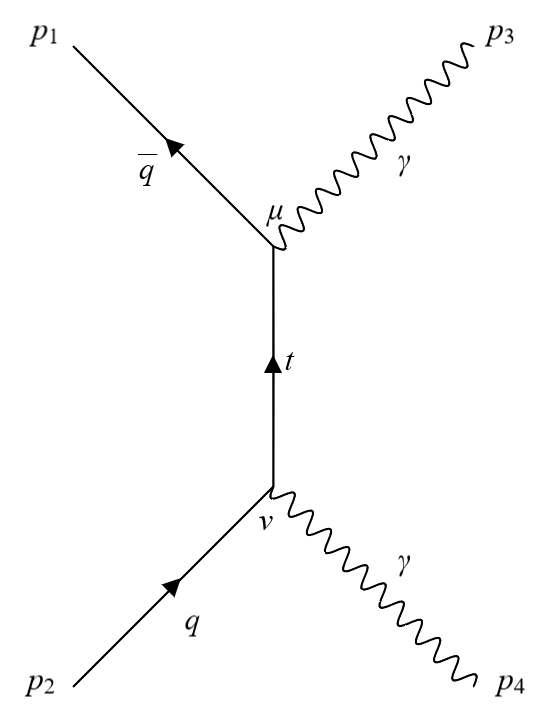
\includegraphics[width=40mm]{graphics/t.png}}
	\subfloat[u-Kanal]{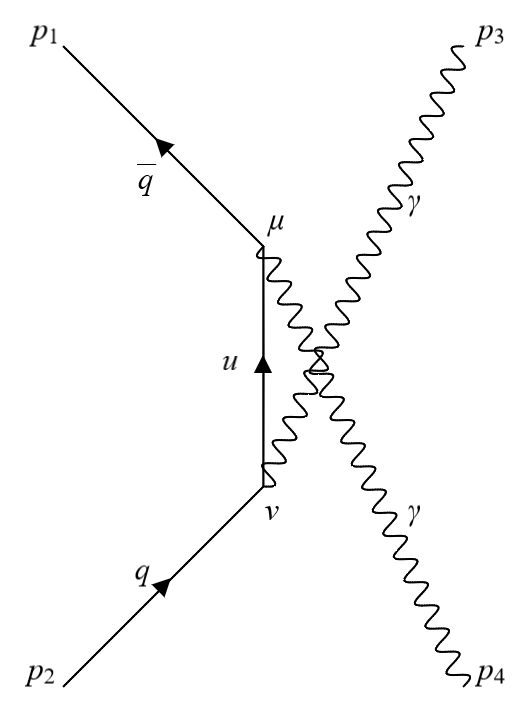
\includegraphics[width=40mm]{graphics/u.png}}
	\caption{Feynman-Diagramme des Diphoton-Prozesses führender Ordnung}
	\label{feynman-diagramme}
\end{wrapfigure}
Zunächst wird der differentielle Wirkungsquerschnitt des partonischen Diphoton-Prozesses $q\overline{q} \rightarrow \gamma \gamma$ aus den Feynman-Regeln der Quantenelektrodynamik (QED) in führender Ordnung hergeleitet. Es werden hochrelativistische Quarks betrachtet, deren Ruhemasse vernachlässigt werden kann.

In \textit{\autoref{feynman-diagramme}} sind die Feynman Diagramme führender Ordnung gezeigt. Hieraus können die Matrixelemente aus \textit{\autoref{Matrixelem_1}} abgeleitet werden. Es werden die Notation $\gamma^\mu p_\mu=\cancel{p}$, die Mandelstam-Variablen, sowie $\epsilon_\mu(p_i) \equiv \epsilon_{\mu, \lambda_i}$ verwendet, um die Matrixelemente zu vereinfachen (siehe \textit{\autoref{Matrixelem_2}}). $\lambda_i$ beschreibt die Polarisation des Photons.
\begin{equation}
\begin{aligned}
\mathcal{M}_t = \overline{\nu}\left(p_1\right) \left(-iQ_qe\gamma^\mu\right) \epsilon^*_\mu\left(p_3\right) \left(\frac{\gamma^\alpha \left(p_{1,\alpha} - p_{3, \alpha}\right)}{\left(p_1 - p_3\right)^2}\right) \left(-iQ_qe\gamma^\nu\right) \epsilon^*_\nu\left(p_4\right) u\left( p_2\right) \\
\mathcal{M}_u = \overline{\nu}\left(p_1\right) \left(-iQ_qe\gamma^\rho\right) \epsilon^*_\rho\left(p_4\right) \left(\frac{\gamma^\beta \left(p_{1,\beta} - p_{4, \beta}\right)}{\left(p_1 - p_4\right)^2}\right) \left(-iQ_qe\gamma^\sigma\right) \epsilon^*_\sigma\left(p_3\right) u\left( p_2\right)
\end{aligned}
\label{Matrixelem_1}
\end{equation}
\begin{equation}
\begin{aligned}
\mathcal{M}_t = -\frac{Q_q^2e^2}{t}\left[ \overline{\nu}(p_1) \gamma^\mu \epsilon^*_{\mu, \lambda_3} \left(\cancel{p}_1 - \cancel{p}_3\right) \gamma^\nu \epsilon^*_{\nu, \lambda_4} u(p_2)\right] \\
\mathcal{M}_u = -\frac{Q_q^2e^2}{u}\left[ \overline{\nu}(p_1) \gamma^\rho \epsilon^*_{\rho, \lambda_4} \left(\cancel{p}_1 - \cancel{p}_4\right) \gamma^\sigma \epsilon^*_{\sigma, \lambda_3} u(p_2)\right]
\end{aligned}
\label{Matrixelem_2}
\end{equation}
Die Vierervektoren sind wie in \textit{\autoref{label}} gewählt und in \textit{\autoref{label}} aufgeführt. Die Mandelstam-Variablen ergeben sich zu:
\begin{equation}
t  = -4 p^2 \cos^2\left(\frac{\theta}{2}\right) \quad \text{und} \quad u = (p_1-p_4)^2 = -4p^2 \sin^2\left(\frac{\theta}{2}\right)~.
\end{equation} 
\begin{equation}
	p_1 = \left(\begin{array}{c}p \\ 0 \\ 0 \\ p\end{array}\right) \quad 	p_2 = \left(\begin{array}{c}p \\ 0 \\ 0 \\ -p\end{array}\right) \quad p_3 = \left(\begin{array}{c}p \\ \sin(\theta)p \\ 0 \\ \cos(\theta)p \end{array}\right) \quad p_4 = \left(\begin{array}{c}p \\ -\sin(\theta)p \\ 0 \\ -\cos(\theta)p \end{array}\right)
\end{equation}
Das totale Matrixelement wird durch Summation der Anteile des u- und t-Kanals berechnet: 
\begin{equation}
\begin{aligned}
\mathcal{M} = \mathcal{M}_u + \mathcal{M}_t &= \mathcal{F} \left[\overline{\nu}(p_1) \left(\frac{\Gamma_t}{a}  +
\frac{\Gamma_u}{b} \right) u(p_2) \right] \\
&= \mathcal{F} \left[ \overline{\nu}(p_1) \Gamma u(p_2)\right]~,
\end{aligned}
\end{equation}
wobei die Ersetzungen \autoref{label} gewählt wurden.
\begin{equation}
\begin{split}
\Gamma_t = \gamma^\mu \epsilon^*_{\mu, \lambda_3} (\cancel{p}_1- \cancel{p}_3)  \gamma^\nu \epsilon^*_{\nu, \lambda_4} \quad &\text{und} \quad \Gamma_u = \gamma^\rho \epsilon^*_{\rho, \lambda_4} (\cancel{p}_1- \cancel{p}_4)  \gamma^\sigma \epsilon^*_{\sigma, \lambda_3} \\
\text{sowie} \quad \mathcal{F} = \frac{Q_q^2e^2}{4p^2} \quad &\text{und} \quad \Gamma = \frac{\Gamma_t}{\cos^2\left(\frac{\theta}{2}\right)}  +
\frac{\Gamma_u}{\sin^2\left(\frac{\theta}{2}\right)} \\
\cos^2\left(\frac{\theta}{2}\right) = a \quad &\text{und} \quad \sin^2\left(\frac{\theta}{2}\right) = b
\end{split}
\end{equation}
Bei der Berechnung des gemittelten Quadrats des Betrages des Matrixelementes, müssen die möglichen Anfangszustände der Quarks und Endzustände der Photonen berücksichtigt werden. Während die Endzustände eine Summe über mögliche Helizitäten $s_3, s_4$ und Polarisationen $\lambda_3, \lambda_4$ ergeben, können die Quarks drei verschiedene Farbzustände und jeweils zwei verschiedene Helizitäten annehmen, sodass die Anfangszustände einen Faktor $1/12$ liefern:
\begin{equation}
\left\langle  \abs{\mathcal{M}}^2\right\rangle = \frac{1}{12} \sum_{s_3, s_4} \sum_{\lambda_3, \lambda_4} \abs{\mathcal{M}}^2~.
\end{equation}
Um die Summe über die Helizitäten auszuführen, verwenden wir Casimirs Trick:
\begin{equation}
\sum_{Hel.} \abs{\mathcal{M}}^2 = \mathcal{F}^2 \sum_{Hel.}  \left[ \overline{\nu}(p_1) \Gamma u(p_2)\right] \left[\overline{\nu}(p_1) \Gamma u(p_2)\right]^* = \mathcal{F}^2~\text{Tr}\left[ \Gamma \cancel{p}_2 \overline{\Gamma} \cancel{p}_1 \right]
\end{equation}
Wobei $\overline{\Gamma} = \gamma^0\Gamma^\dagger\gamma^0 = \frac{\overline{\Gamma}_t}{a} + \frac{\overline{\Gamma}_u}{b}$ die Dirac-Adjungierte bezeichnet. Für die Dirac-adjungierten $\overline{\Gamma}_t, \overline{\Gamma}_u$ ergibt sich:
\begin{equation}
\overline{\Gamma}_t = \gamma^\nu  \epsilon_{\nu, \lambda_4} (\cancel{p}_1- \cancel{p}_3)  \gamma^\mu \epsilon_{\mu, \lambda_3} \quad \text{und} \quad \overline{\Gamma}_u = \gamma^\sigma \epsilon_{\sigma, \lambda_3} (\cancel{p}_1- \cancel{p}_4)  \gamma^\rho \epsilon_{\rho, \lambda_4} ~.
\end{equation}
\autoref{label} wird damit zu:
\begin{equation}
\text{Tr}\left[ \Gamma \cancel{p}_2 \overline{\Gamma} \cancel{p}_1 \right] = \text{Tr}\left[\frac{1}{a^2} \Gamma_t \cancel{p}_2 \overline{\Gamma}_t \cancel{p}_1 + \frac{1}{ab} \Gamma_t \cancel{p}_2 \overline{\Gamma}_u \cancel{p}_1 + \frac{1}{ba} \Gamma_u \cancel{p}_2 \overline{\Gamma}_t \cancel{p}_1 + \frac{1}{b^2} \Gamma_u \cancel{p}_2 \overline{\Gamma}_u \cancel{p}_1\right]~.
\end{equation}
Bei Einsetzen von \textit{\autoref{label}} in \textit{\autoref{label}} ergeben sich Terme in folgendem Schema:
\begin{equation}
T_{ij} = \frac{1}{12} \sum_{\lambda_3, \lambda_4} \mathcal{F}^2~\text{Tr}\left[ \frac{1}{ij} \Gamma\left(i\right) \cancel{p}_2 \overline{\Gamma}\left(j\right) \cancel{p}_1 \right] \quad \text{mit} \quad i,j \in \left\lbrace a,b\right\rbrace~.
\end{equation}
Hierbei wird $\Gamma(a) = \Gamma_t$ und $ \Gamma(b) = \Gamma_u$ identifiziert. Zunächst wird in \textit{\autoref{label}} der Fall $i = j$ evaluiert, wobei diverse Spur-Methoden und Identitäten der Dirac-Matrizen verwendet werden.
\begin{equation}
\begin{aligned}
T_{aa} &= \frac{\mathcal{F}^2}{12a^2} \sum_{\lambda_3, \lambda_4}~\text{Tr}\left[ \gamma^\mu \epsilon^*_{\mu,\lambda_3} (\cancel{p}_1- \cancel{p}_3)  \gamma^\nu \epsilon_{\nu, \lambda_4}^* \cancel{p}_2 \gamma^{\nu'} \epsilon_{\nu', \lambda_4} (\cancel{p}_1- \cancel{p}_3)  \gamma^{\mu'} \epsilon_{\mu', \lambda_3} \cancel{p}_1 \right] \\
&= \frac{\mathcal{F}^2}{12a^2} \sum_{\lambda_3, \lambda_4}\epsilon^{*\mu}_{\lambda_3}\epsilon^{\mu'} _{\lambda_3} \epsilon^{*\nu}_{\lambda_4}\epsilon^{\nu'}_{\lambda_4}~\text{Tr}\left[ \gamma_\mu (\cancel{p}_1- \cancel{p}_3)  \gamma_\nu \cancel{p}_2 \gamma_{\nu'} (\cancel{p}_1- \cancel{p}_3)  \gamma_{\mu'} \cancel{p}_1\right]\\
&\overset{\text{(2.15)}}{=}\frac{\mathcal{F}^2}{12a^2}~g^{\mu\mu'}g^{\nu\nu'}~\text{Tr}\left[ \gamma_\mu (\cancel{p}_1- \cancel{p}_3)  \gamma_\nu \cancel{p}_2 \gamma_{\nu'} (\cancel{p}_1- \cancel{p}_3)  \gamma_{\mu'} \cancel{p}_1\right] \\
&=\frac{\mathcal{F}^2}{12a^2}~\text{Tr}\left[ \gamma_\mu (\cancel{p}_1- \cancel{p}_3)  \gamma_\nu \cancel{p}_2 \gamma^{\nu} (\cancel{p}_1- \cancel{p}_3)  \gamma^{\mu} \cancel{p}_1\right]\\
&=\frac{\mathcal{F}^2}{12a^2}~\text{Tr}\left[-2\gamma^\mu(\cancel{p}_1- \cancel{p}_3) \cancel{p}_2 (\cancel{p}_1- \cancel{p}_3)\gamma^\mu \cancel{p}_1\right] \\
&=\frac{\mathcal{F}^2}{3a^2}~\text{Tr}\left[(\cancel{p}_1- \cancel{p}_3) \cancel{p}_2 (\cancel{p}_1- \cancel{p}_3)\cancel{p}_1\right] \\
&=\frac{8\mathcal{F}^2}{3a^2}(p_3\cdot p_2)(p_3\cdot p_1)
\end{aligned}
\end{equation}
Wobei die Vollständigkeitsrelation für reale Photonen \textit{\autoref{label}} verwendet wurde. Es folgt analog:
\begin{equation}
T_{bb} = \frac{8\mathcal{F}^2}{3b^2}(p_4\cdot p_2)(p_4\cdot p_1)
\end{equation}
\begin{equation}
\sum_{\lambda = 1}^{2} \epsilon^\mu_{\lambda} \epsilon^{*\nu}_{\lambda} = -g^{\mu \nu}
\label{Vollständigkeit}
\end{equation}
Für $i \neq j$ ergibt sich:
\begin{equation}
\begin{aligned}
T_{ab} &= \frac{\mathcal{F}^2}{12ab}~\text{Tr}\left[\gamma_\mu(\cancel{p}_1- \cancel{p}_4)  \gamma_\nu \cancel{p}_2 \gamma^\mu (\cancel{p}_1- \cancel{p}_3)  \gamma^\nu \cancel{p}_1 \right] \\
&=\frac{\mathcal{F}^2}{12ab}~\text{Tr}\left[ -2 \cancel{p}_2 \gamma_\nu (\cancel{p}_1- \cancel{p}_4)   (\cancel{p}_1- \cancel{p}_3)  \gamma^\nu \cancel{p}_1 \right] \\
&=  \frac{4\mathcal{F}^2}{3ab} \left[\left( p_1\cdot p_2\right) \left[ -2 \left( p_1 \cdot p_4 \right) + \left(p_3 \cdot p_4\right)\right] - (p_1\cdot p_3)(p_2\cdot p_4) + (p_2\cdot p_3)(p_1\cdot p_4)\right]
\end{aligned}
\end{equation}
und analog:
\begin{equation}
T_{ba} = \frac{4\mathcal{F}^2}{3ab} \left[\left( p_1\cdot p_2\right) \left[ -2 \left( p_1 \cdot p_3 \right) + \left(p_3 \cdot p_4\right)\right] - (p_1\cdot p_4)(p_2\cdot p_3) + (p_1\cdot p_3)(p_2\cdot p_4)\right]
\end{equation}
Beim Einsetzen der expliziten Vierervektoren aus \autoref{label}, fällt auf, dass $T_{ab} + T_{ba} = 0$. Wir haben nun die Summe über die Helizitäten ausgeführt und können damit \autoref{label} umschreiben zu:
\begin{equation}
\begin{aligned}
\left\langle  \abs{\mathcal{M}}^2\right\rangle &= \frac{8}{3}\mathcal{F}^2 \left(\frac{1}{a^2}(p_3\cdot p_2)(p_3\cdot p_1) + \frac{1}{b^2} (p_4\cdot p_2)(p_4\cdot p_1) \right) \\
&= \frac{2}{3}Q_q^4e^4\left[\frac{1-\cos^2\left(\theta\right)}{\cos^4\left(\frac{\theta}{2}\right)} + \frac{1-\cos^2\left(\theta\right)}{\sin^4\left(\frac{\theta}{2}\right)}\right] \\
&=\frac{4}{3} Q_q^4e^4\frac{1+\cos^2(\theta)}{\sin^2(\theta)} = \frac{4}{3} Q_q^4e^4\cosh(2\eta)~.
\end{aligned}
\end{equation}
Hierbei ist  $\eta = -\ln\left(\tan\left(\frac{\theta}{2}\right)\right)$ die Pseudo-Rapidität.
\section{Differentieller Wirkungsquerschnitt des partonischen Prozesses}
Mithilfe Fermis goldener Regel kann aus dem Betragsquadrat des Übergangsmatrixelementes der Wirkungsquerschnitt berechnet werden.
Im Schwerpunktsystem mit vernachlässigbaren Ruhemassen ergibt sich als Zusammenhang \textit{\autoref{zwischen}}, wobei $\text{d}\Omega = \sin(\theta)\text{d}\theta\text{d}\varphi$ das Raumwinkelelement und $s = (p_1 + p_2)^2$ das Betrag der Schwerpunktsenergie bezeichnet.
\begin{equation}
\sigma = \frac{1}{64\pi^2s} \int \left\langle  \abs{\mathcal{M}}^2\right\rangle \text{d}\Omega = \frac{1}{32\pi s} \int \left\langle  \abs{\mathcal{M}}^2\right\rangle \sin(\theta) \text{d}\theta
\end{equation}
Für den differentiellen Wirkungsquerschnitt $\derivative{\sigma}{\theta}$ ergibt sich \textit{\autoref{label}}, wobei ein Symmetriefaktor $\frac{1}{2}$ hinzukommt, da die beiden Photonen im Endzustand identisch sind.
\begin{equation}
\derivative{\sigma}{\theta} = \frac{1}{2} \cdot \frac{Q_q^4e^4}{24\pi s}\frac{1+\cos^2(\theta)}{\sin(\theta)} ~.
\end{equation}
Per Kettenregel lässt sich der differentielle Wirkungsquerschnitt in Abhängigkeit von $\eta$ bestimmen:
\begin{equation}
\derivative{\sigma}{\eta} =\derivative{\theta}{\eta}\derivative{\sigma}{\theta} =  \frac{Q_q^4e^4}{48\pi s}(1+\tanh^2(\eta))~.
\end{equation}
\section{Hadronischer Diphoton Prozess}
Aufgrund des Confinement kommen Quarks nicht als freie Teilchen vor, sodass lediglich der hadronische Prozess $pp \rightarrow \gamma \gamma$ beobachtet werden kann.  Die Protonen besitzen hierbei
\begin{wrapfigure}{r}{0.35\textwidth}
	\includegraphics[width=45mm]{graphics/Kinematik}
	\caption{Kinematik der Stoßprozesse im Labor- und Schwerpunktssystem}
\end{wrapfigure}
 zwei up-Quarks und ein down-Quark als Valenzquarks, sowie verschiedene Quark-Antiquark-Paare als Seequarks. Prallen zwei Photonen in einem Beschleuniger, beispielsweise dem $\texttt{LHC}$ zusammen, mit hohen Energien aufeinander, wird die Substruktur des Protons aufgelöst und die Konstituenten des Hadrons können miteinander interagieren. Bei diesen Interaktionen können die Quarks dann als quasi-freie Teilchen betrachtet werden.

Das Schwerpunktsystem der Quarks unterscheidet sich im Allgemeinen vom Schwerpunktsystem der Protonen, welches im Folgenden als Laborsystem bezeichnet wird. Der Impulsbruchteil eines Quarks innerhalb eines Hadrons ist nicht fest definiert, sodass ihm zunächst einen unbestimmten Bruchteil $\xi$ des Gesamtimpulses zugeordnet wird. Das Proton wird nun in einem System betrachtet, indem es eine sehr hohe Energie  $E \gg m_p$ besitzt, sodass seine Ruhemasse vernachlässigt werden und sein Vierervektor als $\textbf{p}_p = (E, 0, 0, E)$ geschrieben werden kann. Im vorliegenden System können die Transversalimpulse der Partonen vernachlässigt werden, sodass ihr Vierervektor geschrieben werden kann als:
\begin{equation}
\textbf{p}_q = (\xi E, 0, 0, \xi E) = \xi \textbf{p}_p ~.
\end{equation}
Findet bei einer Interaktion ein Impulsübertrag $\textbf{q}$ statt, so geht der Vierervektor des Partons $\xi \textbf{p}_p \rightarrow (\xi \textbf{p}_p + \textbf{q})$ über. Bei Betrachtung der invarianten Masse beider Zustände \textit{\autoref{label}} kann nach dem Impusbruchteil $\xi$ aufgelöst werden (siehe \textit{\autoref{label}}).
\begin{equation}
\left(\xi \textbf{p}_p\right)^2 = m_q^2 \quad \text{und} \quad \left(\xi \textbf{p}_p + q\right)^2 = \left(\xi \textbf{p}_p\right)^2 + 2\xi \textbf{p}_p \cdot \textbf{q} + \textbf{q}^2 = m_q^2
\end{equation}
\begin{equation}
2\xi \textbf{p}_p \cdot \textbf{q} + \textbf{q}^2 = 0 \quad \Rightarrow \quad \xi = \frac{-\textbf{q}^2}{2\textbf{p}_p\cdot \textbf{q}} = x
\end{equation}
Das $x$ in \textit{\autoref{text}} ist hierbei die Bjorken-Skalenvariable. Sie repräsentiert bei hohen Proton-Impulsen den Impulsbruchteil, den ein Parton im Proton trägt. 

Da es nicht möglich ist die Impulsbruchteile vor der Reaktion zu kennen, wird der Prozess im Schwerpunktsystem der kollidierenden Protonen beschrieben. Hier folgt der Impulsbruchteil $x$ einer Wahrscheinlichkeitsverteilung, der \textit{Partondichtefunktion} (PDF) $f_{i,h}(x, Q^2)$. Diese PDFs beschreiben die Wahrscheinlichkeitsdichte, bei einer Energieskala $Q^2 = -\textbf{q}^2$, das entsprechende Parton $i$ mit dem Impulsbruchteil $x$ im Hadron $h$ zu finden. Sie können nicht aus ersten Prinzipien abgeleitet und müssen experimentell bestimmt werden. 

Die Partondichtefunktionen können genutzt werden, um einen Ausdruck für den totalen Wirkungsquerschnitt $pp \rightarrow \gamma \gamma $ zu finden. Ist der totale Wirkungsquerschnitt eines partonischen Prozesses zwischen den Partonen $i$ und $j$, bei den festgelegten Impulsbruchteilen $x_1$ und $x_2$ und der Energieskala $Q^2$ (genannt $\tilde{\sigma}_{i,j}(x_1, x_2, Q^2)$) bekannt, dann kann mithilfe der PDF der totale Wirkungsquerschnitt $\sigma_{i,j}$ für die Reaktion der Partonen $i$ und $j$ bei dem Zusammenstoß von zwei Protonen berechnet werden. In \textit{\autoref{text}} ist die Kennzeichnung des Hadrons vernachlässigt.  
\begin{equation}
\sigma_{i,j} = \int f_i(x_1, Q^2)f_j(x_2, Q^2) \tilde{\sigma}_{i,j}(x_1, x_2, Q^2)\text{d}x_1\text{d}x_2
\end{equation}
Der totale Wirkungsquerschnitt ergibt sich dann als Summe aller möglichen $\sigma_{i,j}$, wobei im Diphoton-Prozess lediglich $i=q=\overline{j}$ beitragen:  
\begin{equation}
\sigma = \sum_{q} \left(\sigma_{q,\overline{q}} + \sigma_{\overline{q},q} \right)~. 
\end{equation}
In Abschnitt \textit{\autoref{text}} wurde bereits der differentielle Wirkungsquerschnitt für den partonischen Prozess $\sigma_p$ im Schwerpunktsystem der Konstituenten berechnet. $\tilde{\sigma}_{q,\overline{q}}(x_1, x_2, Q^2)$ kann nach \textit{\autoref{label}} berechnet werden.
\begin{equation}
\tilde{\sigma}_{q,\overline{q}}(x_1, x_2, Q^2) = \int \frac{\text{d}\sigma_{p}}{\text{d}\eta}\left(x_1,x_2, Q^2\right)\text{d} \eta
\end{equation}
\textit{\autoref{label}} gilt im Schwerpunktsystem der Partonen und muss im Folgenden in das Laborsystem transformiert werden. Weiterhin muss die Mandelstam-Variable $s$, die das Quadrat der Schwerpunktsenergie der Partonen darstellt, in Abhängigkeit von $x_1, x_2$ ausgedrückt werden. Für die Partonen $q$ und $\overline{q}$ mit den Impulsbruchteilen $x_1$ und $x_2$ lassen sich im Schwerpunktsystem der beiden Hadronen ihre Vierervektoren schreiben als \textit{\autoref{label}}, wobei $E$ die Strahlenergie bezeichnet.
\begin{equation}
\textbf{p}_q = \left(x_1E, 0, 0, x_1E\right) \quad \text{und} \quad \textbf{p}_{\overline{q}} = \left(x_2E, 0, 0, -x_2E\right)
\end{equation}
Mit \textit{\autoref{label}} ergibt sich die Schwerpunktenergie zu:
\begin{equation}
\sqrt{s} = 2\sqrt{x_1x_2}E~.
\end{equation}
Im folgenden werden Variablen im Laborsystem ungestrichen und Variablen im Schwerpunktsystem der Partonen gestrichen benannt. DIe Pseudo-Rapidität, die sich additiv bei Inertialsystemwechsel verhält, transformiert sich, wenn sich das Schwerpunktsystem der Partonen mit der Geschwindigkeit $\beta$ zum Laborsystem bewegt, nach \textit{\autoref{label}}.
\begin{equation}
\eta' = \eta + \frac{1}{2}\ln(\frac{1-\beta}{1+\beta}) \quad \Rightarrow \quad \frac{\text{d}\eta'}{\text{d}\eta} = 1 
\end{equation}
Damit ergibt sich für den Wirkungsquerschnitt im Laborsystem: 
\begin{equation}
\frac{\text{d}\sigma_p}{\text{d}\eta} = \frac{\text{d}\eta'}{\text{d}\eta} \frac{\text{d}\sigma_p}{\text{d}\eta'} = \frac{Q_q^4e^4}{48\pi s}(1+\tanh^2(\eta')).
\end{equation}
Die Geschwindigkeit $\beta$ ergibt sich mit den Dreierimpulsen $\vec{p}$ zu \textit{\autoref{text}}.
\begin{equation}
\beta = \frac{\abs{\vec{p}_q + \vec{p}_{\overline{q}}}}{m_q + m_{\overline{q}}} = \frac{(x_1 - x_2)E}{(x_1 + x_2)E} = \frac{x_1 - x_2}{x_1 + x_2}
\end{equation}
Durch Einsetzen der gefunden Ausdrücke für $s, \eta'$, und $\beta$ in \textit{\autoref{text}}, ergibt sich mit $Q^2 = 2 x_1 x_2 E^2$ insgesamt für die differentiellen Wirkungsquerschnitt im Laborsystem:
\begin{equation}
\derivative{\sigma_p}{\eta}\left(x_1, x_2, Q^2, q\right) = \frac{Q_q^4e^4}{96\pi Q^2} \left(1+\tanh^2\left(\eta + \frac{1}{2}\ln(\frac{x_2}{x_1})\right)\right)~.
\end{equation}
Schließlich können mithilfe von \textit{\autoref{label}}, \textit{\autoref{label}} und \textit{\autoref{label}} die Ausdrücke \textit{\autoref{label}} für den totalen und \textit{\autoref{label}} für den dreifach differentiellen Wirkungsquerschnitt gefunden werden.
\begin{equation}
\sigma = \sum_{q} \int \left[f_q(x_1, Q^2)f_{\overline{q}}(x_2, Q^2) +f_{\overline{q}}(x_1, Q^2)f_{q}(x_2, Q^2) \right] \derivative{\sigma_p}{\eta} \text{d}x_1\text{d}x_2\text{d}\eta
\end{equation}
\begin{equation}
\frac{\text{d}^3\sigma}{\text{d}x_1\text{d}x_2\text{d}\eta} = \sum_{q} \left[f_q(x_1, Q^2)f_{\overline{q}}(x_2, Q^2) +f_{\overline{q}}(x_1, Q^2)f_{q}(x_2, Q^2) \right] \derivative{\sigma_p}{\eta} 
\end{equation}
\section{Reweightning zwischen PDF-Sets}
Das quantitative Ergebnis von \textit{\autoref{???}} hängt von dem verwendeten Fit an die Partondichtefunktionen ab. Je nach Messung und Anpassung ergeben sich dabei kleine Unterschiede zwischen den verschiedenen Sets. Das \textit{Reweight} entspricht einem Umrechnungsfaktor zwischen differentiellen Wirkungsquerschnitten, die mit verschiedenen Fits von Partondichtefunktionen berechnet wurden. Aus \textit{\autoref{???}} kann, bis auf die Quarkladung,  $\derivative{\sigma_p}{\eta}$ aus der Summe herausgezogen werden, sodass sich für die Gewichte zwischen den PDF-Sets $f^{(1)}$ und $f^{(2)}$ \textit{\autoref{text}} ergibt.
\begin{equation}
w\left(x_1, x_2\right) = \frac{ \sum_{q} Q_q^4 \left[f_q^{(1)}(x_1, Q^2)f_{\overline{q}}^{(1)}(x_2, Q^2) +f_{\overline{q}}^{(1)}(x_1, Q^2)f_{q}^{(1)}(x_2, Q^2) \right]}{\sum_{q} Q_q^4 \left[f_q^{(2)}(x_1, Q^2)f_{\overline{q}}^{(2)}(x_2, Q^2) +f_{\overline{q}}^{(2)}(x_1, Q^2)f_{q}^{(2)}(x_2, Q^2) \right]}
\end{equation}
\chapter{Maschinelles Lernen und tiefe neuronale Netzwerke}
\section{Einführung in Maschinelles Lernen}
\textbf{Motivation:}
Die Berechnung eines differentiellen Wirkungsquerschnitts eines Prozesses aus den zugrundeliegenden Feynman-Diagrammen, kann schnell sehr kompliziert werden. Oft sind diese Aufgaben analytisch nicht oder nur noch sehr aufwändig lösbar, sodass numerische Methoden bemüht werden müssen. Diese fortgeschrittenen Methoden können in der Praxis sehr rechenintensiv sein und viele Ressourcen beanspruchen. Algorithmen, die maschinelles Lernen verwenden, können je nach Typ und Komplexität jedoch sehr effizient und im Vergleich mit herkömmlichen numerischen Methoden signifikant schneller sein. Ein ML-Algorithmus ist zwar nicht in der Lage, den differentiellen Wirkungsquerschnitt analytisch aus den zugrundeliegenden Feynman-Diagrammen in erster Instanz zu berechnen, er kann die Funktion jedoch durch die Vorarbeit eines rechenaufwändigeren Algorithmus erlernen. Der Vorteil liegt hierbei darin, die aufwändigen numerischen Methoden zur Berechnung einer ausreichenden Anzahl von Phasenraumpunkten nur einmalig durchzuführen, mit diesen das DNN zu trainieren, um anschließend eine größere Anzahl an Punkten zu generieren.

Im Folgenden werden die Möglichkeiten eines solchen Einsatzes von ML-Algortihmen untersucht und evaluiert.

\textbf{Einführung:} Das Konzept \glqq Maschinelles Lernen\grqq~befasst sich damit, aus Informationen, beispielsweise Messwerte, ein statistisches Modell zu entwickeln, das die Muster hinter den Lerndaten erkennt und übertragen kann. Wir unterscheiden dabei die Teilgebiete:
\begin{itemize}
	\setlength\itemsep{0.1cm}
	\setlength{\parskip}{0.1cm}
	\item Klassifizierung und 
	\item Regression
\end{itemize}
\textbf{Klassifizierung} ordnet Objekten ihre jeweilige Gruppe, auch genannt \glqq Label\grqq~zu. Dies geschieht auf Grundlage der Eigenschaften eines Objektes, den sogenannten \glqq Features\grqq~.
Wir werden uns im Folgenden mit \textbf{Regression} beschäftigen, wobei hier anstatt einer diskreten Zuordnung eine reelle Zahl ausgegeben wird. Betrachten wir eine Funktion $f: \mathbb{R}^n \rightarrow \mathbb{R}, \mathbf{x} \mapsto f(\mathbf{x})$, bezeichnen wir die Einträge des Vektors $\mathbf{x}$ als Features und den Funktionswert $f(\mathbf{x}) \in \mathbb{R}$ als Label. Am Beispiel des hadronischen Diphoton Prozess \textit{\autoref{label}}, kann man $x_1, x_2, \eta$ als Features und den zugehörigen differentiellen Wirkungsquerschnitt als Label identifizieren. 
Im \textbf{überwachten} Lernen sind alle Trainingsdaten mit Labels versehen, sodass die Vorhersage des Modells mit dem wahrend Ergebnis abgeglichen werden und das Netz seine Parameter entsprechend anpassen kann, um minimale Abweichung zu erreichen. 

Die konkrete Art des Machine-Learning, die in dieser Arbeit untersucht wird, ist das Deep-Learning, dessen Prinzip auf künstlichen neuronalen Netzwerken beruht. Diese neuronalen Netze sollen im folgenden verwendet werden, um einen Regressionsalgorithmus zu entwickeln, der gegebenenfalls hochdimensionale Funktionen erlernen und damit die Effizienz der numerischen Berechnung von differentiellen Wirkungsquerschnitten steigern kann. 
\section{Neuronale Netze}
Eine Veranschaulichung des Konzeptes eines neuronalen Netzes ist in \textit{\autoref{label}} gezeigt.
Den Grundbaustein eines DNN, in dem die elementaren Berechnungen durchgeführt werden, stellt das Neuron dar, dessen Name durch das biologische Nervensystem inspiriert ist.
Diese Neuronen, die auch Units oder Nodes genannt werden, können unterschiedlich stark aktiviert sein. Die Nodes sind in Schichten, genannt Layern, organisiert, zwischen denen die Ausgabewerte der Neuronen hin- und hertransferiert werden. Die Units des Layers $l$ nehmen als Funktionsargumente die Aktivierung von Neuronen der Schicht $l-1$ und geben ihrerseits wieder einen reellen Wert aus. Während im ersten Layer, genannt Input-Layer, die Aktivierung der Neuronen durch den Wert der eingehenden Features gegeben ist, beherbergt die letzte Schicht, der sogenannte Output-Layer nur noch eine Node, dessen Aktivierung die Vorhersage des Netzes darstellt. \\
\begin{wrapfigure}{r}{0.5\textwidth}
	\includegraphics[width=65mm]{graphics/NeuralNetwork}
	\caption{Konzeptzeichnung eines mehrschichtigen Perzeptron, kann noch verändert werden}
\end{wrapfigure}
Es wird sich im folgenden auf vollständig verbundene Feedforward-Netze beschränkt. Während sich hierbei vollständig verbunden darauf bezieht, dass ein Neuron mit allen Neuronen der vorhergehenden Schicht verbunden ist, versteht man unter Feedforward-Netzen, dass die Ausgabe von Units der Schicht $l-1$ nur Neuronen in Layer $l$ beeinflusst. \\
\\\
Jedes Neuron stellt zunächst eine lineare Funktion von den Ausgaben des vorhergegangen Layers $l-1$ dar, die im Vektor $\mathbf{y}_{l-1}$ zusammengefasst sind. Wir stellen die Ausgabe des $n$-ten Neurons der Schicht l, bezeichnet mit $y_l^n$, als Skalarprodukt zwischen den Gewichten der Node $\mathbf{w}_{l}^n$ dar, wobei zusätzlich das Bias $b_l^n$ addiert wird. Auf diese Lineare Funktion wird anschließend eine nichtlineare Aktivierungsfunktion $\sigma$ angewendet, die es dem Netz ermöglicht nichtlineare Zusammenhänge zu erlernen.
\begin{equation}
y_l^n = \sigma\left(\mathbf{w}_{l}^n \cdot \mathbf{y}_{l-1} + b_{l}^n\right)
\end{equation}
Für den ersten Layer gilt  $\mathbf{y}_0 = \mathbf{x}$, die Features entsprechen also $y_0$. In unserem vollständig verbundenen Netz erhalten wir also pro Node eine lineare Gleichung der Form \textit{\autoref{text}}. Insgesamt können wir die Rechenoperation, die in einem Layer stattfindet also als Matrixmultiplikation formulieren. Die Vektoren $\mathbf{w}_{l}^n$ werden hierbei zu den Zeilen der Matrix $\mathbf{W}_l$, die  $b_{l}^n$ fassen wir in Vektoren zusammen.
\begin{equation}
\mathbf{y}_l = \sigma\left(\mathbf{W}_l\cdot \mathbf{y}_{l-1} + \mathbf{b}_l\right)
\end{equation}
Im Neuron des Output-Layers findet schließlich die Ausgabe des Funktionswertes $y$ statt. Das Ziel ist es nun, die Abweichung des Ausgabewertes $y$ des Netzes vom wahren Wert $\tilde{y}$ zu minimieren. Mathematisch wird die Abweichung als eine Metrik definiert und das Erlernen der freien Parameter eines künstlichen neuronalen Netzes wird damit zum Optimierungsproblem. Im Kontext von ML wird die zu minimierende Metrik, die abhängig von allen Gewichten $\mathbf{W}$ und Biases $\mathbf{b}$ ist, als Kostenfunktion (Cost-Function) oder Verlustfunktion (Loss-Function) bezeichnet, wobei hier eine mögliche Wahl die mittlere quadratische Abweichung ist.
\begin{equation}
C\left(\mathbf{W}, \mathbf{b}\right) = \frac{1}{N}\sum_{i=1}^{N}\left(y^{(i)} - \tilde{y}^{(i)}\right)^2
\end{equation}
Als Kostenfunktion kann prinzipiell jede Metrik verwendet werden, die zielführend erscheint und es muss je nach Problemstellung abgewogen werden, welche Wahl die besten Ergebnisse liefert.
Da die analytische Berechnung von Extremstellen der Verlustfunktion von neuronalen Netzen nicht möglich ist, greifen wir auf \textit{Gradient-Descent} zurück. Hierbei wird, beim Output-Layer beginnend, der Gradient der Kostenfunktion berechnet und per Kettenregel zum vorherigen Layer fortgepflanzt. Diesen Vorgang, so für alle Nodes einen Gradienten zu berechnen, nennt sich Backpropagation und führt in der Anwendung auf die Methode des automatischen Ableitens zurück. Die Gradienten werden immer gemittelt für eine Anzahl an Trainingspunkten, genannt Batch, an Trainingspunkten berechnet und auf die Gewichte angewendet, sodass man sich einem lokalen, oder auch globalen, Minimum nähern kann (Stochastic Gradient Descent, SGD).
\section{Training und Hyperparameter}
Man nennt Parameter, die der Programmierende im Vornherein festlegen muss und die nicht vom Algorithmus erlernt werden, Hyperparameter. Wir sprechen im Weiteren über folgende Hyperparameter, wobei wir nicht zwischen solchen Hyperparametern, die die Architektur des Netzes bestimmen und Trainingsparametern, die das Lernverhalten bestimmen, differenzieren:
\begin{multicols}{2}
	\begin{itemize}
		\setlength\itemsep{0.1cm}
		\setlength{\parskip}{0.1cm}
		\item Anzahl der Layer und Nodes
		\item Kostenfunktion
		\item Aktivierungsfunktion der Neuronen
		\item Initialisierung der Gewichte
		\item Optimizer(Lernart) 
		\item Learning-Rate(Lernrate)
		\item Batch-Größe
		\item Anzahl der Trainingsepochen
		\item Normalisierung
	\end{itemize}
\end{multicols}
Die Architektur eines neuronalen Netzes wird durch die Anzahl an \textbf{Layer und Nodes} festgelegt.
Tiefere neuronale Netze mit größeren Anzahlen an Neuronen sind in der Lage kompliziertere Sachverhalte genauer zu lernen, allerdings steigt die Anzahl an zu trainierenden Parametern und auszuführenden Rechnungen. Bei zu komplexen Modellen für simple Sachverhalte mit wenigen Trainingspunkten kommt es häufig zur Überanpassung, bei der sich das Modell zu sehr auf die vorliegenden Daten spezialisiert und seine Generalisierungsfähigkeit verliert.

Die \textbf{Loss-Funktion} bestimmt das Lernverhalten des Netzes maßgeblich, denn sie ist es die letztendlich optimiert wird, um die Gradienten zu erhalten. 

Die \textbf{Aktivierungsfunktion} bricht die Linearität des Netzes und sorgt dafür, dass dieses nichtlineare Funktionen erlernen kann.  Die Form und Ableitung der Aktivierungsfunktion bestimmt den Gradienten während der Backpropagation. Gegebenenfalls kann sie auch dazu genutzt werden, die Ausgabe eines Neurons zu regulieren. Speziell für Aktivierungsfunktionen mit verschwindenden Ableitungen, besonders die namensgebende Aktvierung \textit{ReLU}, kann das \textit{Dying-ReLU-Problem} auftreten. Hierbei wurden durch große Gradienten die Gewichte eines Neurons so verändert, dass es, fast unabhängig von seinen Funktionswerten, nur noch Null ausgibt\footnote{Null speziell für ReLU}. Da die Ableitung in diesem Definitionsbereich ebenfalls Null ist, kann sich das Neuron nicht regenerieren und trägt im Folgenden nicht mehr zum Lernprozess des Netzes bei.

An welchem Punkt des hochdimensionalen Phasenraums der Kostenfunktion der Lernprozess beginnt, wird von der \textbf{Initialisierung} festgelegt. Die Initialisierung der Gewichte ist eng verknüpft mit der verwendeten Aktivierungsfunktion, sodass sich bereits spezielle Initialisierungsmethoden für bestimmte Aktivierungen etabliert haben, wie zum Beispiel HeNormal für ReLU-Aktivierung. %TODO refs für HeNormal und ReLU

Die hier besprochenen Lernalgorithmen basieren auf Gradientenabstieg. Für die konkrete Implementation des Gradient-descent, die sich gegebenenfalls an die vorliegende Situation anpasst, wird \textbf{Optimizer} genannt. Die \textbf{Learning-Rate} ist hierbei der Faktor, mit dem der Gradient skaliert wird, bevor er auf die Gewichte angewendet wird. Diese muss hierbei so gewählt werden, dass das Lernen weder in einem zu hohen lokalen Maximum zum Erliegen kommt, noch zu groß ist um den Tiefpunkt des Minimums zu erreichen. 

Die \textbf{Batch-Größe} beschreibt, wie viele Objekte in einem Durchgang vom neuronalen Netz behandelt werden. Große Batch-Größen dämpfen Ausreißer und beschleunigen die Trainingszeit, wobei ein Training mit kleineren Batches detailreicher und genauer sein kann. 

Die Anzahl \textbf{Trainingsepochen} beschreibt, wie oft während des Lernvorgangs über die Trainingsdaten iteriert wird. Die Präzision eines neuronalen Netzes konvergiert idealerweise, daher kann eine Abbruchbedingung als minimale Verbesserung zwischen Epochen festgelegt werden. 

Hat man Features, deren numerische Reichweite stark auseinandergeht, kann es sich lohnen die Eingabewert zu \textbf{normalisieren}. Das bedeutet, alle Features auf ein festgelegtes Intervall, zum Beispiel $I=[1,0]$ anzupassen. So wird verhindert, dass einem Feature mit großem numerischen Wert zu viel Bedeutung zugeordnet wird.

Das Finden der besten Hyperparameter ist ein weiteres Optimierungsproblem, das abgesehen von der Suche der besten Gewichte gelöst werden muss. Für die Methoden des Grid- oder Random-Search wird ein Gitter an Hyperparametern erstetllt. Anschließend werden im ersten Fall alle und im zweiten lediglich zufällige Gitterpunkte trainiert und evaluiert. Fortgeschrittenere Methoden der Hyperparameteroptimierung wie Bayesian-Search oder Hyperband, sollen in kürzerer Zeit bessere Parameter finden. Die Hyperparameteroptimierung kann sehr aufwändig sein. 

\textbf{Implementierung mit Keras und Tensorflow}
Die Implementierung des ML-Algorithmus wird in dieser Arbeit mit der Open-Source Python-Bibliothek \texttt{TensorFlow} und \texttt{Keras} stattfinden. Keras fungiert hierbei als eine high-level API für TensorFlow. Das Erstellen eines Netzes wird mit den Modulen vereinfacht und sowohl Loss-Funktion, Optimizer als auch Initialisierungen sind bereits implementiert. Es können sowohl vorgefertigte Layer angepasst werden, als auch Layer und Trainingsroutine selbst schreiben, wobei die vorgefertigten Layer über einige Methoden verfügen, die den Umgang mit dem Netz komfortabler machen und das Speichern und Laden vereinfachen. 

\section{Transfer-Learning}
Um die hohen Zeit- und Rechenkosten des Trainings zu verringern, können bereits trainierte Modelle an ein neues Problem anpasst werden. Außerdem kann mit dem sogenannten \textbf{Transfer-Learning}, die Menge an Daten, die benötigt wird, um ein brauchbares Modell zu erhalten, signifikant verringert werden. \\
Die Grundidee des Transfer-Learning besteht darin, dass der Algorithmus sein bereits erlerntes statistisches Modell auf eine andere Situation überträgt und gegebenenfalls nur noch die numerischen Ausgaben anpassen muss. Es ist beobachtet worden, dass Transfer-Learning die folgenden Vorteile bringt: % TODO ist das in dieser Referenz auch beobachtet worden?
\begin{itemize}
	\setlength\itemsep{0.1cm}
	\setlength{\parskip}{0.1cm}
	\item Höherer Start, höhere Asymptote und höhere Steigung der Lernkurve
	\item signifikant weniger Messwerte benötigt, um brauchbare Ergebnisse zu erreichen
\end{itemize}
Wir machen Nutzen von beiden Aspekten, da wir einerseits die Trainingszeit reduzieren und sich andererseits die Zeit zur Datengeneration verkürzt. Konkret wird im Laufe dieser Arbeit das Transfer-Learning verwendet, um die differentiellen Wirkungsquerschnitt berechnet mit einem PDF-Set, auf selbige, berechnet mit einem anderen PDF-Set, zu übertragen. Dabei wird von beiden angesprochenen Aspekten profitiert, da einerseits die Trainingszeit reduziert werden kann, als auch die Zeit zur Datengeneration verkürzt wird.

Im Folgenden wird kurz auf den Ablauf von Transfer-Learning für künstliche neuronale Netze eingegangen:
\begin{itemize}
	\setlength\itemsep{0.1cm}
	\setlength{\parskip}{0.1cm}
	\item Zunächst wird ein sogenanntes Source-Model an einer Source-Datenmenge bis zur Konvergenz trainiert. 
	\item Eine kleinere Datenmenge an Zielwerten wird erstellt.
	\item Die oberste oder einige der oberen Schichten (sprich der Output-Layer und wenige darunterliegende Layer) werden entfernt.
	\item Die Gewichte der restlichen Layer werden zunächst fixiert, um diese nicht durch große Gradienten zu zerstören.
	\item Die entfernten Schichten werden mit neuen, trainierbaren Neuronen ersetzt
	\item Schließlich wird das neue Modell an der kleinern Datenmenge trainiert.
	\item Als optionaler Letzter Schitt wird das sogenannte \textit{Fine-Tuning}(FT) eingesetzt. Bei diesem werden die fixierten Gewichte wieder gelöst.
\end{itemize}


\section{Monte-Carlo-Integration}
Monte-Carlo-Integration unterscheidet sich von anderen numerischen Integrationsmethoden vor allem dadurch, dass die Konvergenz der Integration keine Abhängigkeit von der Dimensionalität des Integrals aufweist. Monte-Carlo-Methoden konvergieren hierbei immer mit $\propto \frac{1}{\sqrt{N}} $, wobei $N$ die Anzahl der ausgewerteten Phasenraumpunkte ist. Es wird hierbei Gebrauch vom Gesetz der Großen Zahlen gemacht und die Integrale mittels Wahrscheinlichkeitstheorie gelöst. \\
\\\
Betrachte eine Funktion $f: \Omega \subseteq \mathbb{R}^n \rightarrow \mathbb{R}, \mathbf{x} \mapsto f(\mathbf{x})$ und definiere ihren Erwartungswert $\left\langle f(\mathbf{X})\right\rangle $ auf $\Omega$, wobei $\mathbf{X}$ uniform auf $\Omega$ gezogen wird.
\begin{equation}
\left\langle f(\mathbf{X})\right\rangle  = \left\langle f\right\rangle  = \frac{1}{\norm{\Omega}}\int_{\Omega} f(\mathbf{x}) \text{d}\mathbf{x} 
\end{equation}
Es wird nun das Gesetz der Großen Zahlen angewendet und somit einen Schätzer für den Erwartungswert von $f$ (\textit{\autoref{text}}) gefunden.
\begin{equation}
\tilde{\left\langle f \right\rangle } = \frac{1}{N} \sum_{i=1}^{N} f(\mathbf{x}_i) \quad \text{mit} \quad \lim_{N\rightarrow \infty} \frac{1}{N} \sum_{i=1}^{N} f(\mathbf{x}_i) = \left\langle f \right\rangle
\end{equation}
Da de Erwartungswert nicht exakt berechnet werden kann, weil es nicht möglich ist $f$ an unendlich vielen Punkten zu evaluieren, wird verwendet, dass der Schätzer gegen den Erwartungswert konvergiert und genähert $\tilde{\left\langle f \right\rangle } \approx \left\langle f \right\rangle$. Die Geschwindigkeit der Konvergenz der Näherung kann erhöht werden, indem in \textit{\autoref{ref}} eine produktive Eins in Form einer Wahrscheinlichkeitsdichte $\rho: \Omega \subseteq \mathbb{R}^n \to \mathbb{R}_{\geq 0}, x \mapsto \rho(x)$ mit $\int_{\Omega} \rho(x) \text{d}x = 1$ eingeführt wird (\textit{\autoref{text}})
\begin{equation}
I = \int_{\Omega} f(\mathbf{x}) \text{d}x =  \int_{\Omega} \frac{f(\mathbf{x})}{\rho(\mathbf{x})}\rho(\mathbf{x}) \text{d}\mathbf{x} = \left\langle \left(\frac{f}{\rho}\right) \right\rangle_{\rho} 
\end{equation}
Dabei stellt $\left\langle \left(\frac{f}{\rho}\right) \right\rangle_{\rho}$  den Erwartungswert von $\frac{f}{q}$ unter der Bedingung dar, dass die $\mathbf{x}_i$ nach der Wahrscheinlichkeitsverteilung $\rho(\mathbf{x})$ gezogen werden. Der Schätzer ergibt sich dann zu \textit{\autoref{text}}.
\begin{equation}
I \approx \tilde{\left\langle \left(\frac{f}{\rho}\right) \right\rangle}_{\rho}  = \frac{1}{N}\sum_{i=1}^{N}\frac{f(\mathbf{x}_i)}{\rho(\mathbf{x}_i)}
\end{equation}
%TODO Notation für Schätzer, Erwartungswert etc klären
Die Konvergenz der MC-Integration ist am Schnellsten, wenn sich die Varianz von \textit{\autoref{text}} minimiert. Die Varianz ist gegeben durch \textit{\autoref{text}}
\begin{equation}
\text{Var}\left(\frac{f}{\rho}\right) = \left\langle\left(\frac{f}{\rho} - \left\langle \frac{f}{\rho}\right\rangle \right)^2 \right\rangle = \left\langle \left(\frac{f}{\rho}\right)^2 \right\rangle - \left\langle\frac{f}{\rho} \right\rangle^2 \approx \frac{1}{N} \sum_{i=1}^{N}\left(\frac{f(\mathbf{x}_i)}{\rho(\mathbf{x}_i)}\right)^2 - I^2
\end{equation}
Die Varianz minimiert sich also, wenn jeder Summand aus \textit{\autoref{text}} gleich groß ist. Der Vorgang die Wahrscheinlichkeitsdichte $\rho$ an die Form unserer zu integrierenden Funktion $f$ anzupassen, nennt man \textbf{Importance Sampling}. Hierbei zieht man absichtlich die $\mathbf{x}_i$ mit höheren Wahrscheinlichkeiten aus den Regionen, in denen auch $f$ den größten Beitrag liefert. Die Unsicherheit auf die Integration ergibt sich aus der Standardabweichung des Mittelwerts sprich:
\begin{equation}
\sigma_{\left\langle \frac{f}{\rho}\right\rangle} = \frac{1}{\sqrt{N-1}} \cdot \sqrt{\text{Var}\left(\frac{f}{\rho}\right)}
\end{equation}
Wir werden im Folgenden simple Monte-Carlo-Methoden und das Importance Sampling verwenden, um aus unseren differentiellen Wirkungsquerschnitten die totalen Wirkungsquerschnitte zu erhalten.   


\chapter{Anwendung von Maschinellem auf den Diphoton Prozess}
\section{Diphoton-Prozess auf Parton-Ebene}
% TODO wir verwenden überall den gleichen Initializer HE-Normal etc
Zunächst werden neuronale Netze zur Regression der eindimensionalen differentiellen Wirkungsquerschnitte aus \textit{\autoref{}} benutzt. Dabei werden geeignete Wertebereiche gewählt, sprich $\theta \in [\epsilon, \pi - \epsilon]$ bzw. $\eta \in [-3, 3]$, wobei wir das Verhalten des DNN für verschiedene $\epsilon$ evaluieren werden. Kleine $\epsilon$ sind hierbei interessant, weil der Wirkungsquerschnitt für $\epsilon = 0$ am Rand des Intervalls divergiert und somit das Verhalten von neuronalen Netzen an Polstellen untersucht werden kann. Die quantitativen Werte im nächsten Abschnitt sind für einen $d\overline{d} \rightarrow \gamma \gamma$-Prozess mit einer Schwerpunktsenergie von $\sqrt{s} = 200 \text{GeV}$ berechnet. Wir generieren die Trainingspunkte zufällig nach einer, wenn nicht explizit anders angegebenen, uniformen Verteilung.  
Es werden im Weiteren nur Netze mit der gleichen Anzahl an Neuronen in jedem Layer verwendet.

\textbf{Modell für $\mathbf{\frac{d\sigma}{d\eta}}$:} 
Der differentielle Wirkungsquerschnitt in Abhängigkeit der Pseudo-Rapidität ist eine gutartige Funktion ohne Pol- oder Sprungstellen. \textit{\autoref{text}} reduziert sich von der Form auf einen $\tanh^2$, dessen Wertebereich sich über $[0,1)$ erstreckt und damit schon von vornherein auf einen geeigneten Wertebereich normiert ist. Wir behandeln den Vorfaktor mit einer Skalierung der Funktionswerte, auf die wir später noch weiter eingehen werden. 
Für diese einfache Aufgabe werden die Hyperparameter wie in \textit{\autoref{label}} gewählt und keine weiteren Optimierungen, wie für die folgenden Modelle, durchgeführt. Wir werden in Zukunft standardmäßig den Kernel-Initializer HeNormal verwenden und das Bias zu Null initialisieren.
\begin{table}[hbt]
	\centering
	\begin{tabular}{|l|l|}
		\hline
		Hyperparameter & Wert \\
		\hline
		Anzahl Layer & 2 \\
		Anzahl Units & 64 \\
		Loss-Funktion & Mean-Absolute-Error \\
		Optimizer & Adam \\
		Aktivierungsfunktion & ReLU \\
		Kernel-Initializer & HeNormal \\
		Bias-Initializer & Zeros \\
		Learning-rate & 0.005 \\
		Batch-Größe & 128 \\
		Max. Epochen & 300 \\
		Anzahl Trainingspunkte & 10000\\
		\hline
	\end{tabular}
	\caption{Hyperparameter des Modells $\frac{d\sigma}{d\eta}$}
\end{table}
Das Training an sich wird von den folgenden, in Keras implementierbaren, Callbacks geregelt:
\begin{itemize}
	\item \texttt{LearningRateScheduler}: Ein Ablaufplan wird festgelegt, der für jede Epoche die zu verwendende Learning-Rate bestimmt. 
	\item \texttt{ReduceLROnPlateau}: Erzielt das Training bezogen auf eine bestimmte Metrik nicht einen Mindestfortschritt, wird die Learning-Rate reduziert.
	\item \texttt{EarlyStopping}: Erzielt das Training bezogen auf eine bestimmte Metrik für eine gewisse Zeit keinen Mindestfortschritt, wird das Training gestoppt.
\end{itemize}
Die Wahl der genauen Konfiguration der Callbacks ist in \textit{\autoref{text}} festgehalten.
Die gelernte Funktion im Vergleich mit den analytischen Werten ist in \textit{\autoref{}} gezeigt. Die Werte überlagern sich gut, sodass man auf den ersten Blick keinen Unterschied feststellen kann. Betrachtet man das Verhältnis, erkennt man, dass sich der Unterschied auf ca. $0.1\%$ beläuft. 
\begin{figure}[hbt]
	\centering
	\subfloat[Vergleich DNN - analytische Werte für \\ $\derivative{\sigma}{\eta}$]{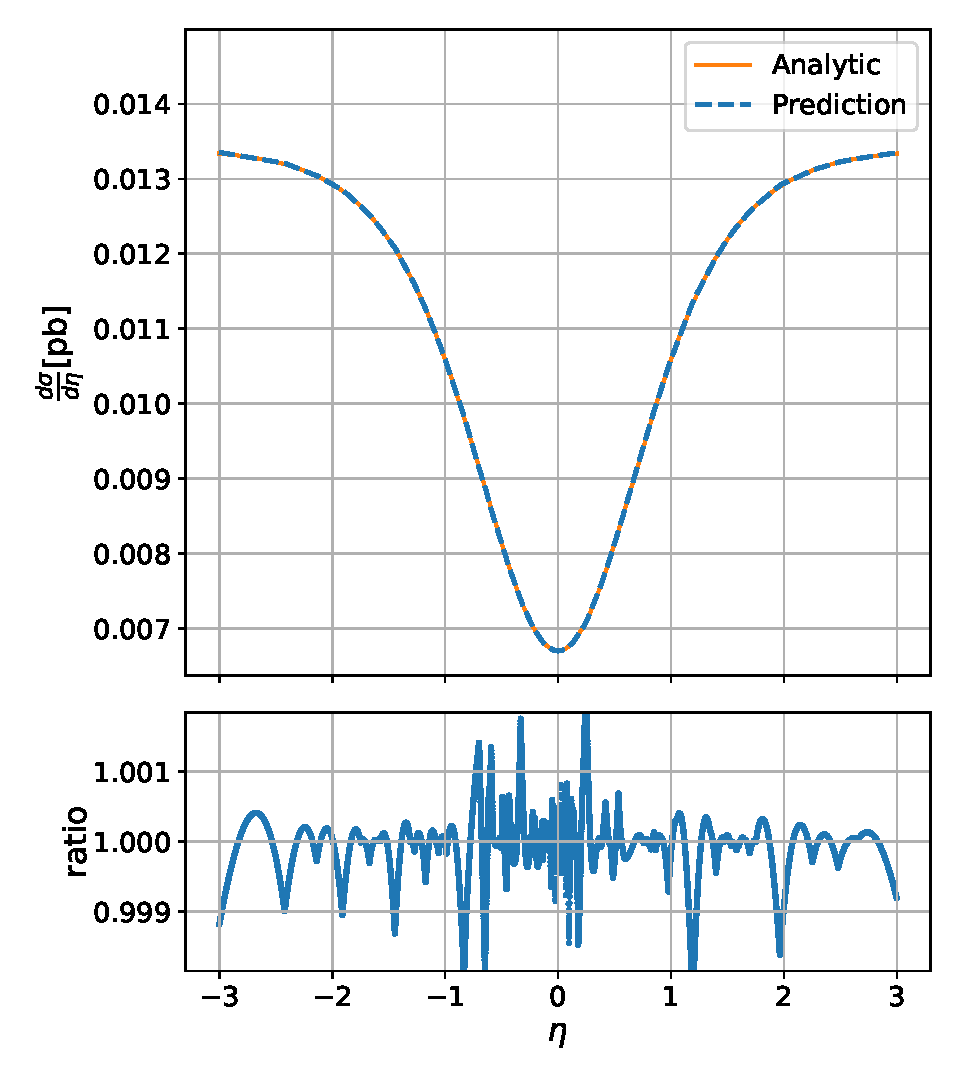
\includegraphics[width=6.5cm]{graphics/1}}
	\subfloat[Vergleich DNN - analytische Werte für $\derivative{\sigma}{\theta}$ \\  auf $\theta \in {[\epsilon, \pi - \epsilon]}$ für $\epsilon=0.163$]{	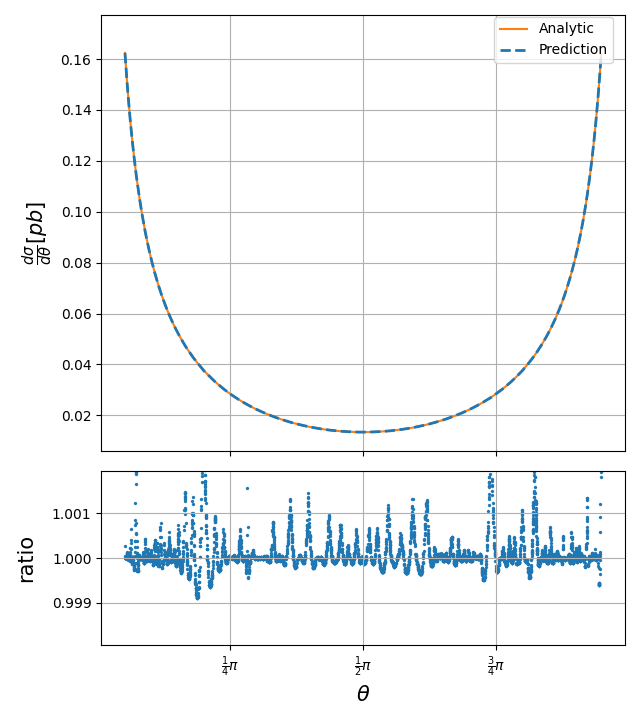
\includegraphics[width=6.5cm]{graphics/2}}
	\caption{Predictions der neuronalen Netze für den Wirkungsquerschnitt des Diphoton-Prozess auf partonischer Ebene}
	\label{partonic_eta_model}
\end{figure}

\textbf{Modell für $\mathbf{\frac{d\sigma}{d\theta}}$:} %TODO Atlas Referenz
Der Wirkungsquerschnitt in Abhängigkeit von $\theta$ unterscheidet sich vom vorherigen Modell durch seine Polstellen. Da wir numerisch nicht mit Polstellen umgehen können, müssen wir den Trainingsbereich auf $[\epsilon, \pi-\epsilon]$ einschränken. Aus physikalischer Sicht ist das legitim, da die Polstellen im Strahlengang des Speicherrings liegen und damit nicht messbar sind. Viele Detektoren, wie ATLAS, können Photonen mit Pseudo-Rapiditäten bis zu $\abs{\eta} \leq 2.5$ messen, was einem $\epsilon \approx 0.163$ entspricht. Durch Normierung der Labels auf das Intervall $[-1, 1]$, kann dem Modell der Umgang mit den Polstellen erleichtert werden. Da gute Modelle hier nicht mehr trivial gefunden werden können, wird auf eine automatische, zufällige Suche zurückgegriffen (Random-Search). Die Such-Parameter mit Ergebnis sind in \textit{\autoref{text}} festgehalten.

Es fällt auf, dass die Architektur des Modells um ein vielfaches komplizierter ist, als die des Modells für $\derivative{\sigma}{\eta}$. Einerseits ist dies aufgrund der Polstellen zu erwarten und andererseits darin begründet, dass komplexere Modelle Probleme generell präziser lösen können und daher aus der Suche hervorgehen. Die Performance des Modells ist in \textit{}\autoref{label} gezeigt. Die Präzision ist trotz der komplizierteren Funktion mit \textit{\autoref{text}} vergleichbar. Durch den Random-Search konnte ein passendes Modell gefunden werden. %TODO Netz mit gleichen Hyperparametern wie eta

Es werden zwei weitere Modelle mit den gleichen Hyperparametern auf einem Intervall $[\epsilon', \pi-\epsilon']$ mit $\epsilon' < \epsilon$ trainiert, wobei die Trainingsdaten des einen Modells nach der Verteilung \textit{\autoref{label}}(\textit{Importance Sampling(IS)}) generiert sind, um die Leistung der drei Modelle zu vergleichen. 
\begin{wrapfigure}{r}{0.5\textwidth}
	\centering
	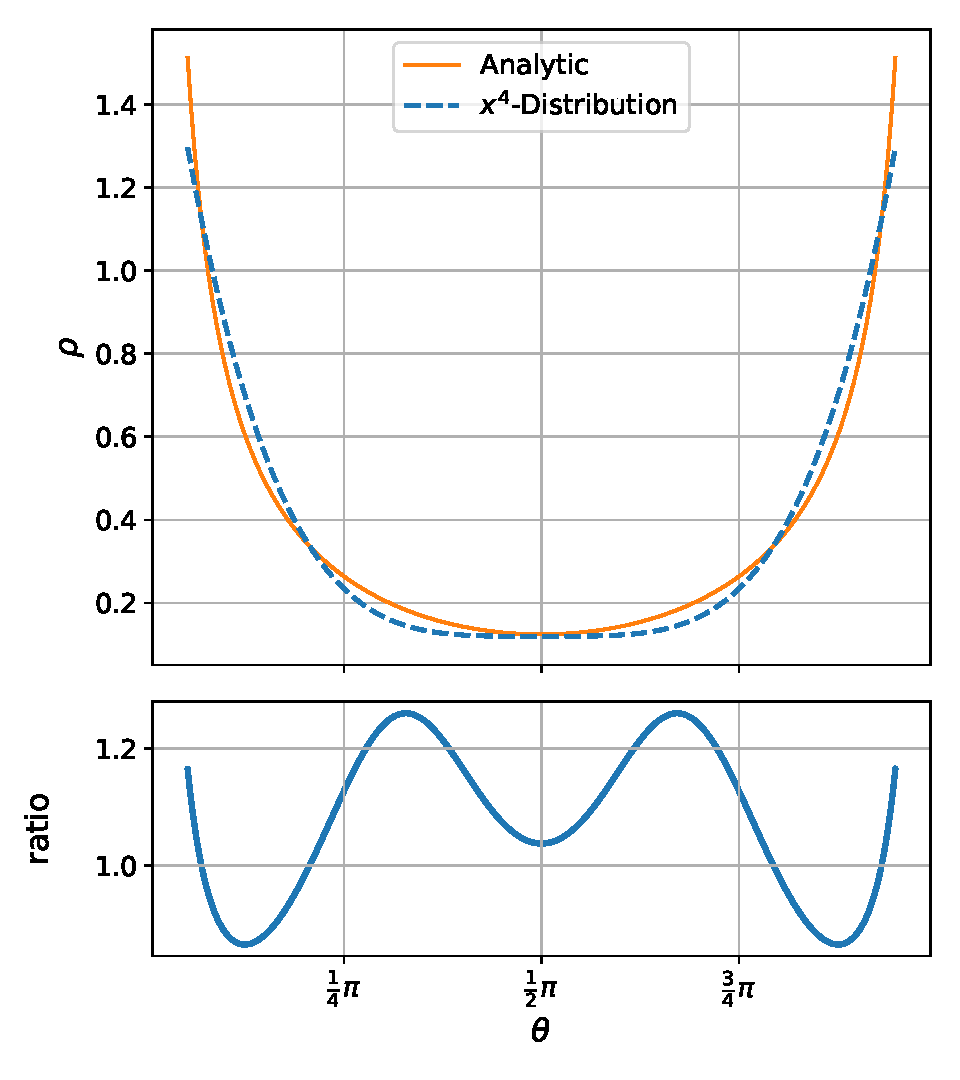
\includegraphics[width=6cm]{graphics/4}
	\caption{simples Importance Sampling, das die analytische Funktion annähern soll hier verweis auf Funktion in anhang}
\end{wrapfigure}

Die Vergleiche sind in \textit{\autoref{text}} und in \textit{\autoref{text}} für $\epsilon' = 0.01$ gezeigt. Wie zu erwarten weicht das Modell, das auf dem Intervall $[\epsilon, \pi-\epsilon]$ trainiert wurde, außerhalb seines Trainingsintervalls stark von der analytischen Funktion ab. Es trifft die Steigung der analytische Funktion am Startpunkt der Extrapolation, höhere Ableitungen vernachlässigt das Modell jedoch. Aufgrund ihres größeren Trainingsintervalls, zeigen die beiden anderen Modelle akzeptable Leistung auch nahe an den Polstellen. In \textit{\autoref{text}} kann man an einigen Stellen am Verhältnis sehen, dass das mit importance gesampelten Trainingsdaten trainierte Netz an den Polstellen besser und im Zentrum schlechter angepasst ist. In \textit{\autoref{text}} a) ist der Definitionsbereich näher an die Polstelle gelegt, um den Verbesserung des IS-gesampelten Modells besser aufzulösen. Anhand von \textit{\autoref{text}} b) wird deutlich, dass der Effekt noch größer ist, wenn keine Überfülle an Trainingsdaten vorhanden ist. Ist also der Umfang an verfügbaren Trainingsdaten klein oder wenig Rechenleistung vorhanden, kann auf Importance Sampling zurückgegriffen werden, um Modelle mit Fokus auf wichtige Bereiche zu trainieren. Dabei ist zu beachten, dass hier ein Kompromiss zwischen Verlässlichkeit nahe der Polstelle und Verlässlichkeit im Zentrum des Definitionsbereiches eingegangen wird.

In \textit{\autoref{text}} sind noch einmal der MAPE (Mean-Absolute-Percentage-Error) der verschiedenen Modelle für verschiendene Testdatensets gezeigt. Hier wird erneut deutlich, dass das Importance Sampling vor allem nützlich ist, wenn Bereiche mit hohen Funktionswerten besonders wichtig sind. Bei der Berechnung des totalen Wirkungsquerschnittes aus dem differentiellen Wirkungsquerschnitt ist genau dies der Fall.
\enlargethispage{3.cm}
\begin{figure}[H]
	\centering
	\subfloat[Vergleich DNN-analytische Werte für $\derivative{\sigma}{\theta}$ auf $\theta \in {[\epsilon’, \pi - \epsilon’]}$ für $\epsilon’=0.01$]{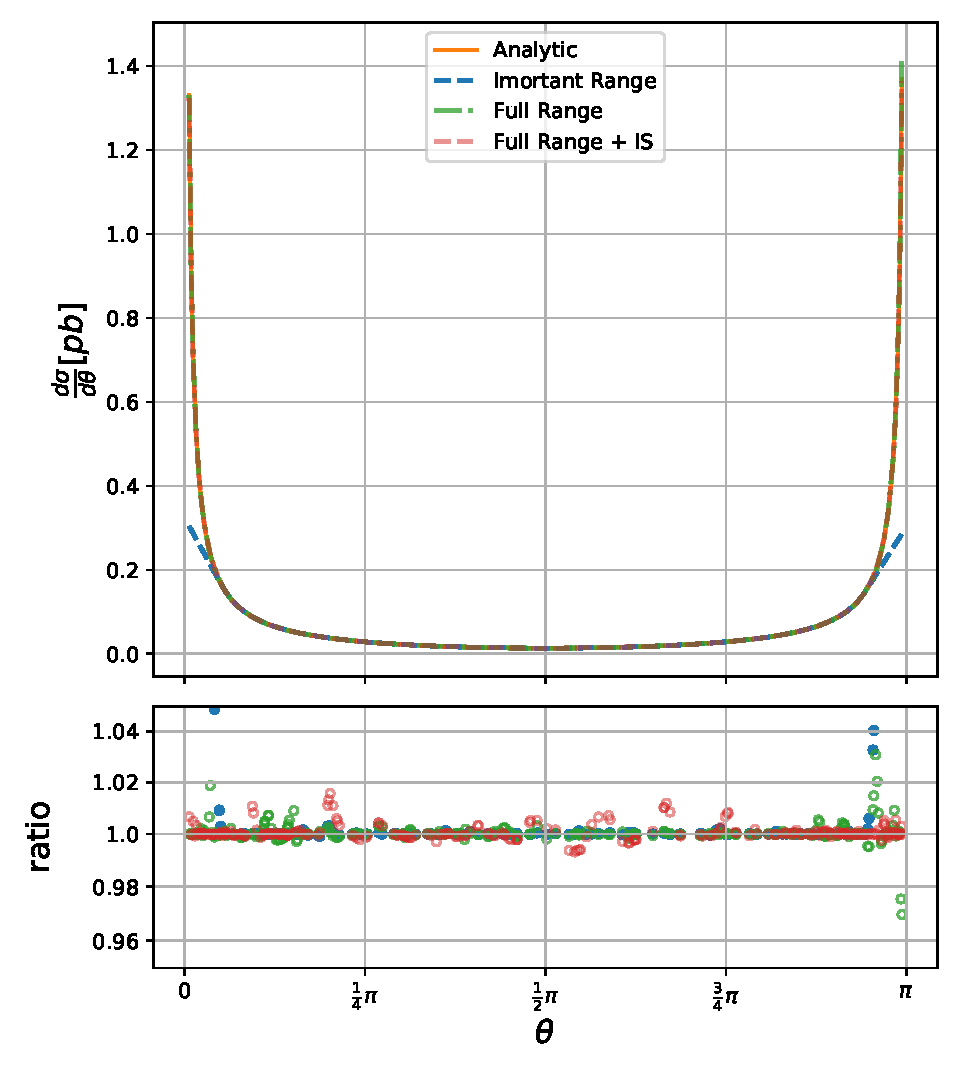
\includegraphics[width=6.5cm]{graphics/3}}
	\subfloat[MAPE für verschiedene Test-Datensets]{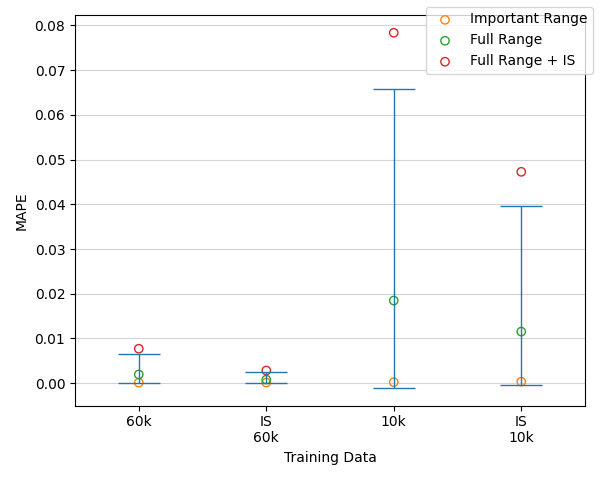
\includegraphics[width=6.5cm]{graphics/26}} \\
	\subfloat[Modelle mit 60000 Traningspunkten]{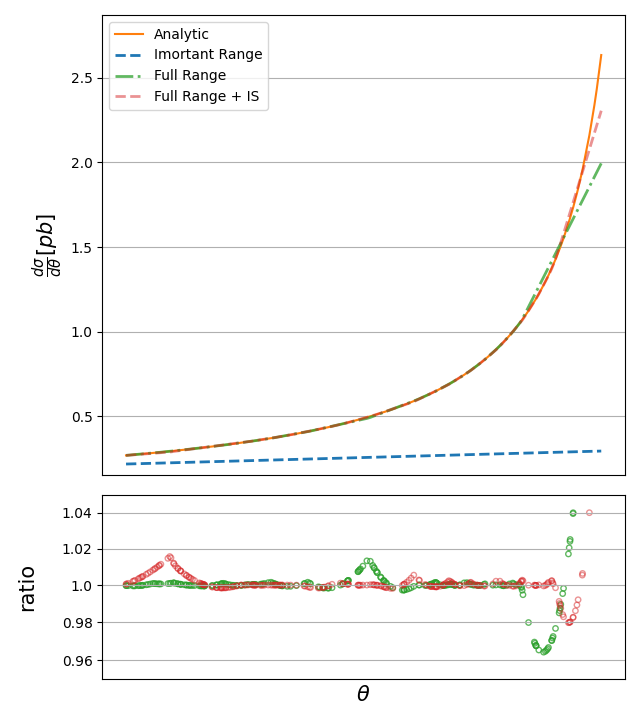
\includegraphics[width=6.5cm]{graphics/3.1}}
	\subfloat[Modelle mit 10000 Trainingspunkten]{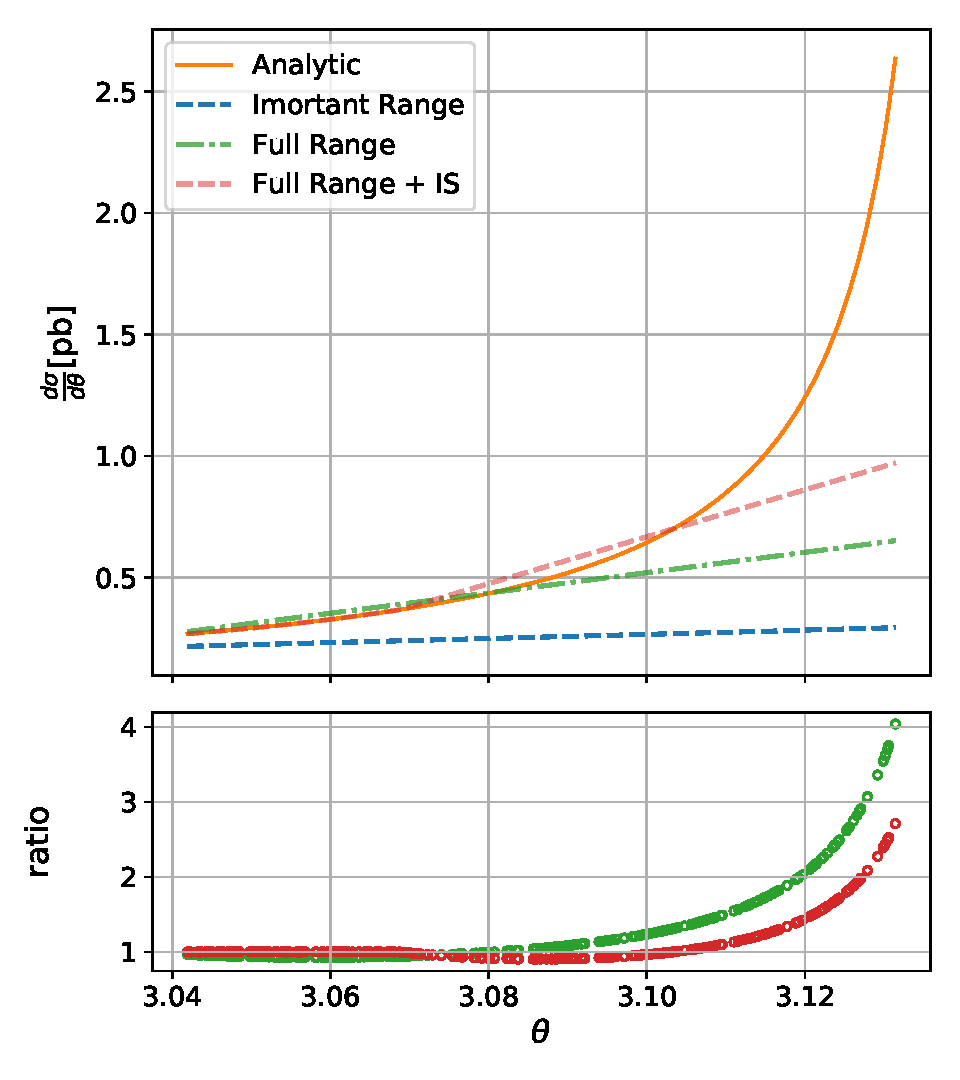
\includegraphics[width=6.5cm]{graphics/3.2}}
	\caption{Vergleich der Performance auf unterschiedlichen Intervallen von verschiedenen Theta-Modellen, die mit verschiedenen Datenmengen trainiert wurden.}
\end{figure}
\section{Diphoton-Prozess auf Hadron-Ebene}
\subsection{Allgemeines und Phasenraumschnitte}
Im Gegensatz zu den bisher diskutierten Prozessen, ist die Reaktion $pp \rightarrow \gamma \gamma$ beobachtbar und messbar. Der Wirkungsquerschnitt soll am Beispiel einer Messung im ATLAS-Detektor behandelt werden. Es werden einige Beschränkungen auf die Events angewendet, die sich an einer realen Messung orientieren und durch die Detektorgeometrie motiviert sind, da dieser nicht den gesamten Raumwinkelbereich abdecken kann. Die generierten Phasenraumpunkte werden selektiert und der Algorithmus nur an solchen Messpunkten trainiert, die auch praktisch detektierbar wären. Die verwendeten Selektionen sind angelehnt an \textit{\autoref{Siegert}} und aufgelistet in \textit{\autoref{label}}.
\begin{table}[bp]
	\centering
	\begin{tabular}{|c|c|}
		\hline
		Bereich & Cut \\
		\hline
		Photon-Energie & $\abs{p_T} > 40$ GeV \\
		Photon Winkel & $\abs{\eta_{\gamma, \gamma'}} < 2.37$ ohne $1.37 < \abs{\eta_{\gamma, \gamma'}} < 1.52$ \\
		Impulsbruchteil & $x_{1,2} < 0.7 $\\
		\hline
	\end{tabular}
	\caption{Event-Selektion für den hadronischen Diphoton-Prozess in Anlehnung an Messung von ATLAS[Ref]} %TODO ref
\end{table}
Dabei sind $\gamma$ und ${\gamma'}$ die Bezeichnungen für die beiden Photonen und $p_{T,\gamma} = p_{T,\gamma'} = p_T$ beschreibt den Impuls der produzierten Photonen transversal zum Strahlengang. \textit{\autoref{label}} ist, aufgrund der Abhängigkeit der PDF, für große $x_1, x_2$ extrem klein und fällt zusätzlich stark ab, es werden daher außerdem Ereignisse mit $x > 0.7$ herausgenommen. Dieser Schnitt vernachlässigt den Phasenraumbereich mit extrem kleinen Labels und erleichtert dem DNN den Lernprozess. 

%TODO graph der deine eta Rechnung erklärt?
Da sich das Laborsystem vom Schwerpunktsystem der kollidierenden Quarks unterscheidet, müssen wir sicherstellen, dass beide Photonen die $\eta$-Selektion erfüllen. Werden $\eta_{\gamma}$ und $\eta_{\gamma'}$ in entgegengesetzte Richtungen gemessen, berechnen sich diese aus $\eta'$ der Photonen im Schwerpunktsystem der Quarks nach: 
\begin{equation}
\eta_{\gamma} = \eta' -\frac{1}{2}\ln(\frac{x_2}{x_1}) \quad \text{sowie} \quad \eta_{\gamma'} = \eta’ + \frac{1}{2}\ln(\frac{x_2}{x_1})~.
\end{equation}
$\eta_{\gamma'}$ kann somit in Abhängigkeit von $\eta_{\gamma}$ dargestellt werden als:
\begin{equation} 
\eta_{\gamma'} = \eta_{\gamma} + \frac{1}{2}  \ln(\frac{x_2^2}{x_1^2})
\end{equation}
Für die Berechnung von \textit{\autoref{label}} verwenden wir das PDF-Set CT14nnlo von LHAPDF, wobei wir positive Beiträge von Charm- und Strange-Quark berücksichtigen und Top- und Bottom-Quark vernachlässigen. Die Strahlenergie beträgt $E = 6500 \text{GeV}$.
\subsection{Vorbereitung und Training}
Im Vergleich zu den vorhergegangenen Prozessen hat sich nun die Dimensionalität des Problems, sowie die Gutartigkeit der Funktion verändert. Die Partondichtefunktionen, die den dreidimensionalen Wirkungsquerschnitt bestimmen, fallen exponentiell mit ihren Impulsbruchteilen $x_1$ und $x_2$ ab und besitzen Polstellen für $x \rightarrow 0$\footnote{wobei die PDFs numerisch ab $x_{\text{min}} \approx 10^{-9}$ eingefroren werden.}. Die Labels variieren daher von $10^{3}~\text{pb}$ bis zu $10^{-20}~\text{pb}$. Wie sich herausgestellt hat, lässt sich diese Form und exponentielle Sensitivität für Veränderungen in $x$ mit der linearen Natur der Operationen eines DNN nur begrenzt reproduzieren. Hinzu kommt, dass eine gängige Loss-Funktion wie der Mean-Squared- oder Mean-Absolute-Error lediglich Punkte mit hohen Wirkungsquerschnitten berücksichtigen und damit die Vorhersagen schon ab einem kleinen $x$ unbrauchbar werden würden. Es wurde Lösung in der oft für ähnliche Probleme verwendeten Loss-Funktion \textit{Mean-Squared-Logarithmic-Error}(MSLE) gesucht (siehe \textit{\autoref{text}}), da es hier ausschließlich auf das Verhältnis zwischen Label und Vorhersage ankommt und damit gesichert ist, dass keine Phasenraumbereiche vernachlässigt werden. Um nicht mit negativen Werten zu arbeiten, wird generell $y \rightarrow y + 1$ transformiert. Da jedoch der Großteil der quantitativen Werte des Wirkungsquerschnittes in standardmäßig verwendeten Einheiten, sprich $1/\text{GeV}^2$ und $\text{pb}$, viel kleiner als eins ist und damit $\ln(1+y) \approx y$ gilt würde so nur ein ineffizienterer MSE implementiert werden. 
\begin{equation}
C\left(\mathbf{M}, \mathbf{b}\right) = \frac{1}{N} \sum_{i=1}^{N} \left(\ln(y^{(i)}) - \ln(\tilde{y}^{(i)})\right)^2 = \frac{1}{N} \sum_{i=1}^{N} \left(\ln(\frac{y^{(i)})}{\tilde{y}^{(i)}})\right)^2
\end{equation}
An dieser Stelle wurde ursprünglich das erste mal die Skalierung implementiert, die bereits in den diskutierten Modellen verwendet wurde. Wie sich im Laufe der Arbeit mit den künstlichen neuronalen Netzen gezeigt hat, beugt die Skalierung außerdem das Dying-ReLU-Problem (siehe \textit{\autoref{label}}) vor. Es ist aufgefallen, dass quantitativ kleine Labels dazu führen können, dass durch starke Überschätzung der Labels direkt nach der Initialisierung des Netzes, viele Neuronen bereits nach den ersten Batches absterben. Es ist entscheidend, dies zu verhindern, um brauchbare Ergebnisse zu erhalten. Während den Untersuchungen wurde beobachtet, dass es sehr mühsam ist, eine gute Initialisierung zu finden, die das Problem verhindert. Schließlich wurde auf die Skalierung der Funktionswerte zurückgegriffen.

Andere Versuche um mit dem Dying-ReLU-Problem umzugehen sind die Verwendung von Aktivierungsfunktionen mit nicht-verschwindender Ableitung wie Leaky-ReLU oder ELU (siehe \textit{\autoref{label}}), die den Nodes ermöglichen soll, sich zu regenerieren, oder die Übergabe eines \textit{Clipvalue/Clipnorm}-Parameters an den Optimizer, der den Gradienten reguliert.
 
Im Folgenden wird die Skalierung mit einem Transformator-Objekt realisiert, der die vorliegenden Labels nach $\tilde{y} \rightarrow \tilde{y}/{\tilde{y}_{min}}$
anpasst, wobei $\tilde{y}_{min}$ das kleinste Label im Trainigsdatensatz ist. Der Transformator wird mit seinen Variablen abgespeichert und kann bei Bedarf wieder initialisiert werden, um die Ausgaben des DNN auf reale Werte zurückzuskalieren. 
Da bereits ein Transformator verwendet wird, kann der Logarithmus bereits vor der Loss-Funktion angewendet werden, was einerseits flexibler in der Verwendung der Loss-Funktionen und andererseits rechnerisch effizienter ist\footnote{als den Logarithmus einzeln für jeden Batch zu berechnen´}. Die Label-Normalisierung aus dem vohergehenden Modell wurde praktisch auch im Transformator umgesetzt.

Zur Hyperparameteroptimierung verwenden wir wieder einen Random Search. Mit anderen Suchmethoden wie Bayesian Search oder Hyperband konnte keine Verbesserung der Hyperparametersuche festgestellt werden. Die Hyperparameter einer erfolgreichen Suche sind in \textit{\autoref{text}} aufgelistet. Hierbei muss man beachten, dass die Trainingspunkte zufällig generiert sind nach den Verteilungen:
\begin{equation}
\begin{aligned}
\rho(x) &= \frac{1}{(x + \alpha)\ln(\frac{x_{max} + \alpha}{x_{min}+ \alpha})} \qquad \text{mit} \qquad \alpha = 0.005 \\
\rho(\eta) &= \begin{cases}
\frac{1}{\sqrt{2\pi \sigma^2}} \exp(-\frac{(\eta - \eta_{max})^2}{2\sigma^2}) \quad & \text{für} \qquad 0 \leq \eta \leq \eta_{max}\\
\frac{1}{\sqrt{2\pi \sigma^2}} \exp(-\frac{(\eta + \eta_{max})^2}{2\sigma^2}) \quad & \text{für} \quad -\eta_{max} \leq \eta < 0
\end{cases} \quad \text{mit} \quad \sigma = 1.5
\end{aligned}
\end{equation}
Bei gegebenen Parametern und Nach Anwendung der Cuts(\textit{\autoref{label}}) beläuft sich die Sample-Effizienz auf bei gegebenen Parametern auf $\approx 40\%$. Wir trainieren also mit weniger Daten, als es auf den ersten Blick wirkt. \\
%TODO Umrechnung in pb für Grafik 8
\begin{figure}[tbp]
	\centering
	\subfloat[Schnitt in $\eta$, $ x_1 \approx x_2$]{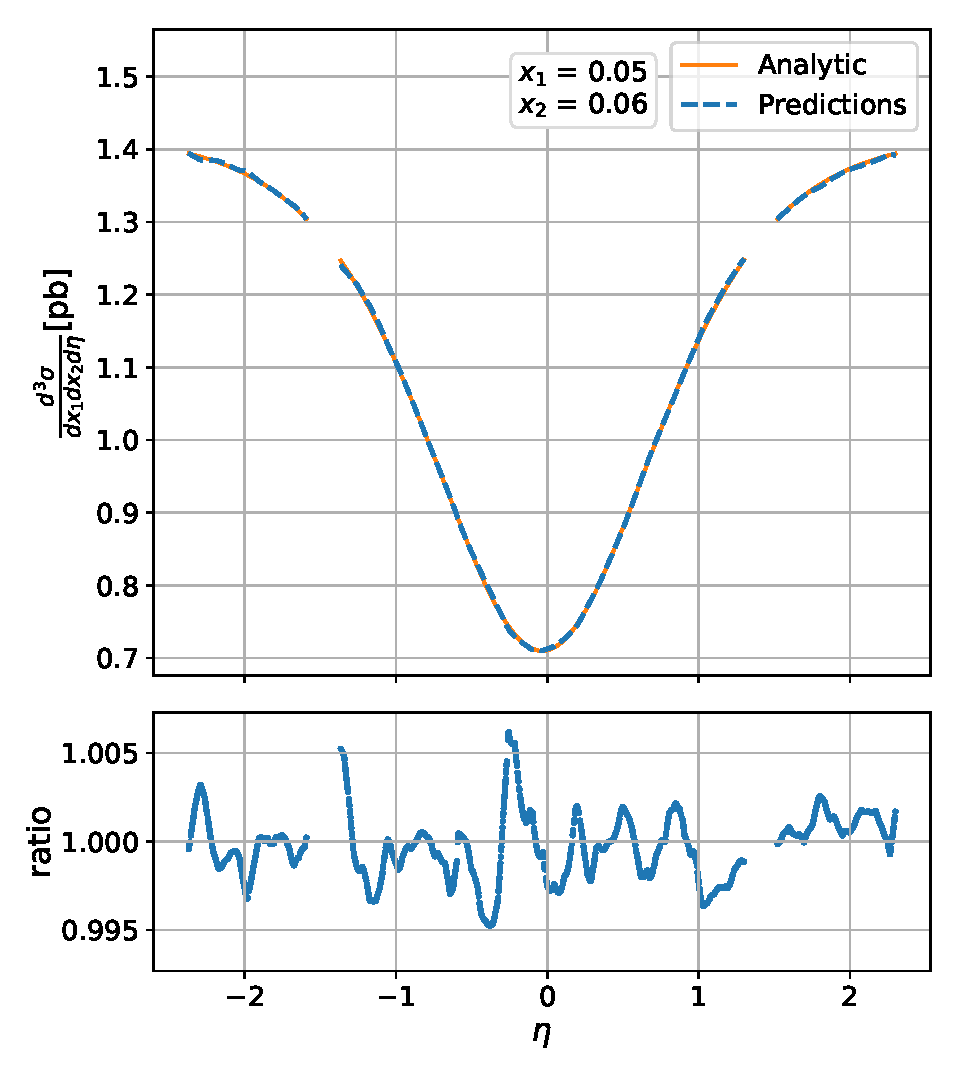
\includegraphics[width=6cm]{graphics/5}}
	\subfloat[Schnitt in $\eta$, $ x_1 \neq x_2$]{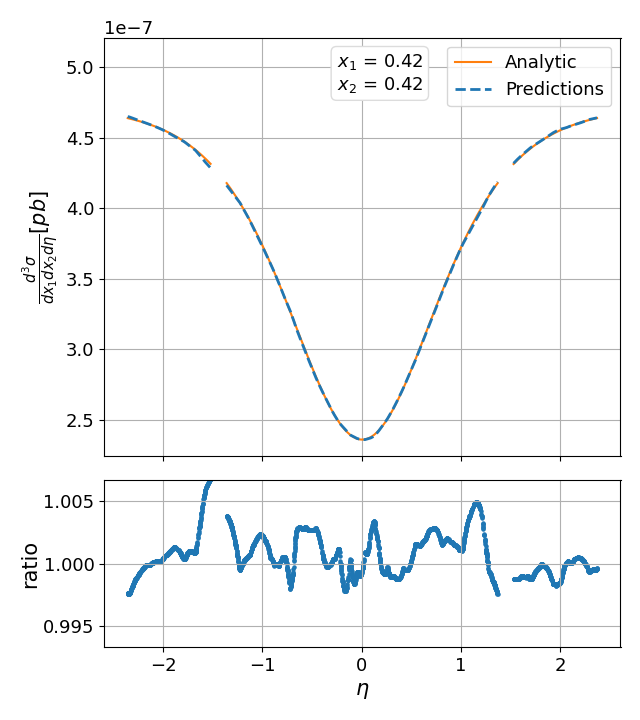
\includegraphics[width=6cm]{graphics/8}} \\
	\subfloat[Schnitt in $x_1$, $x_2$ klein]{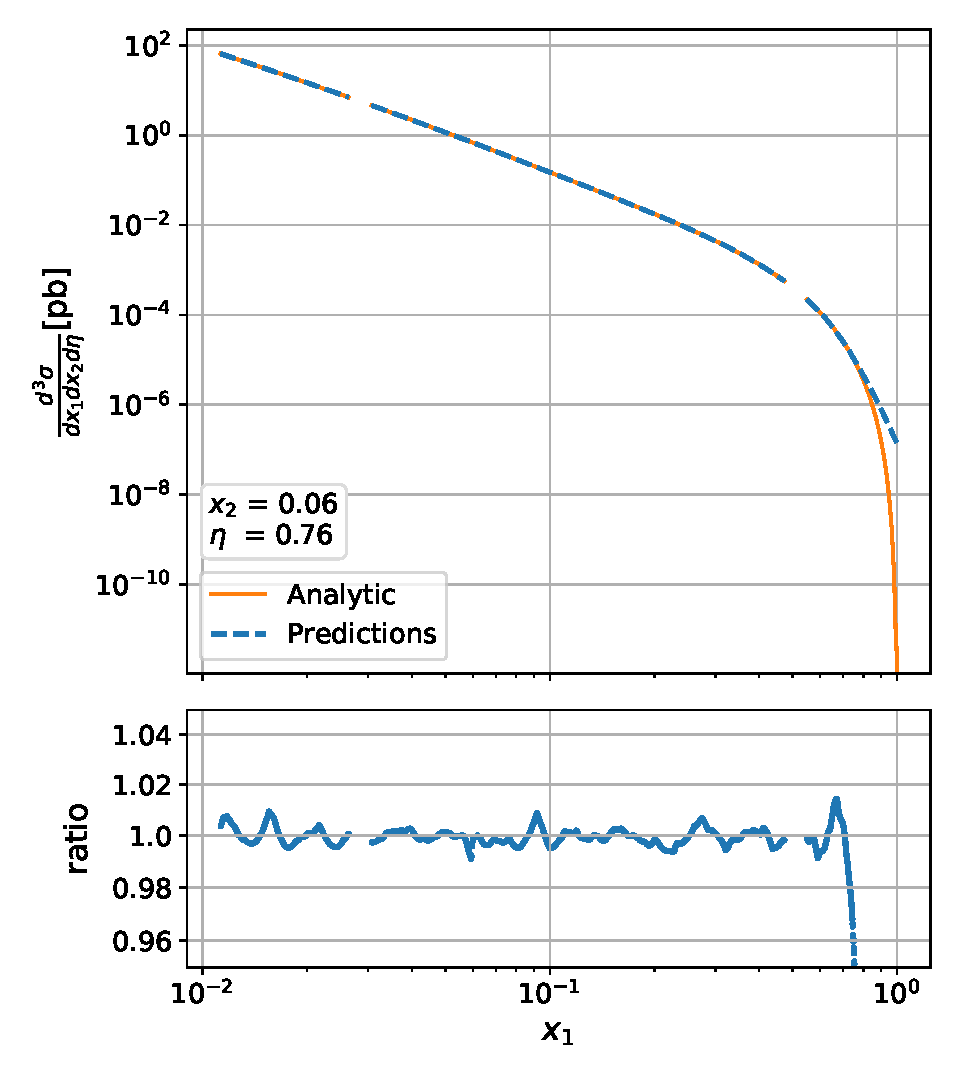
\includegraphics[width=6cm]{graphics/6}} 
	\subfloat[Schnitt in $x_1$, $x_2$ groß]{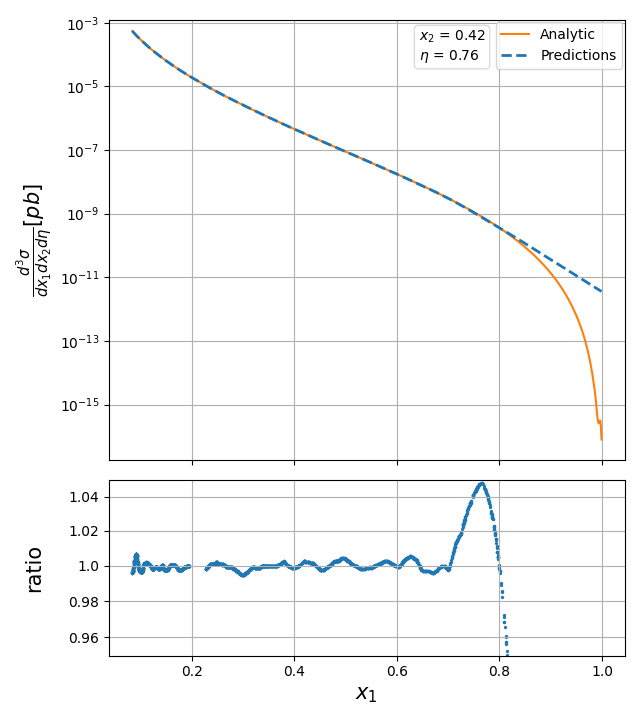
\includegraphics[width=6cm]{graphics/9}} \\
	\subfloat[Schnitt in $x_2$, $x_1$ klein]{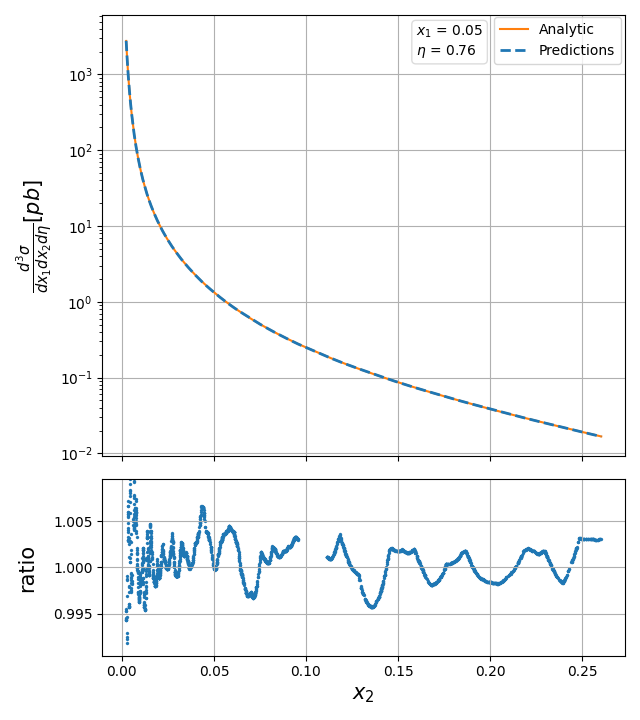
\includegraphics[width=6cm]{graphics/7}}
	\subfloat[Schnitt in $x_2$, $x_1$ groß]{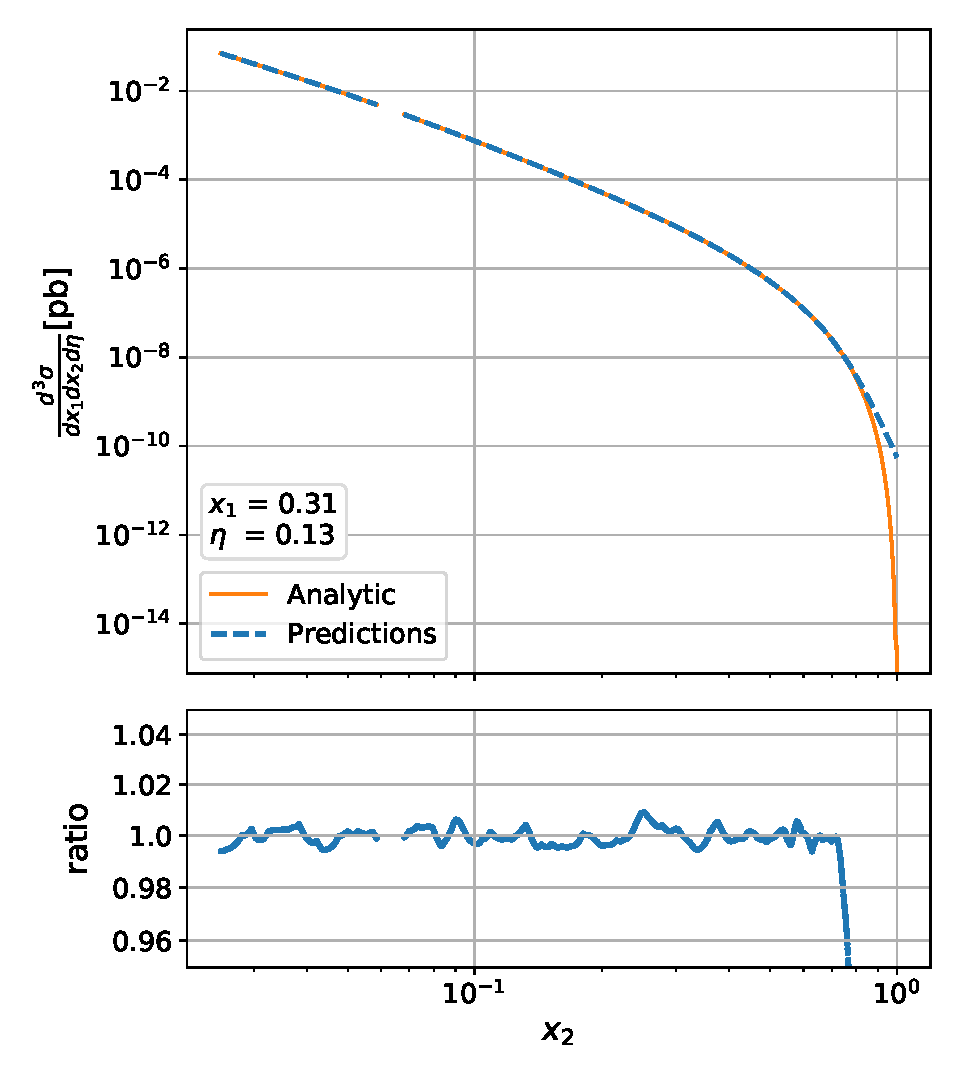
\includegraphics[width=6cm]{graphics/10}}
	\caption{Schnitte des differentiellen Wirkungsquerschnitts in $x_1, x_2, \eta$}
\end{figure}
\\
In den Abbildungen \textit{\autoref{text}}, \textit{\autoref{text}},... sind Schnitte des dreidimensionalen Wirkungsquerschnittes an verschiedenen Phasenpunkten gezeigt. Wir sehen, dass sich unsere intensive Behandlung der Hyperparameter und der Daten-Transformationen bezahlt gemacht hat. Wir verzeichnen an den meisten Stellen eine maximale Abweichung von lediglich $0.5\%$. Für Ausnahmefälle beträgt die Abweichung bis zu $\approx 1\%$. Es lässt sich leicht der Moment erkennen, ab dem die x-Werte gefiltert wurden. Wie schon im Modell für $\frac{d\sigma}{d\theta}$, verläuft die Vorhersage des Modells linear weiter und entfernt sich somit von den analytischen Werten. Für große $x$ wird unser Modell also den Wirkungsquerschnitt gegebenenfalls um Größenordnungen überschätzen. Da jedoch nur der integrierte Wirkungsquerschnitt über $x_1, x_2$ überhaupt messbar ist und dieser sich nicht merklich durch diese Abweichung beeinflussen lässt, ist die große Abweichung in diesem Phasenraumbereich vernachlässigbar. 
\subsection{Vergleich von Hyperparametern}
Wir wollen nun noch einmal direkt die Auswirkungen der einzelnen Hyperparameter an unserem Problem untersuchen. Dafür benutzen wir die Konfiguration, die wir im Vorhergehenden durch den Random Search gefunden haben und variieren für jedes Training nur einen Hyperparameter. Da die Anzahl an Neuronen und Layern stark korreliert ist, vergleichen wir auch verschiedene Architekturen. Die Modelle werden nach dem MAPE eines Test-Datestets beurteilt, das genauso gesampelt ist wie die Trainingsdaten. Wir trainieren jedes Modell fünf mal mit zufälligen Initialisierungen an zwei Millionen gesampelten Phasenraumpunkten, um die statistische Schwankung der Güte des Modells einschätzen zu können. Die eingezeichneten Fehlerbalken sollen die Schwankung verdeutlichen und sind kein Maß dafür, welchen MAPE das Netz in der Praxis erreichen kann. Ausreißer sind aus den Messungen herausfiltert, um die Skalierung in sinnvollem Rahmen zu halten. 

\textbf{Loss-Funktion:}
In \textit{\autoref{text}} a) ist der Vergleich von drei verschiedenen Kostenfunktionen gezeigt. Für Probleme mit stark variierenden Labels setzt sich der Mean-Absolute-Error durch, da dieser nicht so sensitiv auf Ausreißer oder, in unserem Fall, Polstellen ist. Der Huber-Loss, der eine Kombination des linearen Fehlers und des quadratischen Fehlers darstellt, schlägt sich insgesamt besser als der reine quadratische Fehler, kann insgesamt jedoch nicht mit dem linearen Fehler mithalten. 
\begin{figure}[t!]
	\centering
	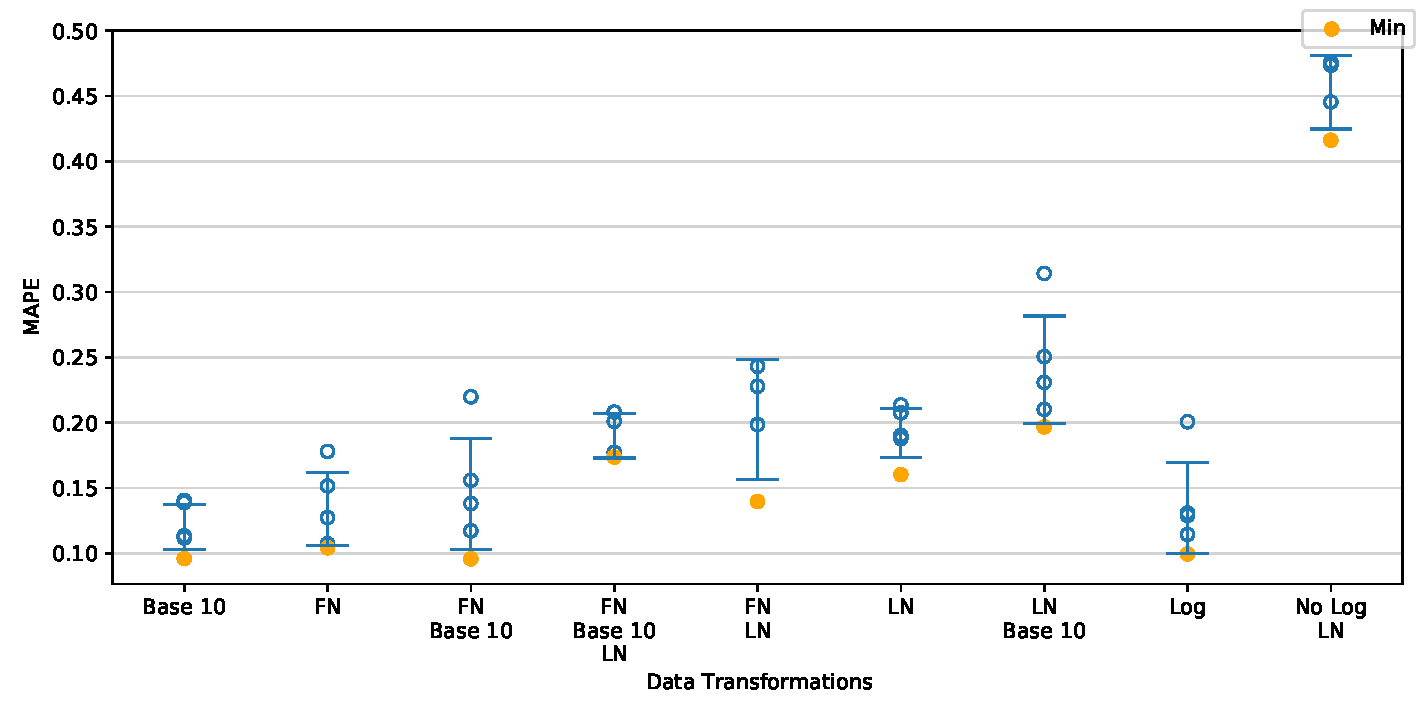
\includegraphics[width=14cm]{graphics/17,18}
	\caption{wichtig: die Daten-Transformationen ohne die überhaupt nichts geht}
	\label{besserjetzt}
\end{figure}

\textbf{Optimizer:} Der Vergleich des Optimizers \textit{\autoref{text}} c) überrascht, da generell der Adam-Optimizer in Literatur und auch erfahrungsgemäß die besten Ergebnisse liefert. RMSprop lierfert hier konstant etwas bessere Ergebnisse, wobei man jedoch beachten muss, dass bei solchen kleinen Abweichungen fünf Trainingsläuft nicht genug sind, um zu beurteilen welcher Optimizer nun besser beeignet ist. Der normale Stochastic-Gradient-Descent erzielt signifikant schlechtere Ergebnisse. 

\textbf{Trainingsdaten:}
Die Größe des Sets an Trainingsdaten ist in \textit{\autoref{text}} e) verglichen. Wie erwartet nimmt der Fehler des Modells mit der Zahl an vorhandenen Trainingsdaten ab. Das gleiche gilt voraussichtlich für die Unsicherheit auf dem Ergebnis, auch wenn in unserem Fall das Modell, das mit den meisten Trainingsdaten einen Ausreißer zeigt. Man erkennt jedoch auch, dass die Performance des Modells konvergiert und mehr als vier Millionen gesampelte Daten keinen signifikanten Beitrag mehr leisten. 

\textbf{Learning-Rate:}
An dem Vergleich der Learning-Rates, der in \textit{\autoref{text}} gezeigt ist, kann man ein interessantes Verhalten des Netzes erkennen. Für eine Learning-Rate von $1 \cdot 10^{-3}$ verändert sich der mittlere Fehler so gut wie überhaupt nicht, woraus wir schließen können, dass wir unabhängig von unserer Initialisierung bei dieser Learning-Rate das gleiche lokale Minimum finden. Die Unsicherheit der Performance wird danach mit der Learning-Rate größer, wir finden nun höhere und tiefere lokale Minima. Bei einer zu kleinen anfänglichen Lernrate, bleiben wir schon früh in einem hohen Minima stecken. Es kann daher gut sein kann, seine anfängliche Learning-Rate etwas größer zu initialisieren, als man intuitiv für richtig halten würde, da man so diversere lokale Minima finden kann. Beachte jedoch, dass dieser Ansatz nur in Kombination mit einem Zeitplan zur Reduzierung der Lernrate funktioniert und dass \grqq Dying-ReLU\glqq-Problem verstärken oder sogar auslösen kann. 

\textbf{Daten-Transformationen:}
Welche Daten-Transformationen für unser Problem funktionieren, ist in \textit{\autoref{text}} gezeigt. Ich möchte an dieser Stelle noch einmal die Wichtigkeit dieser Transformationen hervorheben. Während man in der Literatur viel über die Normalisierung oder das Reskalieren der Features liest, werden die Labels oft von Transformationen ausgenommen. Für spezielle Regressionsprobleme, wie es bei uns vorliegt, können diese jedoch der Schlüssel dazu sein, überhaupt konvergierende Modelle zu erhalten. \textit{\autoref{text}} zeigt, dass verschiedene Implementationen brauchbare Ergebnisse liefern und es wichtiger ist, überhaupt die Skalierung und den Logarithmus anzuwenden. Trainingsläufe ohne Skalierung, noch Logarithmus sind nicht aufgeführt, da der Fehler nicht vergleichbar ist. \\
\begin{figure}[bt]
	\centering
	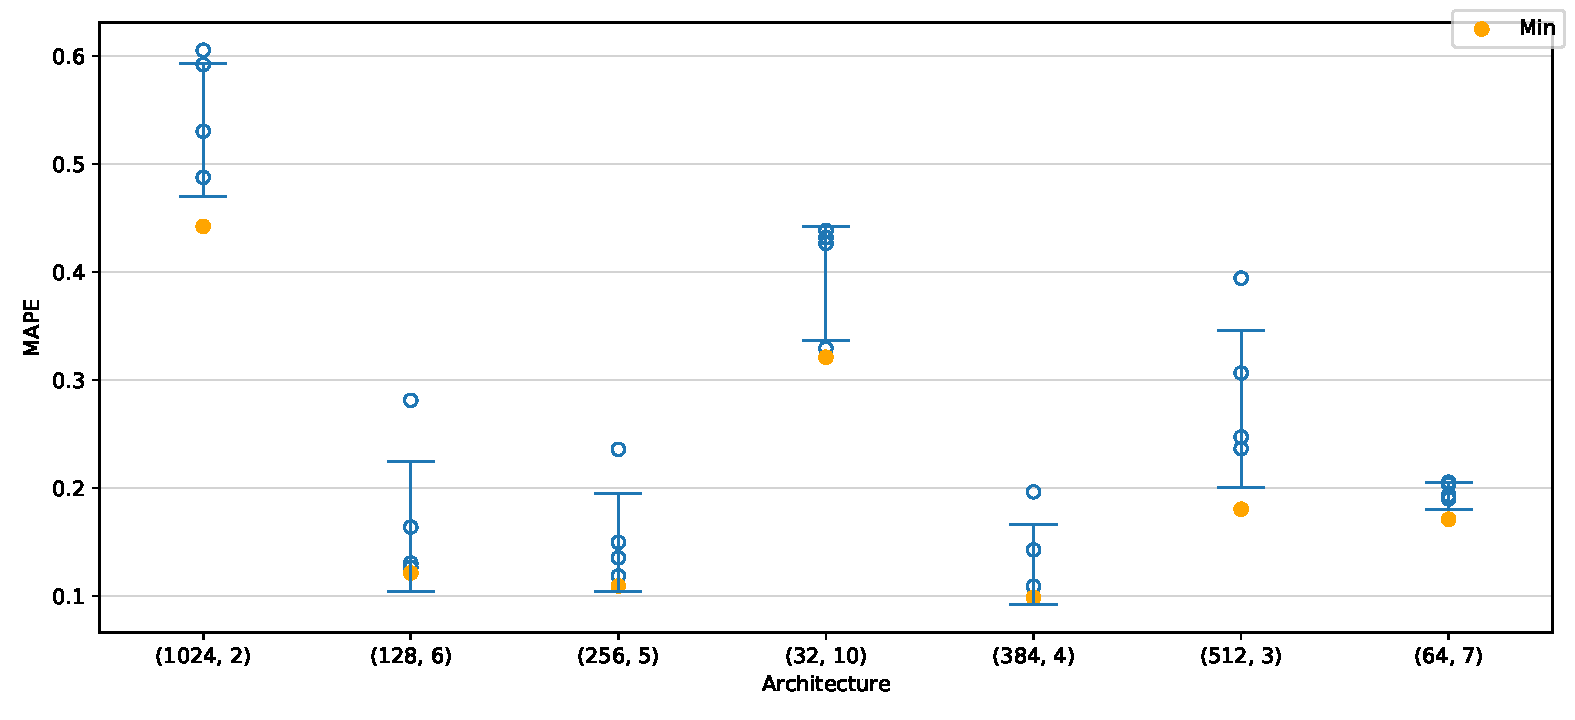
\includegraphics[width=13cm]{graphics/33}
	\caption{Vergleich für verschiedene Modell-Architekturen.
		x-Labels in (Units, Nr of Layers)}
\end{figure}

\textbf{Achitektur:} %TODO nr of layers ist nr der hidden layers ohne output oder normalisierung
Die Architektur in \textit{\autoref{text}} zu vergleichen ist interessant, da man sehen kann, dass eine passende Architektur zum Problem effektiver ist als die Komplexität des Modells. Das Modell mit den wenigsten zu trainierenden Parametern zeigt im Vergleich bessere Leistung als das komplexeste Modell. Die Modelle (128, 6), (256,5), (384, 4) zeigen unabhängig von ihren trainierbaren Parameter sehr gute Genauigkeit. Beachte jedoch, dass die rechnerische Effizienz nicht nur von der Anzahl an freien Parametern abhängt. 
% TODO trainable params unter die Architektur der Modelle

\textbf{Anzahl an Layer und Units pro Layer:} %TODO 64 als erstes bei units dann sieht es aus wie kurve
Sowohl für die Anzahl an Layer und der Units pro Layer verläuft nach einer Kurve, die ihr Minimum bei unseren optimalen Parametern hat. Der Schritt zum jeweils simpleren Modell ist klein und kann bei Bedarf einen Kompromiss zwischen Geschwindigkeit und Genauigkeit darstellen. 

\textbf{Aktivierungsfunktionen:} %TODO Link zu den Abbildungen hier?
Die Abwandlungen der ReLU-Funktion zeigen sehr gute Ergebnisse, einsehbar in \textit{\autoref{text}}. Die gewöhnliche ReLU zeigt jedoch schlechtere Leistung. Eine plausible Erklärung hierfür liefert wiederum das \grqq Dying ReLU\grqq-Problem in Kombination mit unserer vergleichsweise hohen anfänglichen Lernrate.  

\textbf{Batch-Sizes:}
Ein Trainingsvorgang ist bei größerer Batch-Size (siehe \textit{\autoref{label}}) mit passender Hardware zwar schneller, zeigt jedoch eindeutig größere Abweichungen. Aufgrund von zu wenigen Messdaten ist nicht klar, ob ein Modell, das mit großen Batches trainiert wird, in der gleichen Zeit, oder überhaupt, so tiefe Minima wie die kleineren erreichen können. 
\begin{figure}[tbp] %TODO Momentum irgendwo hinschreiben
	\centering
	\subfloat[Vergleich für verschiedene Loss-Funktionen]{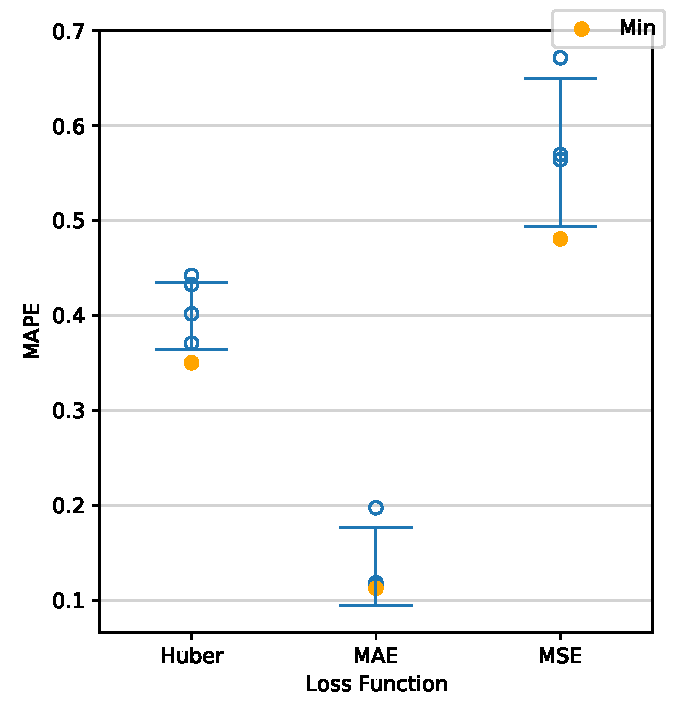
\includegraphics[width=4.5cm]{graphics/12}}
	\subfloat[Vergleich für verschiedene Zahlen an Layern]{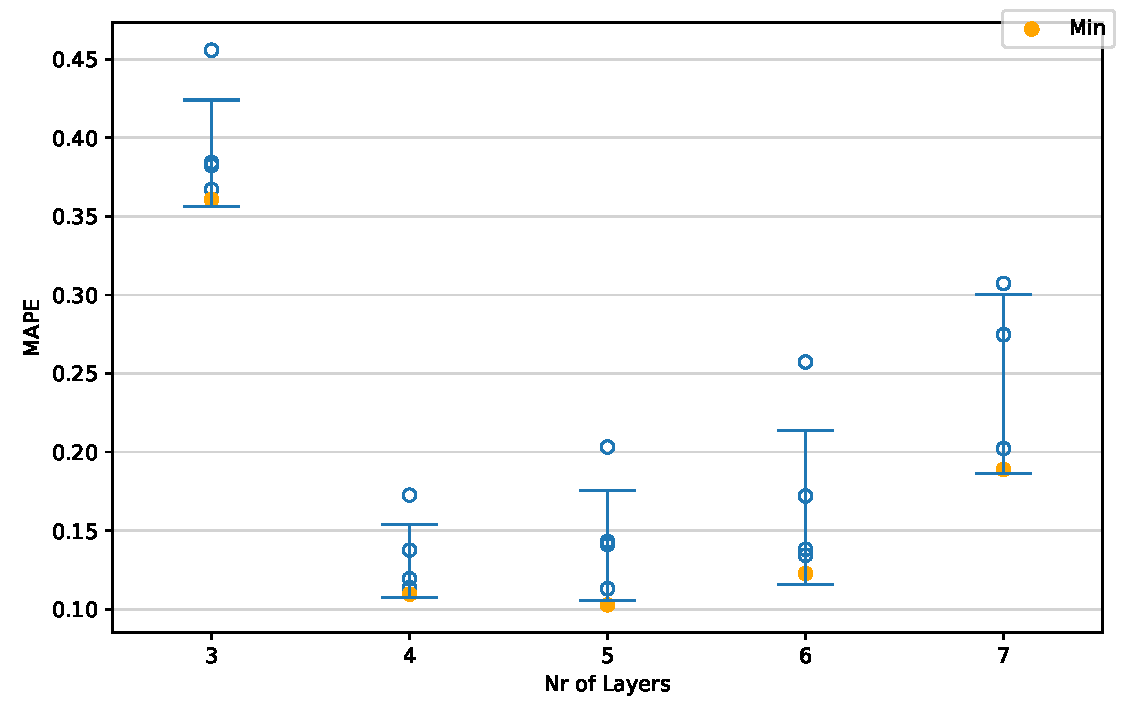
\includegraphics[width=7cm]{graphics/14}}\\
	\subfloat[Vergleich für verschiedene Optimizer]{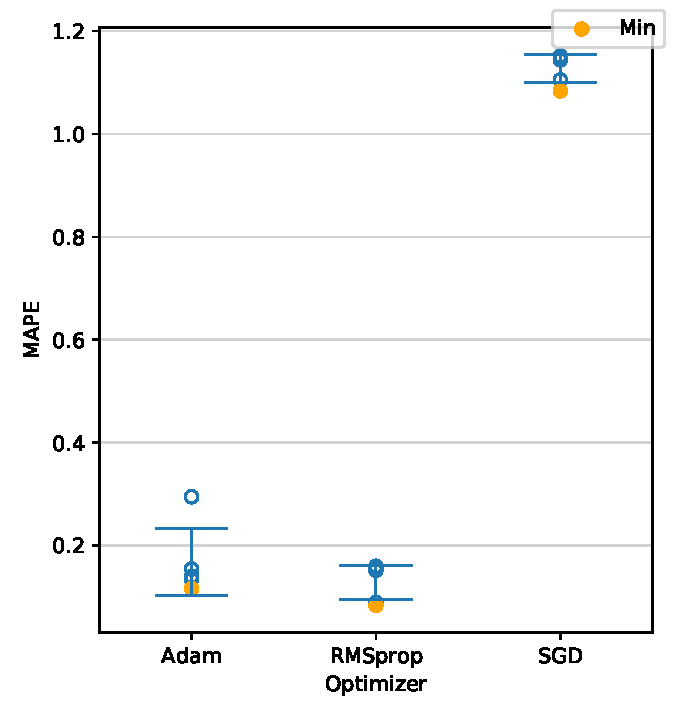
\includegraphics[width=4.5cm]{graphics/13}} 
	\subfloat[Vergleich für verschiedene Zahlen an Units]{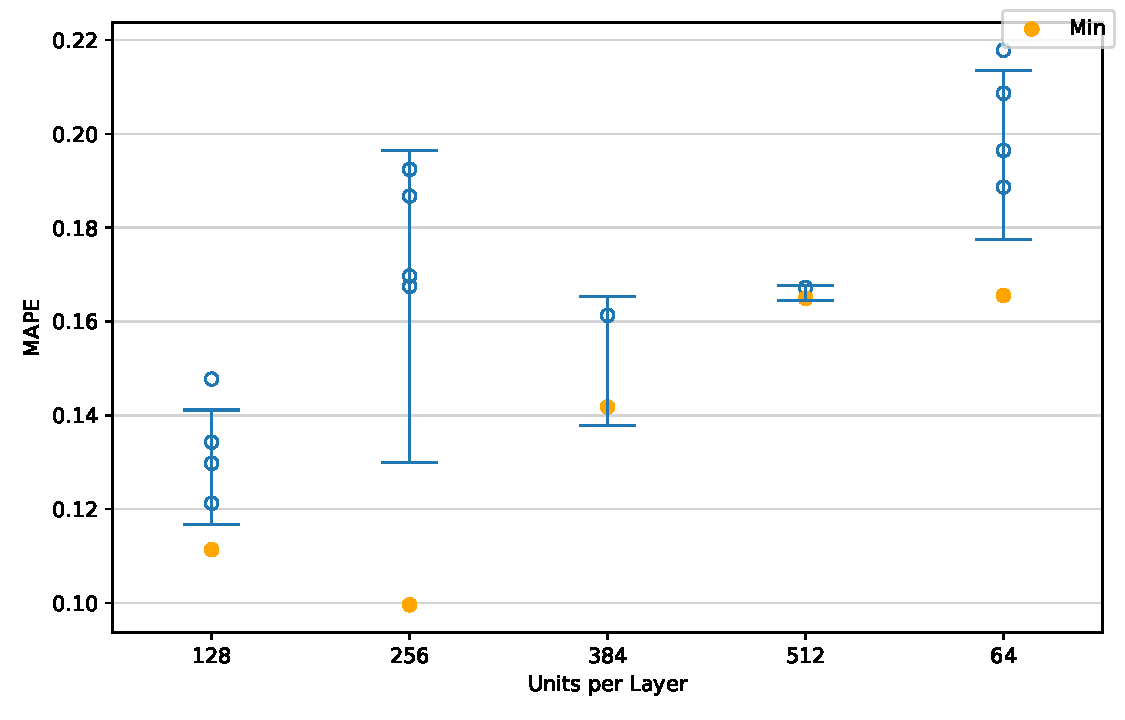
\includegraphics[width=7cm]{graphics/15}} \\
	\subfloat[Vergleich für verschiedene Anzahl an Trainigspunkten]{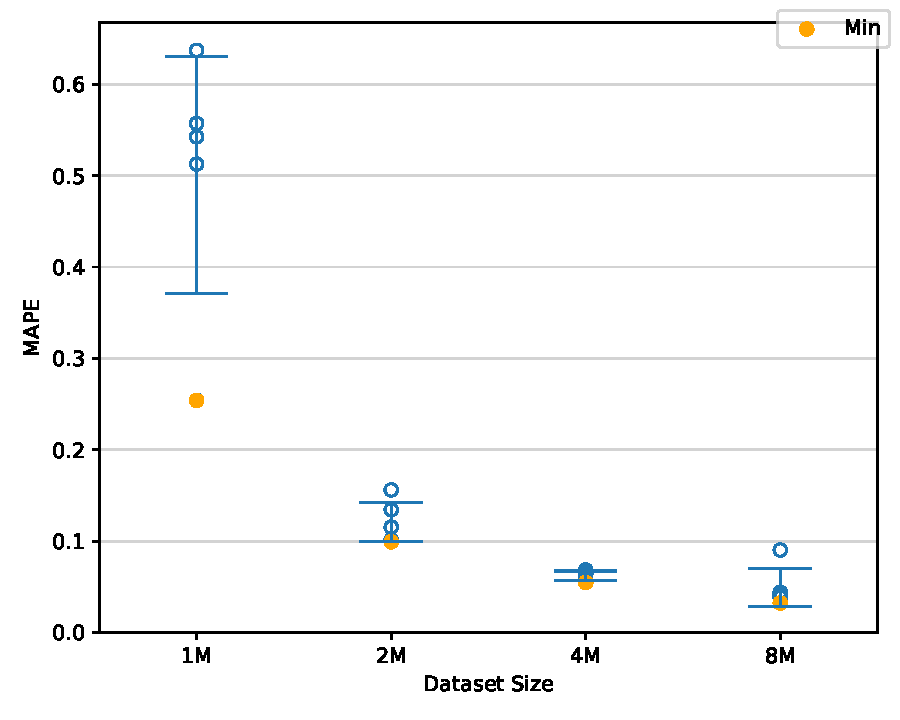
\includegraphics[width=5.75cm]{graphics/16}}
	\subfloat[Vergleich für verschiedene Anfangs-Lernraten]{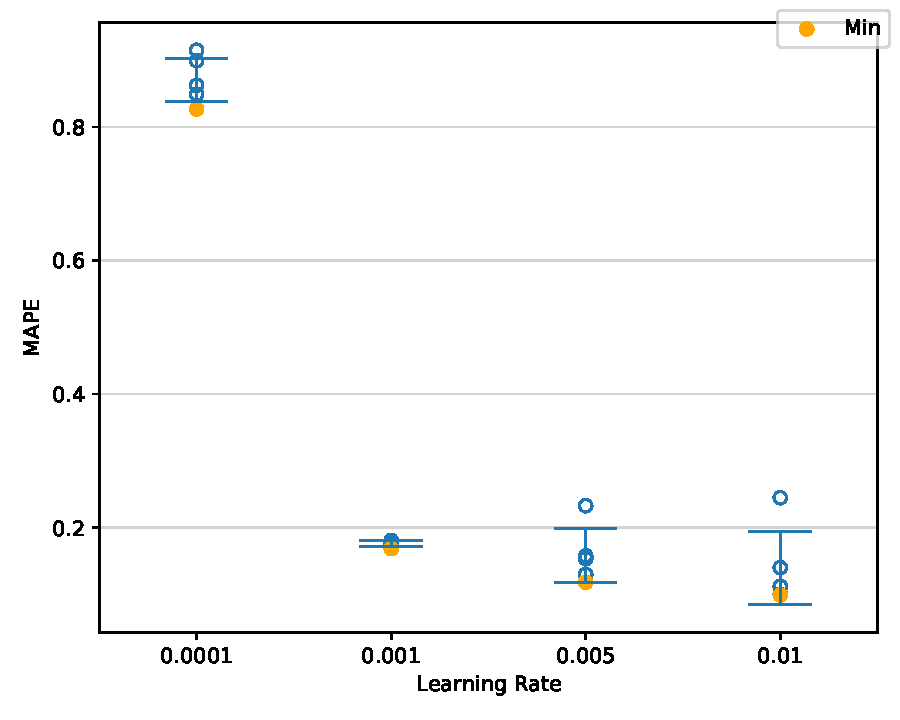
\includegraphics[width=5.75cm]{graphics/36}} 
	\caption{Vergleich von Hyperparametern (I)}
	\label{12,13,16,36}
\end{figure}
\begin{figure}[tbp]
	\centering
	\subfloat[Vergleich für verschiedene Activation-Functions]{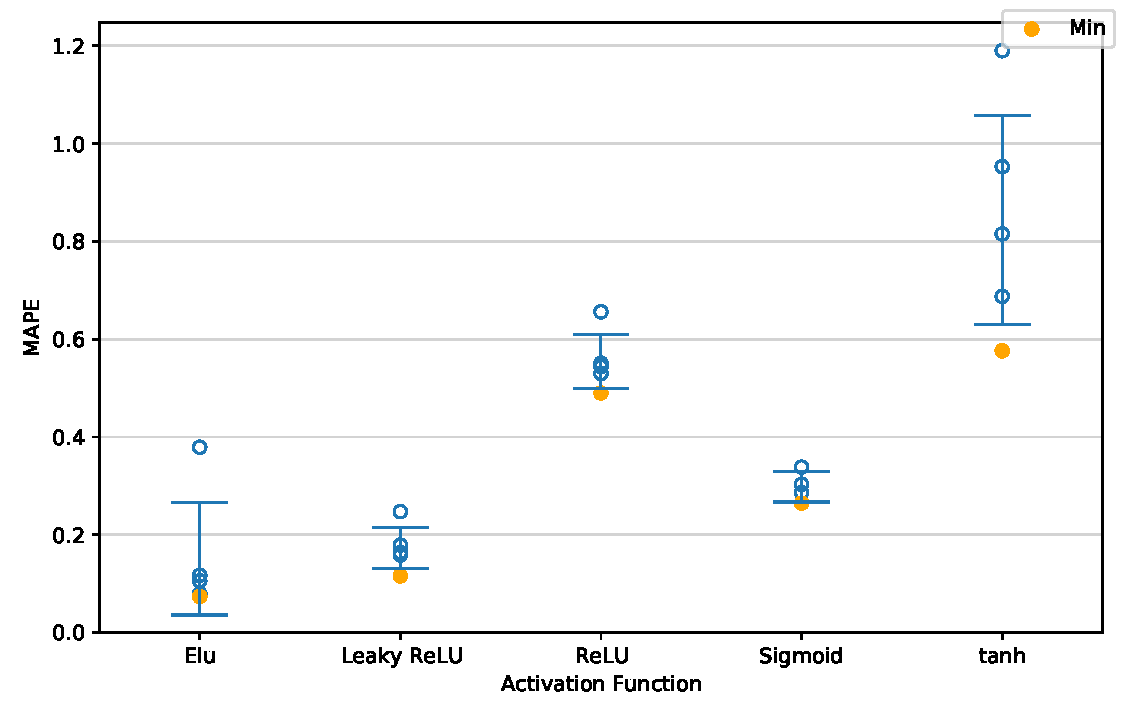
\includegraphics[width=7cm]{graphics/19}}
	\subfloat[Vergleich für verschiedene Batch-Sizes]{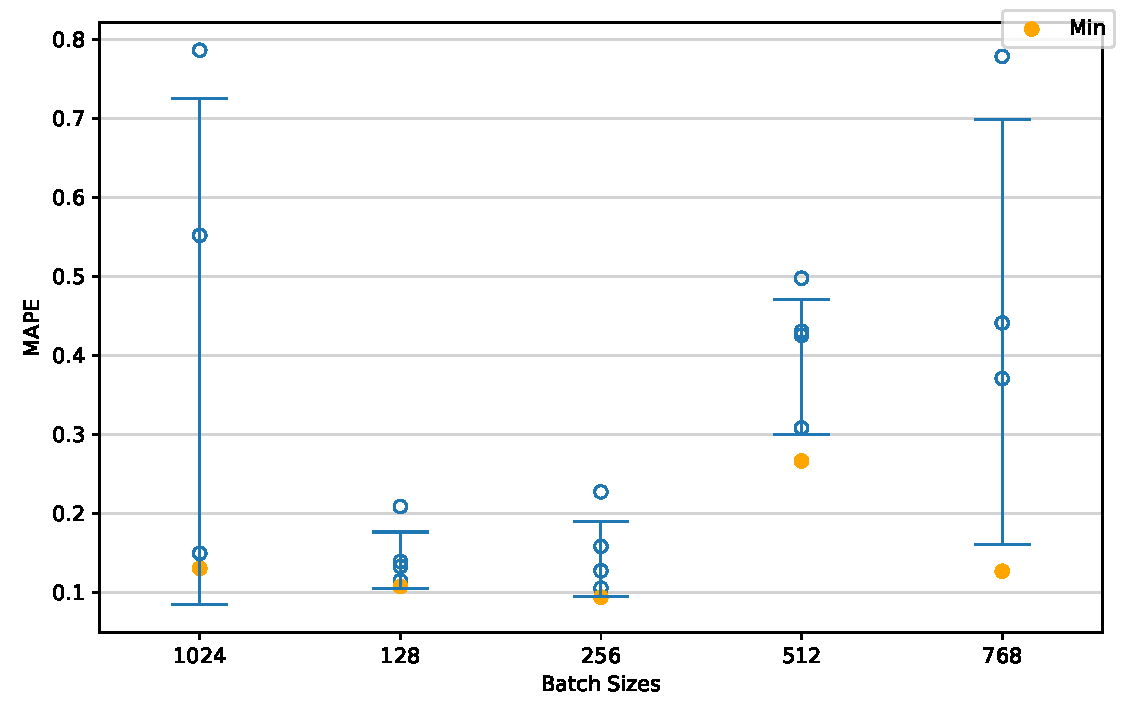
\includegraphics[width=7cm]{graphics/20}}
	\caption{Vergleich von Hyperparametern (II)}
	\label{14,15,19,20}
\end{figure}
\section{Reweight zwischen Fits der PDF}
Als nächstes möchten wir ein neuronales Netz verwenden, um die Reweights (\textit{\autoref{label}}) zwischen Wirkungsquerschnitten, die mit verschiedenen Anpassungen der PDFs berchnet wurden, zu lernen. Explizit verwenden wir im Folgenden die Fits glqq CT14nnlo\grqq~und \glqq MMHT2014nnlo\grqq~. Die Reweights schwanken um eins und haben keine Polstellen oder Ähnliches und sind damit bereits numerisch in einem geeigneten Bereich. In Phasenraumbereichen mit großen $x$ weichen die Fits jedoch stark voneinander ab und die Gewichte beginnen teils zu oszillieren. Angelehnt an den Phasenraumschnitt aus \textit{\autoref{label}}, trainieren wir die Reweights bis zu $x_{max} = 0.8$, da die starken Abweichungen etwas später beginnen. 
\\
Der Random-Search mit den besten Parametern ist in \textit{\autoref{text}} zu sehen.
\\
Wie erwartet, ist die Genauigkeit des Modells sehr gut, wie wir in \textit{\autoref{text}} beobachten können. Die Abweichung beträgt generell weniger als $0.1\%$ und ist somit kaum von den analytisch berechneten Werten zu unterscheiden. Wie das gelernte Reweight in der Praxis funktioniert, ist in \textit{\autoref{text}} dargestellt. Auch hier können wir nur minimale Abweichungen verzeichnen. Das Ratio in \textit{\autoref{text}} c) ist wie erwartet konstant, da das Reweight nicht von $\eta$ abhängt (siehe \textit{\autoref{text}}). 
\begin{figure}[htb]
	\centering
	\subfloat[Schnitt in $x_1$]{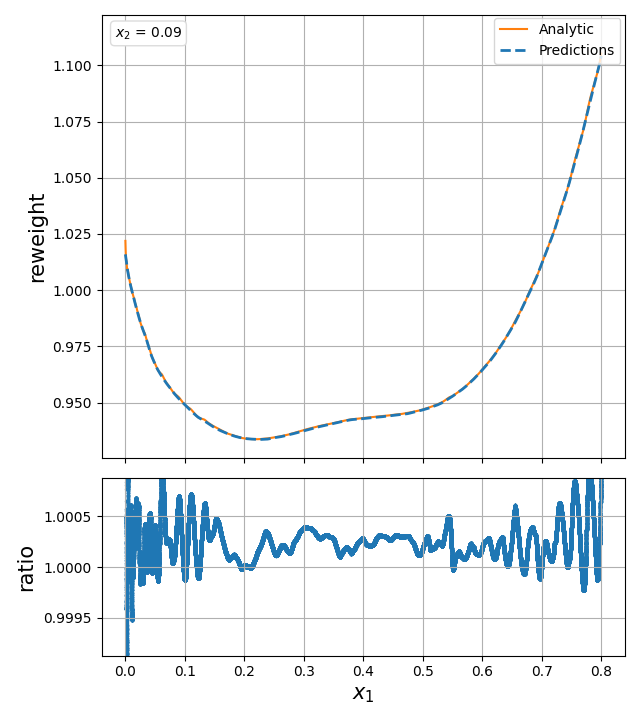
\includegraphics[width=7cm]{graphics/32}}
	\subfloat[Schnitt in $x_2$]{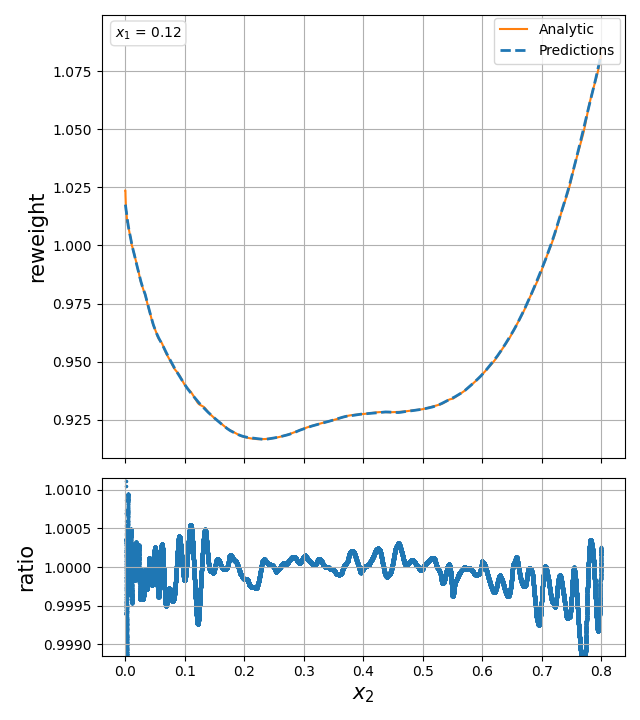
\includegraphics[width=7cm]{graphics/33_1}} 
	\caption{Vlt noch 2 3D-plots, einmal die analytischen Reweights, gelernte Reweights werden aber gleich aussehen bei der geringen abweichung}
	\label{32,33}
\end{figure}
\begin{figure}[tbp]
	\centering
	\subfloat[Schnitt in $x_1$]{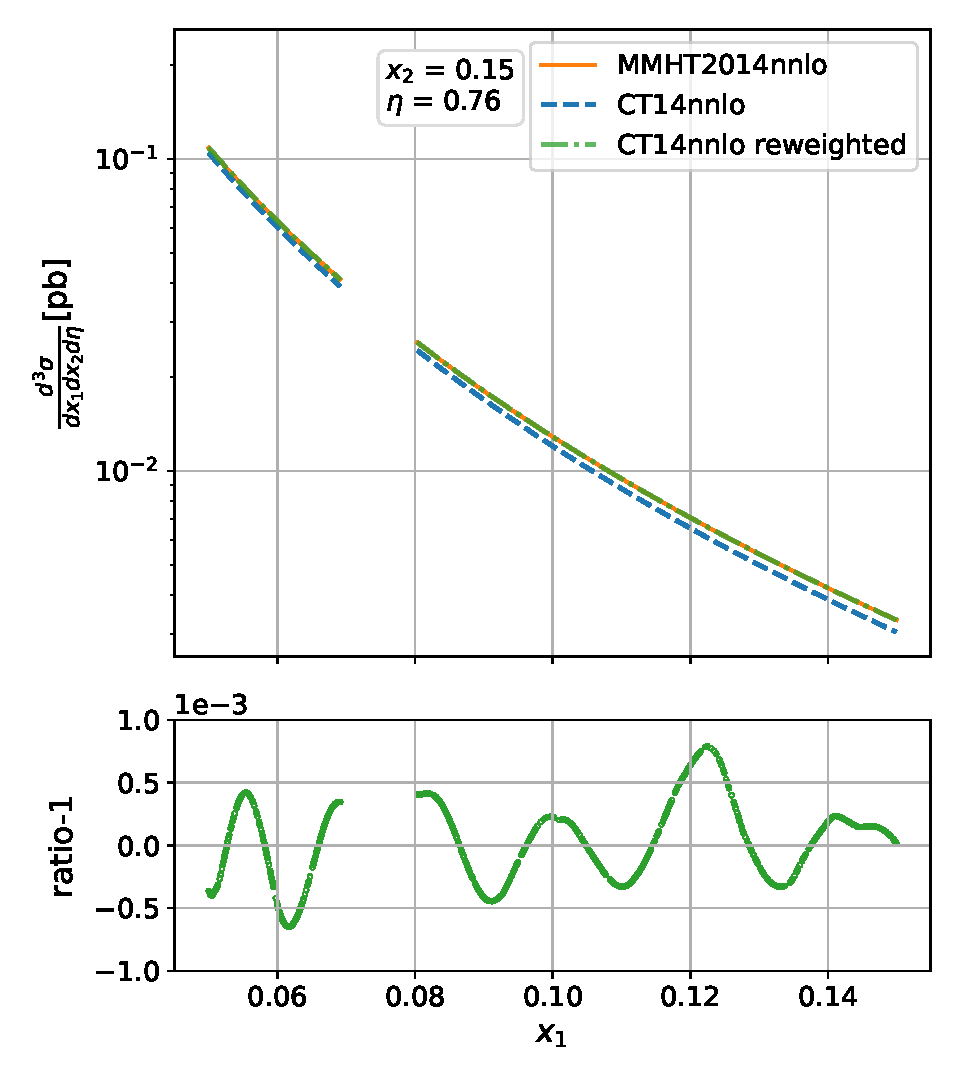
\includegraphics[width=7cm]{graphics/22}} 
	\subfloat[Schnitt in $x_2$]{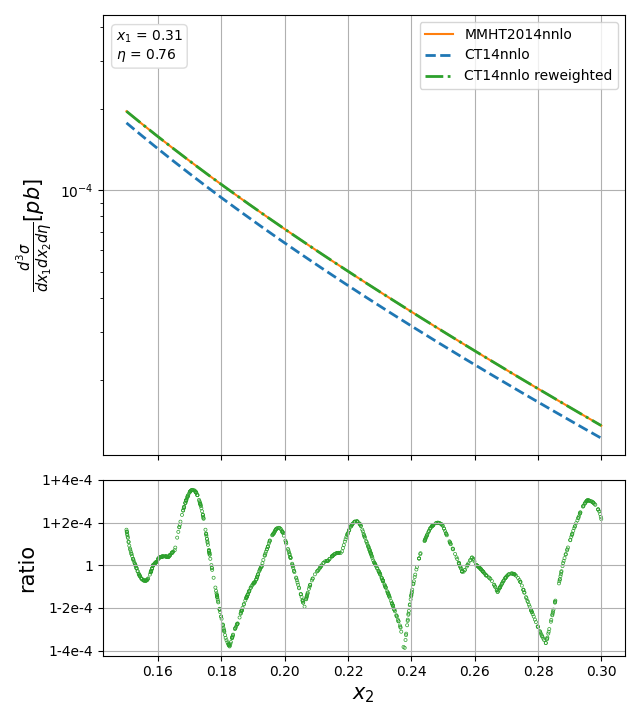
\includegraphics[width=7cm]{graphics/23.1}} \\
	\subfloat[Schnitt in $\eta$]{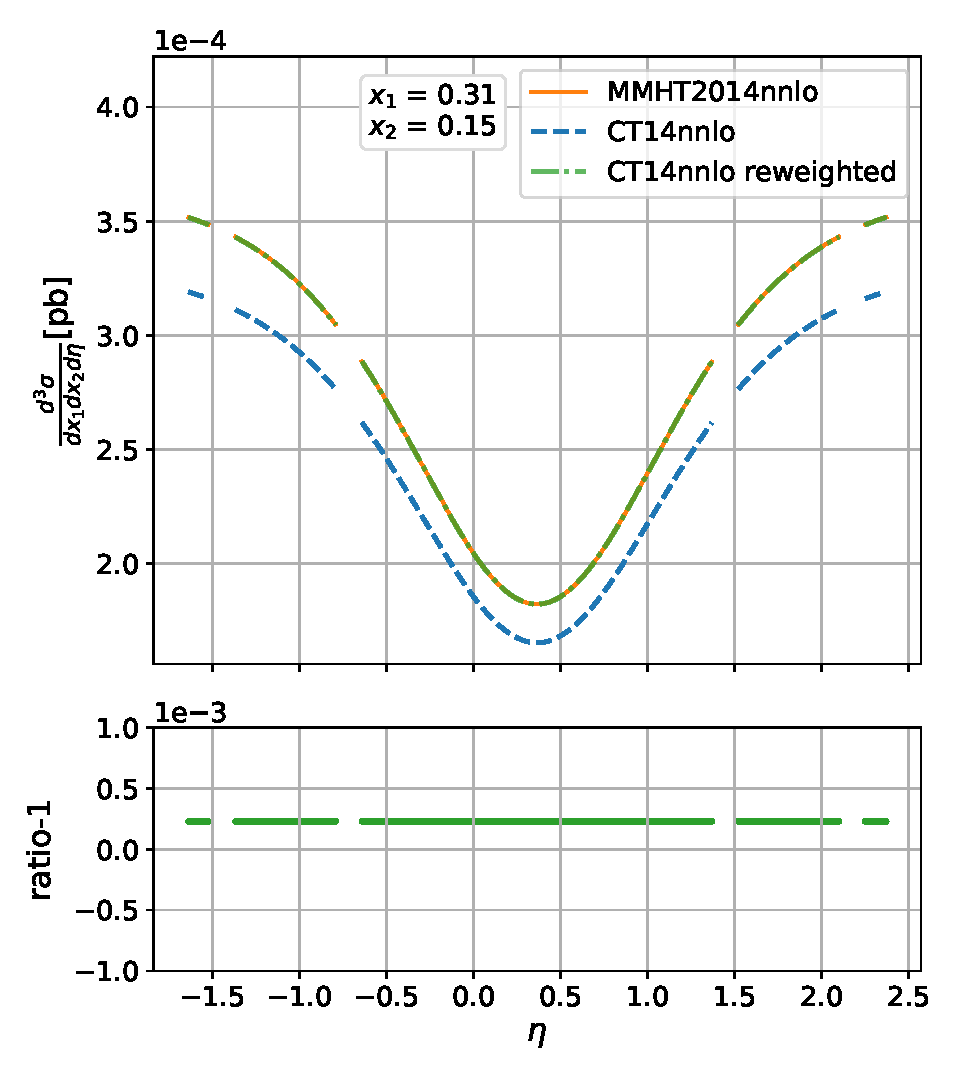
\includegraphics[width=7cm]{graphics/21}}
	\caption{Reweight von CT14nnlo auf MMHT2014nnlo mittels gelernten Weigths}
	\label{21,22,23}
\end{figure}
\section{Transfer-Learning zwischen Fits der PDF}
Eine weitere Möglichkeit, den Wirkungsquerschnitt, der mit einem anderen PDF-Set berechnet wurde, zu ermitteln, ist Transfer-Learning (siehe \textit{\autoref{}}). Mit Transfer-Learning können wir den, in den relevanten Phasenraumbereichen kleinen, Unterschied ausgleichen und mit wenig Aufwand gute Modelle für andere PDF-Fits erhalten. Wir nutzen wieder einen Random-Search, um gute Hyperparameter für den Transfer zu finden. Diese können in \textit{\autoref{label}} nachgelesen werden.\\
\\
In \textit{\autoref{label}} sind Schnitte des differentiellen Wirkungsquerschnitts mit transferiertem Modell, dem Modell das als Quelle gedient hat, und den analytischen Werten gezeigt. Wir können beobachten, dass die Genauigkeit des transferierten Modells fast identisch mit der des Source-Modells in \textit{\autoref{text}} ist. Weder verliert das Modell beim Transfer an Genauigkeit, noch beobachten wir eine Verbesserung der Performance, die dem Transfer-Learning manchmal zugesprochen wird.\\
Eindeutig können wir sehen, dass sich die Menge an Lerndaten und damit auch die Trainingsdauer stark verringert. Es konnte mit einfachen Mitteln eine Reduktion um den Faktor vier an Trainingspunkten erreicht werden. Sowohl das Transfer-Learning, als auch das Reweighting sind also legitime Methoden um den Wirkungsquerschnitt von einem PDF-Set auf das nächste zu übertragen. Ein visueller Vergleich folgt in \textit{\autoref{label}}, wobei sich hier nicht erkennen lässt, welche Methode die besseren Leistungen zeigt. Interessant zu sehen ist, dass sich die Form des Ratios beider Modelle ähnelt. Der Grund hierfür liegt darin, dass das transferierte Modell vom Source-Modell abstammt und sich die Gewichte der Nodes ähneln.\\
\\
In \textit{\autoref{text}} sind einige Eigenschaften gegenübergestellt.
\begin{table} % TODO Trainingszeit passt noch nicht so ganz
	\centering
	\begin{tabular}{|l|c|c|c|c|}
		\hline
		Modell & MAPE & Training$[\text{s}]$ & Punkte & TPM$[\text{s}]$ \\
		\hline
		Reweight + Source & 0.076 & 243.42 & 1M & 30.60 \\
		Reweight + Analy. &  0.017 & 243.42 & 1M & 13.84 \\
		Transfer & 0.204 & 85.78 & 1M & 15.73\\
		Transfer + FT & 0.064 & 164.83 & 1M & 15.65 \\
		Source-Model & 0.229 & 841.46 & 4M & 15.81\\
		\hline
	\end{tabular}
	\caption{Vergleich von Reweight- und Transfer-Modellen TPM: Time per Million, Berechnungszeit für $10^{6}$ Punkte}
\end{table}
Wir sehen, dass das präziseste und schnellste Modell das Reweighting der analytisch berechneten Werte ist. Verfügt man also bereits über eine große Anzahl an Werten von differentiellen Wirkungsquerschnitten, dann ist dies das Modell der Wahl. Möchten wir jedoch über ein vollständiges Modell verfügen, dass nicht auf die analytische Berechnung von differentiellen Wirkungsquerschnitten angewiesen ist, schneidet das Modell \glqq Transfer + FT\grqq~am Besten ab. Es sticht seinen Konkurrenten \glqq Reweight + Source\grqq~ in allen betrachtet Kriterien aus. Da im zweiten Fall sowohl die Reweights mit einem Netz, als auch die Source-Wirkungsquerschnitten mit neuronalen Netzen berechnet werden, verdoppelt sich hier die TPM im Vergleich zu den restlichen Modellen. Transferieren wir das Source-Model auf eine geeignete Art, passt sich das Netz gut an die neuen Daten an und der MAPE bleibt minimal. Gewichten wir jedoch die Ergebnisse des Source-Models neu, pflanzen sich beide Ungenauigkeiten fort und die Unsicherheit steigt etwas. \\
\\
Wir kommen zum Schluss, dass das Transfer-Learning eine generell bessere Methode für den angesprochenen Zweck ist und das Erlernen des Reweights zwar gut funktioniert, jedoch nur nützlich ist, wenn man für speziell die Gewichte benötigt.
\begin{figure}[tbp]
	\centering
	\subfloat[Schnitt in $x_1$]{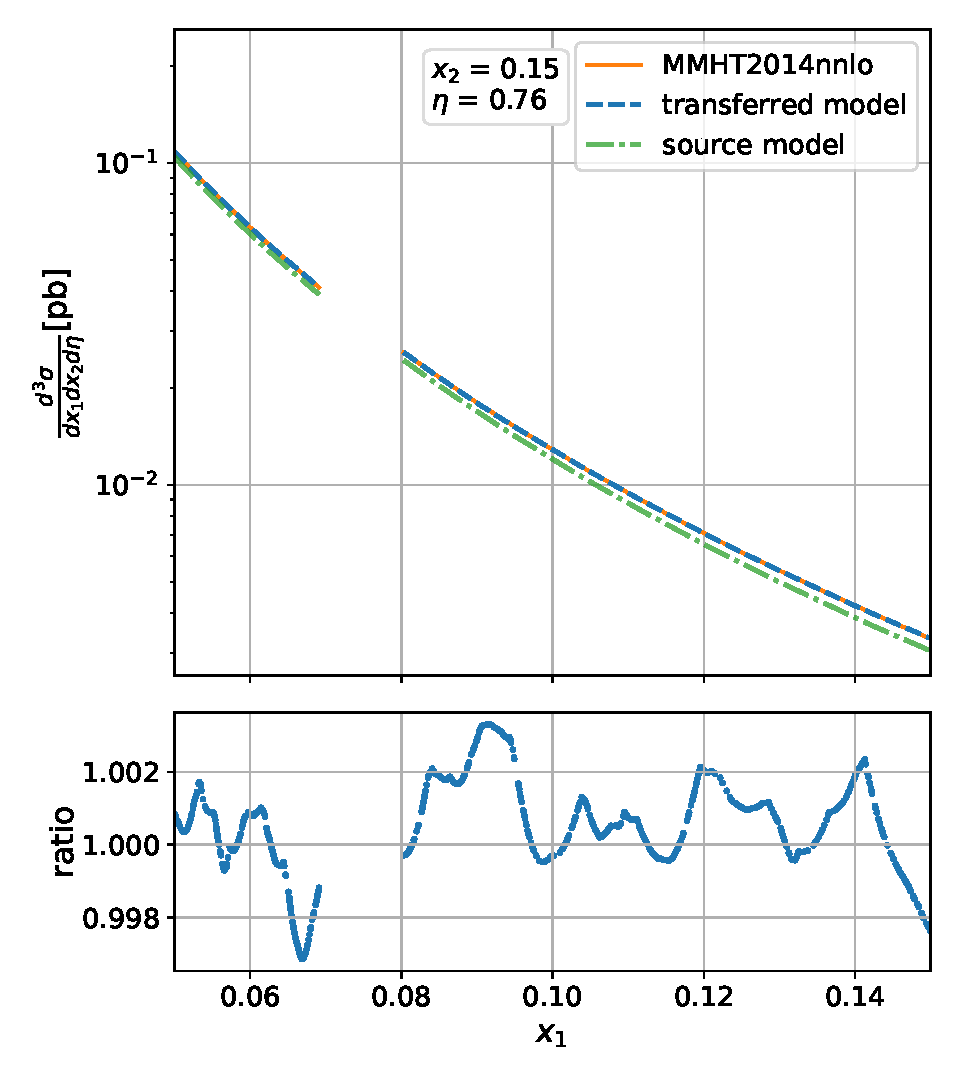
\includegraphics[width=7cm]{graphics/34}} 
	\subfloat[Schnitt in $x_2$]{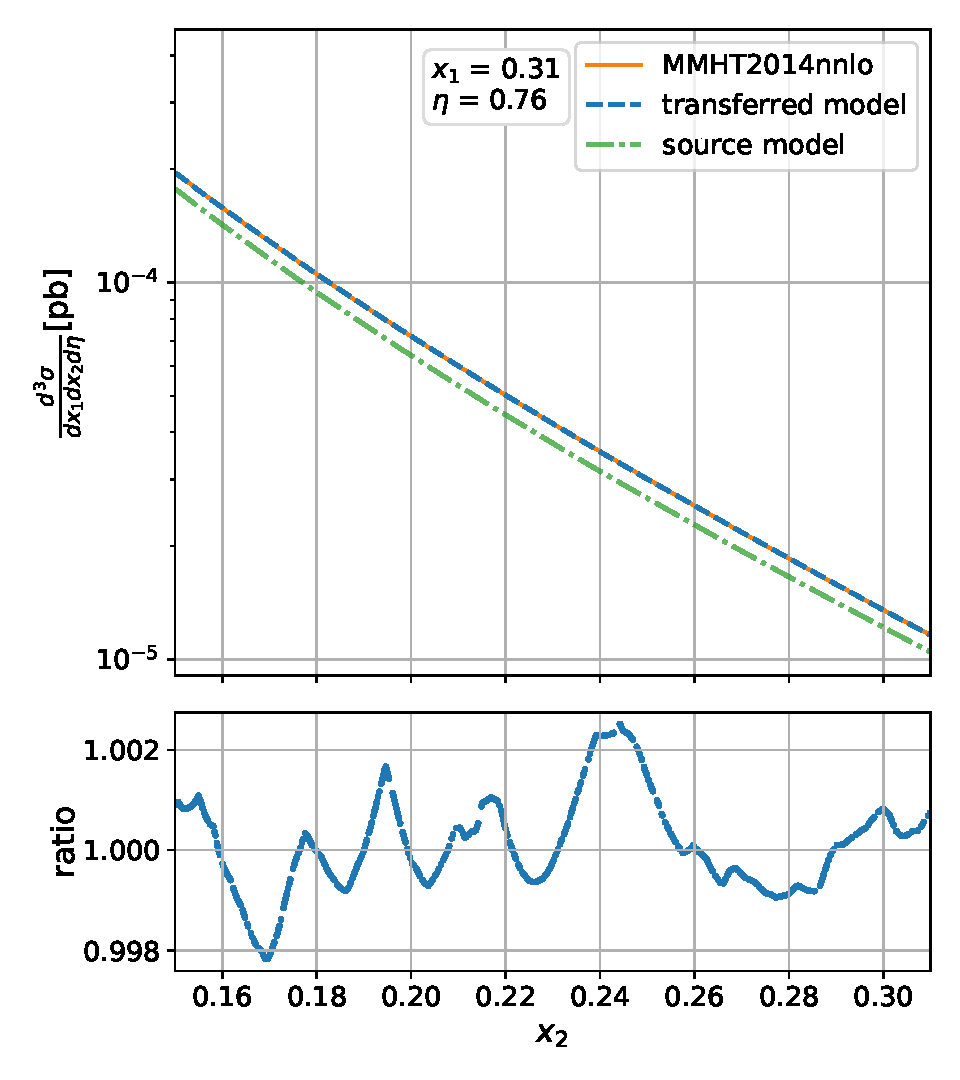
\includegraphics[width=7cm]{graphics/35.1}} \\
	\subfloat[Schnitt in $\eta$]{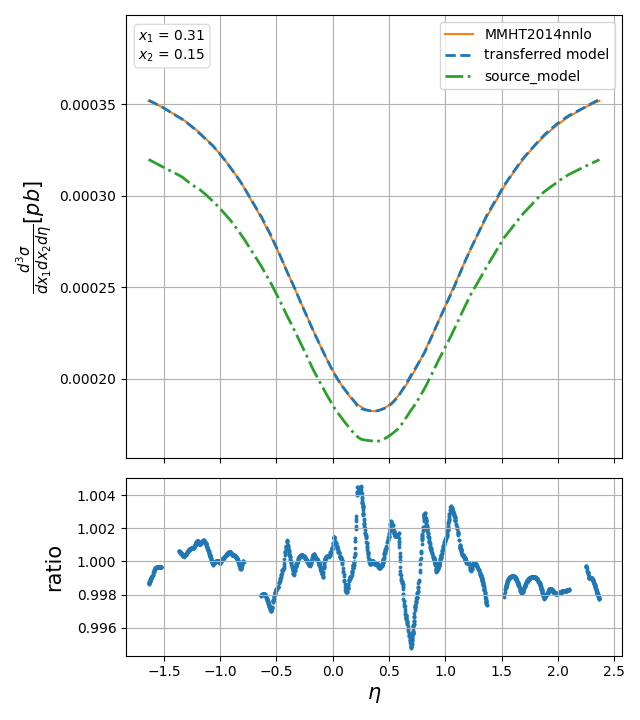
\includegraphics[width=7cm]{graphics/24}}
	\caption{Transferiertes Model von Source Model zum Transfer model}
	\label{34,35,24}
\end{figure}
\begin{figure}[tbp]
	\centering
	\subfloat[Schnitt in $x_1$]{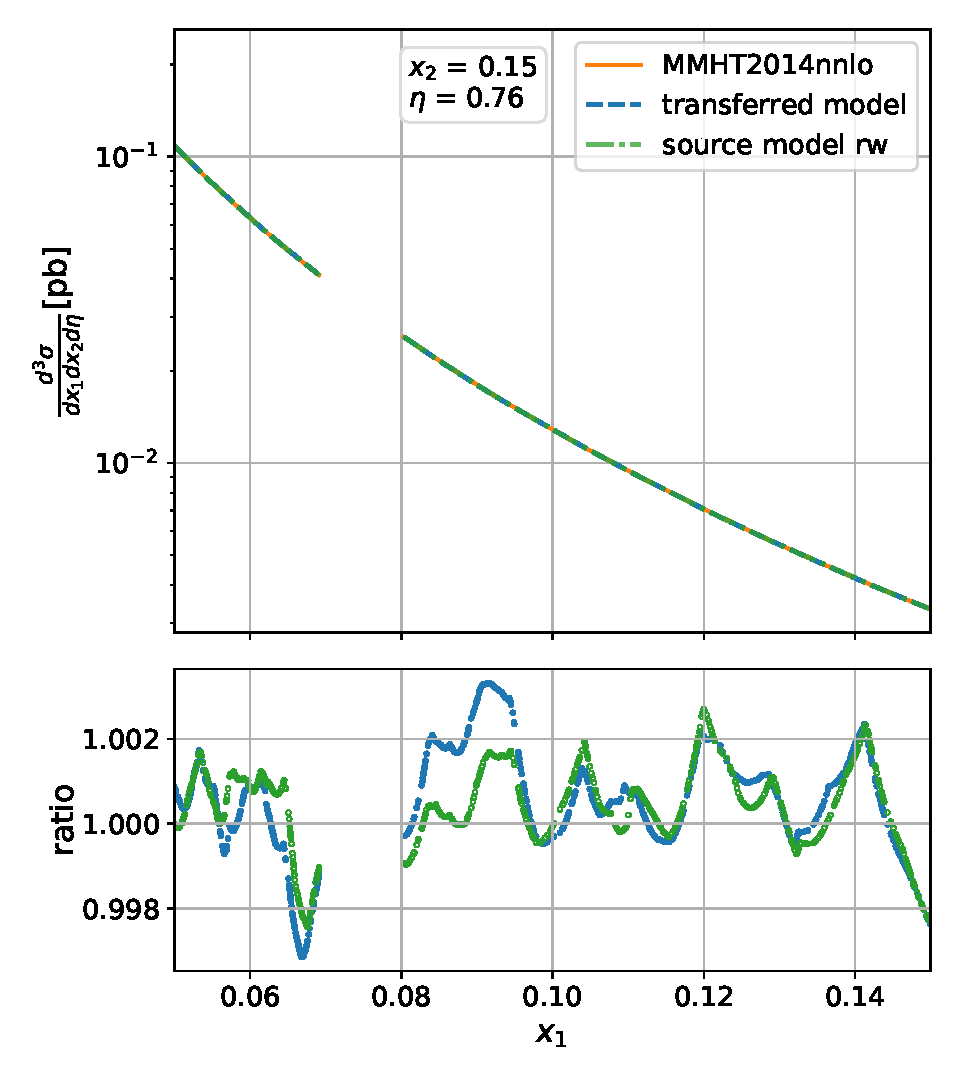
\includegraphics[width=7cm]{graphics/34.3}} 
	\subfloat[Schnitt in $x_2$]{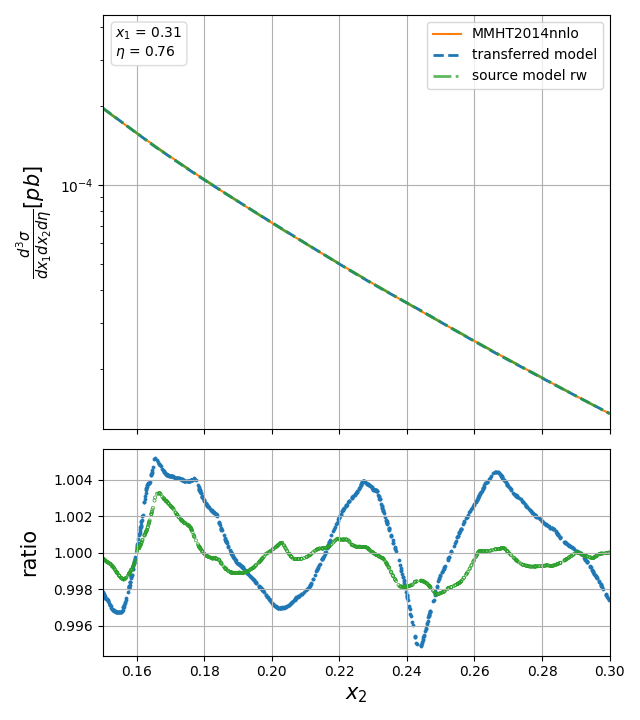
\includegraphics[width=7cm]{graphics/35.2}} \\
	\subfloat[Schnitt in $\eta$]{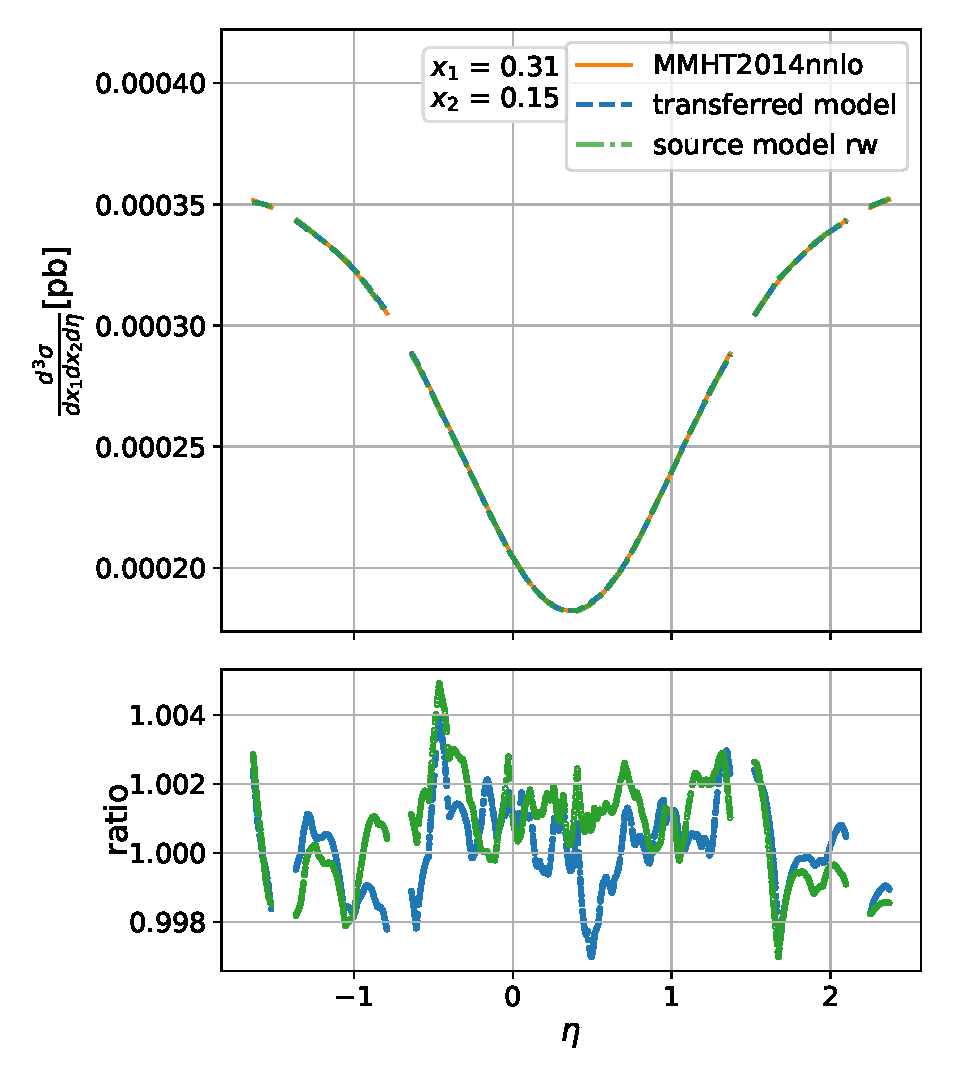
\includegraphics[width=7cm]{graphics/24.2}}
	\subfloat[Vergleich]{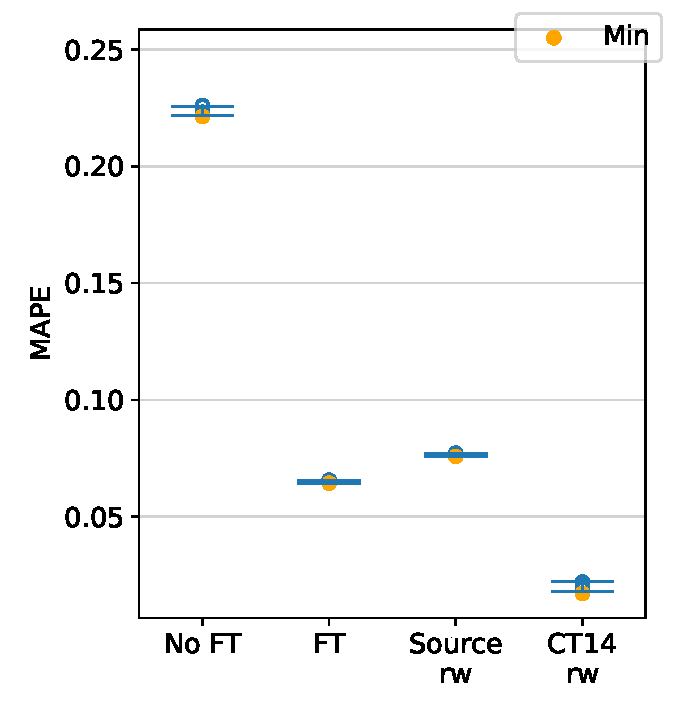
\includegraphics[width=7cm]{graphics/25,29}}
	\caption{Vergleich transferiertes Modell, gereweightetes Source Model
		rw: reweighted}
\end{figure}
\section{Monte-Carlo-Integration}
\subsection{Parton-Ebene}
Wir nutzen Monte-Carlo-Methoden zur Integration von \textit{\autoref{text}}, \textit{\autoref{text}} und deren zugehörigen Machine Learning Modellen. Zur Integration von \textit{\autoref{text}} nutzen wir das Importance Sampling aus \textit{\autoref{text}}, um die Konvergenz des Integrals zu beschleunigen. Der Prozess $qq \rightarrow \gamma \gamma$ ist zwar nicht messbar, jedoch müssen wir trotzdem einen Cut in $\eta$ festlegen, da der totale Wirkungsquerschnitt sonst divergiert. Wir entscheiden uns für die Beschränkungen \textit{\autoref{text}}.
\begin{equation}
\abs{\eta} \leq 2.5 \qquad \Rightarrow \qquad \theta \in \left[\epsilon, \pi - \epsilon \right] \quad \text{mit} \quad \epsilon = 0.1638
\end{equation}
Die Unsicherheit auf unsere Monte-Carlo-Integration bestimmen wir aus \textit{\autoref{text}}. Wir führen die Integrationen mit 1000 Stützstellen durch und wiederholen die Integration 100 mal. In \textit{\autoref{text}} sind die erhaltenen Ergebnisse mit dem analytischen Wert verglichen.
\begin{table}[bh]
	\centering
	\begin{tabular}{lll}
		Integrand & \multicolumn{2}{c}{$\quad \sigma_{\text{tot}}[\text{pb}]$} \\
		\hline
		analytische Stammfunktion& \quad  $0.053793$ &$\pm~ 0$\\
		$\derivative{\sigma}{\theta}$ analytisch + IS & $\quad 0.05382 $&$\pm~ 0.00006 $ \\
		$\derivative{\sigma}{\theta}$ analytisch & $\quad 0.05389$ &$\pm~ 0.00015 $ \\
		$\derivative{\sigma}{\theta}$ ml + IS &$\quad 0.05386$ &$\pm~ 0.00005$ \\
		$\derivative{\sigma}{\eta}$ analytisch & $\quad 0.053796 $&$\pm~ 0.000034$ \\
		$\derivative{\sigma}{\eta}$ ml & $\quad 0.053801 $&$\pm~ 0.000034$ \\
	\end{tabular}
	\caption{Monte-Carlo-Integration des partonischen Diphoton Prozesses}
\end{table}
Wir sehen, dass die neuronalen Netze so präzise sind, dass ihre Abweichung in der Unsicherheit der Monte-Carlo-Integration untergeht. Das sind gute Voraussetzungen für die Anwendbarkeit von neuronalen Netzen auch bei höherdimensionalen Prozessen. Das simple Importance-Sampling bringt eine signifikante Varianz-Verringerung mit sich.
\subsection{Hadron-Ebene}
Auch für den hadronischen Diphoton-Prozess nutzen wir Importance-Sampling. Für die Generation der Impulsbruchteile $x$ verwenden wir die Verteilung aus \textit{\autoref{text}}. Aufgrund der Cuts leisten Phasenraumpunkte mit kleinem $\eta$ einen Größeren Beitrag zum messbaren $\sigma_{\text{tot}}$, wir ziehen daher Punkte aus einer Gaußverteilung um Null($\textit{\autoref{label}}$).
\begin{equation}
\rho(\eta) = \frac{1}{\sqrt{2\pi \sigma^2}} \exp(-\frac{(\eta)^2}{2\sigma^2}) \quad \text{mit} \quad \sigma=2
\end{equation}
Wir integrieren zunächst über zwei Freiheitsgrade und sehen uns die Wirkungsquerschnitte in Abhängigkeit von $x_1, x_2$ und $\eta$ an. Wir samplen dazu 50.000.000 Punkte, mit gleicher Sample-Effizienz wie in \textit{\autoref{label}} und wiederholen den Prozess fünf mal. Die Ergebnisse sind in \textit{\autoref{label}} dargestellt.
\begin{figure}[tbp]
	\centering
	\subfloat[Integration über $x_2, \eta$]{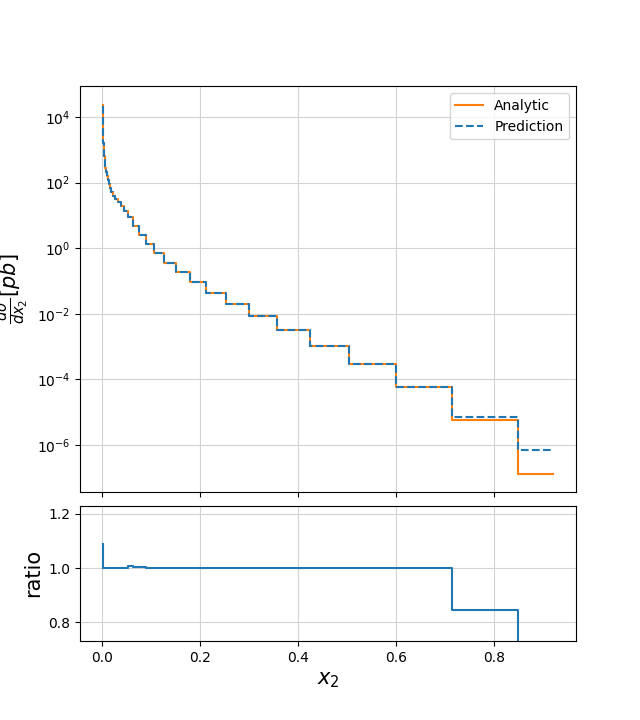
\includegraphics[width=7cm]{graphics/27}} 
	\subfloat[Integration über $x_1, \eta$]{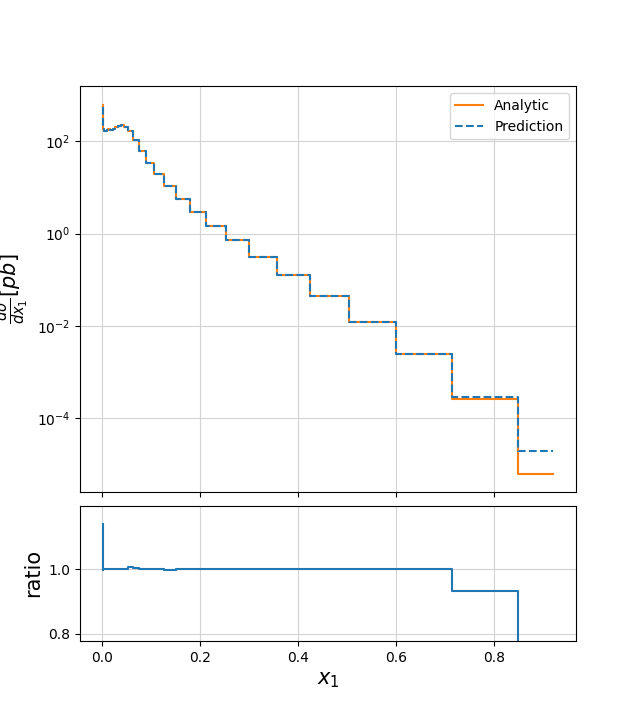
\includegraphics[width=7cm]{graphics/28}} \\
	\subfloat[Integration über $x_1, x_2$]{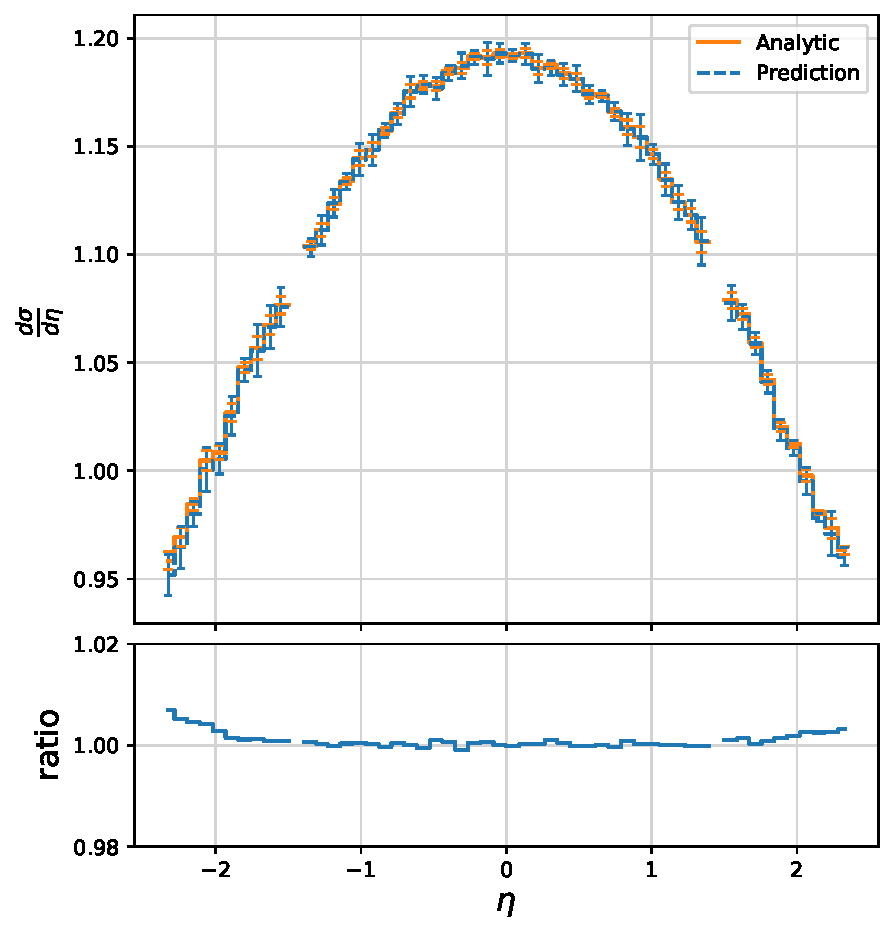
\includegraphics[width=7cm]{graphics/11}}
	\caption{MC-Integrationen über zwei Freiheitsgrade}
	\label{11,27,28}
\end{figure} %TODO sicherstellen, dass ratio immer analytisch/WQ ist.
Wie wir sehen, überdecken sich die integrieren Wirkungsquerschnitte für die analytischen Werte und die Vorhersagen des neuronalen Netzes an vielen Phasenpunkten. Lediglich für große $x$ überschätzt die Vorhersage wie erwartet den eigentlichen Wert. Diese Abweichung kann jedoch vernachlässigt werden, da wir am Ratio von \textit{\autoref{label}} c) sehen, dass die analytischen Werte insgesamt unterschätzt werden. Der Grund hierfür liegt vermutlich in der Polstelle an $x=0$. Durch die Cuts werden viele Phasenraumpunkte um $x_1 = x_2 = 0$ mit großem Wirkungsquerschnitt herausgenommen, da sie die $p_T$-Hürde nicht erfüllen und führt voraussichtlich zu einer geringfügigen Unterschätzung des Wirkungsquerschnittes an diesen einflussreichen Stellen. \\
\\
Zur Integration über alle Freiheitsgrade verwenden wir die gleichen Daten wie im vorherigen Abschnitt. Wir erhalten die Ergebnisse \textit{\autoref{label}}.
\begin{equation}
\begin{aligned}
&\sigma_{\text{tot}}^{\text{analytic}}&=  (5.1707 \pm 0.0038) \text{ pb}\\
&\sigma_{\text{tot}}^{\text{ml}} &= (5.1634 \pm 0.0038) \text{ pb} \\
\end{aligned}
\end{equation}
Dies entspricht einer Abweichung von $0.14\%$, wobei die Unsicherheiten der Monte-Carlo-Integration zusätzlich überlappen. Wir können also abschließend sagen, dass die Präzision des DNN sehr gut und die Näherung erfolgreich gelungen ist.   
\chapter{Zusammenfassung und Ausblick}
\section{Zusammenfassung}
In dieser Arbeit wurde der Diphoton Prozess als $q\overline{q} \rightarrow \gamma \gamma$ und $pp \rightarrow \gamma \gamma$ auf Leading-Order Ebene behandelt und Ausdrücke für die jeweiligen differentiellen Wirkungsquerschnitte hergeleitet. An dies Beispielen wurde dann die Eignung von tiefen neuronalen Netzwerken zur Näherung des Integranden überprüft. Dabei mussten verschiedene Tücken bedacht und behandelt werden. In diesem Kontext wurde die Wichtigkeit von Label-Transformationen und der Architektur des Neuronalen Netzes deutlich. Anschließend wurden die Gewichte zwischen den Fits der Partondichtefunktionen CT14nnlo und MMHT2014nnlo erlernt und angewendet. Schließlich wurde noch die Möglichkeit des Transfer-Learning zwischen Modellen, die an verschiedenen PDF-Sets trainiert wurden überprüft. Mithilfe von Monte-Carlo-Methoden wurden die differentiellen Wirkungsquerschnitte integriert.

Wir erwartet, haben die neuronalen Netze keine Probleme mit simplen Regressionsaufgaben, wie die Wirkungsquerschnitte des Prozesses $q\overline{q} \rightarrow \gamma \gamma$ darstellen. Die Funktionswerte können mit ausgezeichneter Genauigkeit und wenig Aufwand vorhergesagt werden.\\
Andererseits ist der differentielle Wirkungsquerschnitt des Prozesses $pp \rightarrow \gamma \gamma$ wiederum nicht trivial. Hier müssen Hürden wie das \glqq Dying-ReLU\grqq~Problem und die passende Wahl der Loss-Function beachtet werden. Auch kann es hier helfen kaum beitragende Phasenraumbereiche zu vernachlässigen, um die Spanne an Größenordunungen, über die sich die Wirkungsquerschnitte verteilen, zu verkleinern. Letztendlich kann mit etwas Feingefühl und Erfahrung im Umgang mit neuronalen Netzen jedoch passende Modelle gefunden werden, die gute Genauigkeit zeigen.\\
Das Erlernen der Reweights stellt aus Sicht des neuronalen Netzes kein Problem dar, solange ein sinnvoller Phasenraumbereich gewählt wird. Hier kann das Netz die Funktionswerte mit exzellenter Genauigkeit vorhersagen. Das neuronale Netz kann also hier gut als Interpolation zwischen den analytischen Werten dienen. \\
Transfer-Learning stellt sich als eine gute Möglichkeit heraus, aus einem bereits vorhandenen Modell, ein Modell für einen anderen Fit von Partondichtefunktionen zu erhalten. In puncto Berechnungs- und Trainingsgeschwindigkeit und Genauigkeit übertrifft das Transfer-Learning hier das Reweighten eines bereits vorhandenen Source-Models.

\section{Ausblick}
Die in dieser Arbeit behandelten Methoden haben gute Ergebnisse an den einfachen Beispielen gezeigt. Als nächstes sollte nun der Test an höherdimensionalen Prozessen mit analytisch nicht mehr oder nur aufwändig zu berechnenden Wirkungsquerschnitten folgen. Es muss noch untersucht werden, ob die neuronalen Netze ihre Genauigkeit auch in höheren Dimensionen aufrechterhalten können und wenn ja, ob dies mit einer realistischen Zahl an Trainingspunkten möglich ist. Anschließend muss überprüft werden, wie groß der rechentechnische Nutzen der neuronalen Netze. In den einfachen, analytischen Beispielen von uns ist der analytische Weg noch um einen Faktor zwei schneller. Die in dieser Arbeit erhaltenen Ergebnisse sind jedoch gute Voraussetzungen für die Funktionstüchtigkeit im Höherdimensionalen. Zusätzlich sind neuronale Netze dafür bekannt mit sehr hochdimensionalen Eingangswerten umgehen zu können. \\
\\
Auch das Transfer-Learning hat in dieser Arbeit seine Funktionalität bewiesen. Es muss jedoch nicht beim Transfer zwischen PDF-Sets bleiben. In der Praxis wird Transfer-Learning zwischen viel diverseren Datensets eingesetzt. Es könnte sich also lohnen, auch den Transfer zwischen sich ähnelnden Prozessen in der Teilchenphysik zu untersuchen. Ich spreche hier von Vorgängen die sich beispielsweise nur durch das Vorhandensein von Myonen anstatt Elektronen unterscheiden oder auch den Transfer von Leading-Order Prozessen zu höheren Ordnungen. \\
\\
Abgesehen von den hier untersuchten Verwendungsmöglichkeiten gibt es noch unzählige weiter Anwendungsmöglichkeiten von Machine-Learning oder tiefen neuronalen Netzen in der Teilchenphysik. Hierunter fällt beispielsweise... 
%TODO Transfer zwischen ähnlichen Prozessen, nicht nur PDF-Sets 
%TODO Schwerpunktsenergie die du verwendet hast festschreiben
\appendix
\chapter{Anhang}
\begin{figure}[tbp]
	\centering
	\subfloat[Rectified Linear Unit: $f(x) = \text{max}(0, x)$]{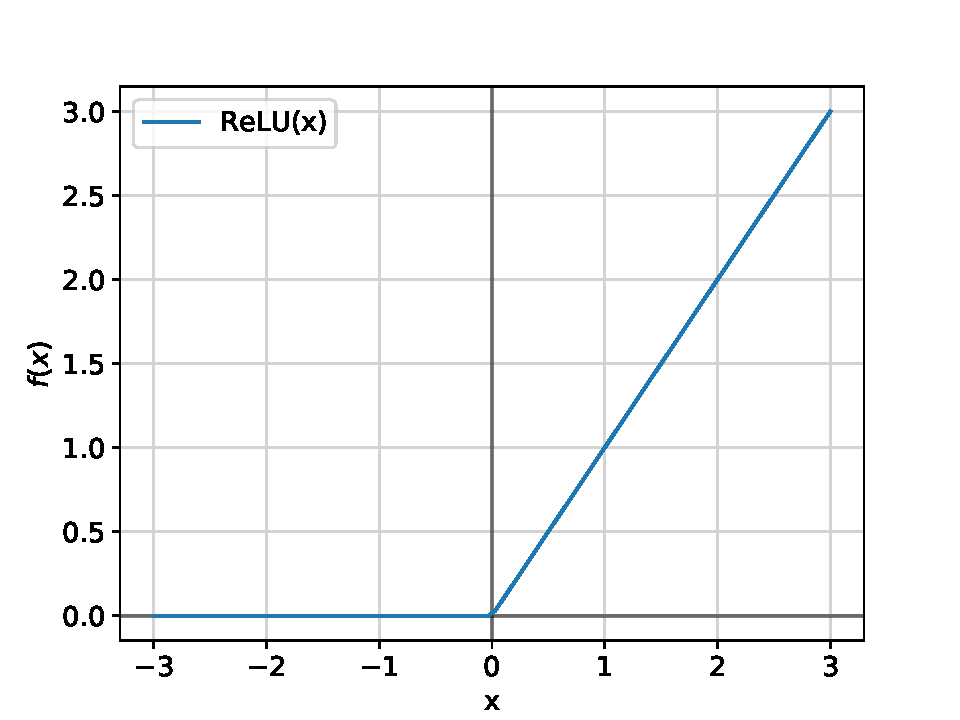
\includegraphics[width=7cm]{graphics/ReLU(x)}} 
	\subfloat[Leaky-ReLU: $f(\alpha, x) = \alpha x$ für $x<0$]{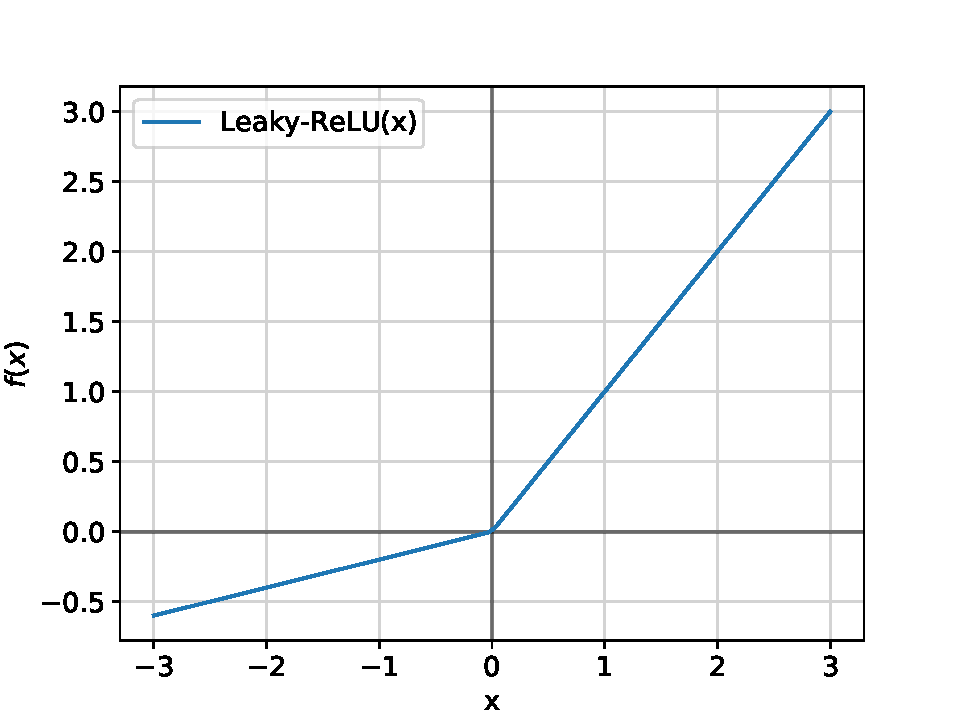
\includegraphics[width=7cm]{graphics/Leaky-ReLU(x)}} \\
	\subfloat[ELU: $f(\alpha, x) = \alpha(e^x - 1)$ für $x < 0$]{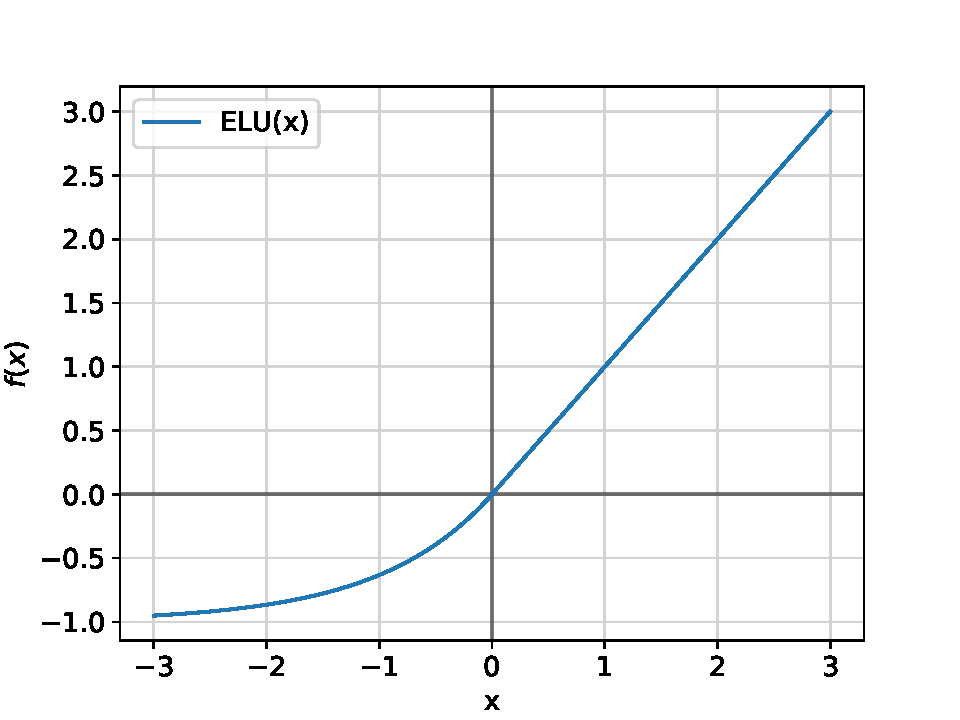
\includegraphics[width=7cm]{graphics/ELU(x)}}
	\subfloat[Sigmoid: $f(x) = \frac{e^x}{e^x + 1}$]{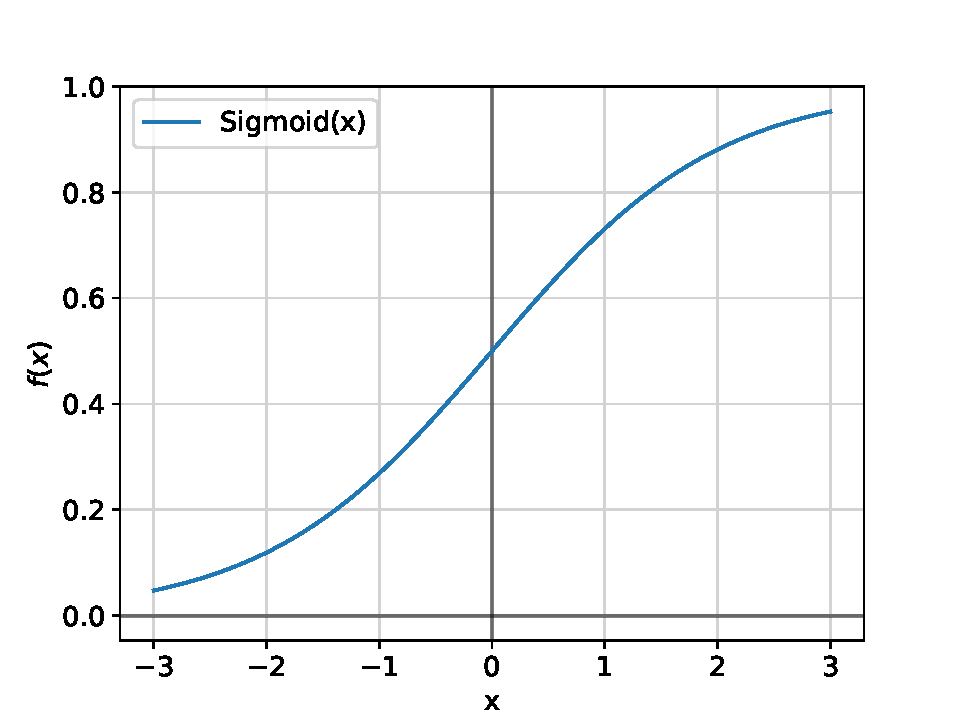
\includegraphics[width=7cm]{graphics/Sigmoid(x)}} \\
	\subfloat[tanh : $f(x) = tanh(x)$]{\includegraphics[width=7cm]{graphics/tanh(x)}}
	\subfloat[Exp: $f(x) = e^x$]{\includegraphics[width=7cm]{graphics/Exp(x)}} \\  
	\caption{Activation-Funkctions, die verwendet wurden}
	\label{11,27,28}
\end{figure}
\begin{table}
	\centering
	\begin{tabular}{|l|l|l|}
		\hline
		Hyperparameter & Pool & Best Config \\
		\hline
		Anzahl Layer & $\left\lbrace 1, 2, 3, 4 \right\rbrace$ & 4 \\
		Anzahl Units & $\left\lbrace 32, 64, 128, 256\right\rbrace$ & 128 \\
		Loss-Funktion & MAE, MSE, Huber & MAE \\
		Optimizer & Adam, RMSprop, SGD  & Adam\\
		Aktivierungsfunktion & ReLU, Leaky-ReLU, Sigmoid & Leaky-ReLU \\
		Learning-rate & $\left\lbrace 10^{-2}, 5 \cdot 10^{-3}, 10^{-3}, 10^{-4} \right\rbrace $ & $5 \cdot 10^{-3}$\\
		Batch-Größe & $\left\lbrace 64, 128, 512, 768, 2048 \right\rbrace $ & 128\\
		Label-Normalisierung & $\left\lbrace \text{keine}, [-1,1]\right\rbrace $ & $[-1,1]$\\
		\hline
		Max. Epochen & \multicolumn{2}{c|}{200}\\
		Anzahl Trainingspunkte & \multicolumn{2}{c|}{60000} \\
		\hline
	\end{tabular}
	\caption{Parameter der Random-Search für $\frac{d\sigma}{d\theta}$ mit Ergebnis}
\end{table}
\begin{table}
	\centering
	\begin{tabular}{|l|l|l|}
		\hline
		Hyperparameter & Pool & Best Config \\
		\hline
		(Units, Nr. of Layers) &$\left\lbrace (256,5), (512,3), (64,7), (1024, 2), (128, 6) \right\rbrace $ & $(256, 5)$ \\
		Loss-Funktion & MAE, MSE, Huber & MAE \\
		Optimizer & Adam, RMSprop  & Adam\\
		Aktivierungsfunktion & ReLU, Leaky-ReLU, Sigmoid, ELU, tanh & Leaky-ReLU \\
		Learning-rate & $\left\lbrace 10^{-2}, 5 \cdot 10^{-3}, 10^{-3}, 10^{-4} \right\rbrace $ & $10^{-2}$\\
		Batch-Größe & $\left\lbrace 256, 128, 512, 768, 1024 \right\rbrace $ & 256\\
		Basis 10 & True, False  & True \\
		Label-Normalisierung & $\left\lbrace \text{keine}, [-1,1]\right\rbrace $ & keine\\
		Feature-Normal. & True, False & True \\
		\hline
		Skalierung & \multicolumn{2}{c|}{True} \\
		Logarithmus & \multicolumn{2}{c|}{True} \\ 
		Max. Epochen & \multicolumn{2}{c|}{100}\\
		Trainingspunkte & \multicolumn{2}{c|}{4.000.000} \\
		\hline
	\end{tabular}
	\caption{Hyperparameter Pools eines erfolgreichen Random-Search mit bester Konfiguration für den dreidimensionalen differentiellen Wirkungsquerschnitt des Diphoton Prozesses}
\end{table}
\begin{table}
	\centering
	\begin{tabular}{|l|l|l|}
		\hline
		Hyperparameter & Pool & Best Config \\
		\hline
		Anzahl Layer & $\left\lbrace 1,2,3,4\right\rbrace$ & 2 \\
		Units &$\left\lbrace 32, 64, 128, 256\right\rbrace$ & 256 \\
		Loss-Funktion & MAE, MSE & MAE \\
		Optimizer & Adam, RMSprop, SGD  & Adam\\
		Aktivierungsfunktion & ReLU, Leaky-ReLU, Sigmoid & Leaky-ReLU \\
		Learning-rate & $\left\lbrace 10^{-2}, 5 \cdot 10^{-3}, 10^{-3}, 10^{-4} \right\rbrace $ & $5 \cdot 10^{-3}$\\
		Batch-Größe & $\left\lbrace 256, 128, 512, 768, 1024 \right\rbrace $ & 512\\
		Label-Normalisierung & $\left\lbrace \text{keine}, [-1,1]\right\rbrace $ & keine\\
		Feature-Normal. & True, False & True \\
		\hline
		Skalierung & \multicolumn{2}{c|}{False} \\
		Logarithmus & \multicolumn{2}{c|}{False} \\ 
		Max. Epochen & \multicolumn{2}{c|}{100}\\
		Trainingspunkte & \multicolumn{2}{c|}{1.000.000} \\
		\hline
	\end{tabular}
	\caption{Hyperparameter Pools eines Random-Search mit bester Konfiguration für ein Reweighting des differentiellen Wirkungsquerschnitt des Diphoton Prozesses}
\end{table}
\begin{table}
	\centering
	\begin{tabular}{|l|l|l|}
		\hline
		Hyperparameter & Pool & Best Config \\
		\hline
		Anzahl entfernte Layer & $\left\lbrace  1, 2 \right\rbrace $ & 1 \\
		Anzahl hinzugefügte Layer & $\left\lbrace  0, 1, 2 \right\rbrace $ & 1 \\
		Units(hinzugefügte Layer) &$\left\lbrace 64, 128, 512\right\rbrace$ & 128\\
		Aktivierungsfunktion & ReLU, Leaky-ReLU, Sigmoid & ReLU \\
		Learning-Rate & $\left\lbrace 10^{-2}, 5 \cdot 10^{-3}, 10^{-3}, 10^{-4} \right\rbrace $ & $5 \cdot 10^{-3}$\\
		Batch-Größe & $\left\lbrace 128, 512, 768, 2048, 8196 \right\rbrace $ & 768\\
		Fine-Tuning & True, False & True \\
		\hline
		Learning-Rate
		Loss-Funktion & \multicolumn{2}{c|}{MAE} \\
		Optimizer & \multicolumn{2}{c|}{Adam} \\
		Max. Epochen & \multicolumn{2}{c|}{100}\\
		Trainingspunkte & \multicolumn{2}{c|}{1.000.000} \\
		\hline
	\end{tabular}
	\caption{Hyperparameter Pools eines Random-Search mit bester Konfiguration für Transfer-Learning zwischen Wirkungsquerschnitten verschiedener PDF-Sets}
\end{table}
% TODO gar nicht wahr, die dinger sind abh. von batch size
\begin{table}
	\centering
	\begin{tabular}{|l|l|}
		\hline
		Callback & Config \\
		\hline
		\multirow{3}{*}{LearningRateScheduler} & nach einem Offset von 10 Epochen, wird die \\
		& Learning-Rate nach jeder Epoche um $5\%$ reduziert, \\
		& bis diese auf $5 \cdot 10^{-8}$ abgefallen ist. \\
		\hline
		\multirow{2}{*}{ReduceLROnPlateau}& Fällt der Loss nach einer Epoche nicht um mindestens\\
		& $2 \cdot 10^{-6}$, wird die Learning-Rate um $50\%$ reduziert.\\
		\hline
		\multirow{3}{*}{EarlyStopping}& Fällt der Loss in drei aufeinanderfolgenden \\
		& Epochen nicht um $2 \cdot 10^{-7}$ ab, \\
		& wird der Trainingsvorgang gestoppt.\\
		\hline
	\end{tabular}
	\label{callbacks}
\end{table}
\section{Abkürzungen}
\begin{table}[htp]
	\centering
	\begin{tabular}{ll}
		ML $\hspace{3cm}$& Machine-Learning \\
		TL & Transfer-Learning \\
		DNN & Deep-Neural-Network \\
		PDF & Partondichtefunktion \\
		MC & Monte-Carlo \\
		Features & Eingabewerte eines ML-Algorithmus \\
		Labels & wahrer Funktionswert der Features \\
		Units & Neuronen, Grundbaustein des DNN \\
		Nodes & Neuronen, Grundbaustein des DNN \\
		Layer & Schicht von Neuronen \\
		MSE & Mean-Squared-Error, mittlere quadratische Abweichung \\
		MAE & Mean-Absolute-Error, mittlere absolute Abweichung \\
		MAPE & Mean-Absolute-Percentage-Error\\
		MSLE & Mean-Squared-Logarithmic-Error \\
		Base 10& Daten werden mit Logarithmus zur Basis 10 transformiert \\
		FN & Feature-Normalization \\
		LN & Label-Normalization \\
		Log & Nur Scaling+Logarithmus \\
		No Log & Nur Scaling\\
		FT & Fine-Tuning \\
		TPM & Time per Million, Zeit die das DNN benötigt, um $10^6$ Phasenraumpunkte zu evaluieren \\
		&\\
	\end{tabular}
	\caption{Häufig genutzte Abkürzungen und Fachvokabular}
\end{table}

\section{Grafiken}
\section{Source-Code}

%--------------------------------------------------------------------
% Vorlage für eine Abschlussarbeit
% Darf ohne Einschränkungen weiterverwendet und abgeändert werden.
% mehr zur Verwedung in der README.md
% ⓒ (CC0) 2016, 2018 Henning Iseke <h_i_@online.de>
%--------------------------------------------------------------------

\printbibliography
\cleardoublepage
\pagestyle{empty}
\section*{Danksagung} % TODO: anpassen
Danke an Christial Wiel.
\cleardoublepage
%TODO: anpassen
\section*{Erklärung}
Hiermit erkläre ich, dass ich die vorliegende Arbeit im Rahmen der Betreuung am
\institut{} ohne unzulässige Hilfe Dritter verfasst habe und alle verwendeten
Quellen als solche gekennzeichnet habe.

% Zur Beschriftung
\vspace{5\baselineskip}
\noindent
\rule[0.5ex]{20em}{0.5pt}\rule[0.5ex]{10em}{0.5pt}\\
Ort, Datum\hspace{8em}Unterschrift 

%
%--------------------------------------------------------------------
% Vorlage für eine Abschlussarbeit
% Darf ohne Einschränkungen weiterverwendet und abgeändert werden.
% mehr zur Verwedung in der README.md
% ⓒ (CC0) 2016, 2018 Henning Iseke <h_i_@online.de>
%--------------------------------------------------------------------

\printbibliography
\cleardoublepage
\pagestyle{empty}
\section*{Acknowledgements} % TODO: anpassen, britsh english
<Thank you>
\cleardoublepage
\begin{german}
\section*{Erklärung} 
%TODO: anpassen
Hiermit erkläre ich, dass ich die vorliegende Arbeit im Rahmen der Betreuung am
\institut{} ohne unzulässige Hilfe Dritter verfasst habe und alle verwendeten
Quellen als solche gekennzeichnet habe.

% Zur Beschriftung
\vspace{5\baselineskip}
\noindent
\rule[0.5ex]{20em}{0.5pt}\rule[0.5ex]{10em}{0.5pt}\\
Ort, Datum\hspace{8em}Unterschrift
\end{german}

\end{document}
\begin{table}
\centering
\begin{tabular}{lll}
	Integrand & \multicolumn{2}{l}{$\quad \sigma_{tot}$[pb]} \\
	\hline
	analytic & & \\
	prediction & & \\
\end{tabular}
\end{table}

\begin{itemize}
\setlength\itemsep{0.1cm}
\setlength{\parskip}{0.1cm}
\item Anzahl der Layer l: $\left\lbrace2, 3\right\rbrace$  
\item Anzahl der Knoten pro Layer: $\left\lbrace64, 128 \right\rbrace $
\item Kostenfunktion: $\left\lbrace \text{MeanSquaredError}, \text{MeanAbsoluteError} \right\rbrace$
\item Optimizer: $\left\lbrace \text{Adam}, \text{SGD} \right\rbrace$
\item Learning-rate $\left\lbrace 10^{-3}, 10^{-4}, 10^{-5} \right\rbrace$
\item batch-size $\left\lbrace 32, 64 \right\rbrace$
\item Epochen: $\left[1,50\right]$
\end{itemize}

Um die Hyperparameter festzulegen, nutzen wir ein Grid-Search und überprüfen nach jedem Trainingsdurchgang, ob sich das Ergebnis des Algorithmus verbessert hat. Wir variieren dabei die folgenden Werte in den Bereichen:

Wir beurteilen am Ende jedes Durchgangs das Modell nach den folgenden Kriterien: Genauigkeit, Trainingszeit, Performance. Genauigkeit und Trainingszeit sind dabei selbsterklärend, Performance meint die Rechenaufwändigkeit eines fertigen Modells bei der Anwendung auf Testdaten. Wir können so ein systematisches Modell zur Erstellung und Bewertung von neuronalen Netzen erhalten, das wir auf zukünftige Probleme übertragen können.

Für die Hyperparameter wurden mittlereweile zwar Algorithmen entwickelt, die effizienter sein sollen als ein Random Search, in dieser Arbeit konnte jedoch keine Verbesserung festgestellt werden. Konkret ausprobiert wurden ein "Bayesian Search" und der "Hyperband-Tuner", wobei die Implementierung mit Keras-Tuner vollzogen wurde. Bayesian Search benutzt eine Objecitv-Funktion, die aus den bereits getesteten Hyperparametern eine Vorhersage für vielversprechende neue Hyperparameter-Kombinationen abgibt. Hyperband trainiert eine große Zahl an Modellen für wenige Epochen und sucht aus diesen die besten Kandidaten zum Weitertrainieren aus. Dies wird stufenweise durchgeführt, bis man in der Theorie mit einer Hand voll gut funktionierender Hyperparameter zurückbleibt.

%TODO Faktor 1/2 bei partonischem WQ
%TODO 32,33 neumachen